% Phase 1 report, M.Tech. Project, Suhas H, roll number 25M0328, CSRE, IIT Bombay.
% Main file. Each chapter lives in its own file and is pulled in with \include.
% Compile from the report/ folder of the repository, so that ../figures/ resolves.

\documentclass[12pt,a4paper]{report}

% ===========================================================================
% Page and type
% ===========================================================================
\usepackage[a4paper,left=1.25in,right=1in,top=1in,bottom=1in,headheight=15pt]{geometry}
\usepackage[T1]{fontenc}
\usepackage{palatino}            % URW Palladio for text, Computer Modern for maths
\usepackage{microtype}
\usepackage{setspace}
\setstretch{1.25}
\usepackage{parskip}             % blank line between paragraphs, no indent

\usepackage{amsmath,amssymb}
\usepackage{graphicx}
\graphicspath{{../figures/}}
\usepackage{booktabs}
\usepackage{array}
\usepackage{tabularx}
\usepackage{enumitem}
\setlist{itemsep=2pt,topsep=4pt}
\usepackage[font=small,labelfont=bf]{caption}
\usepackage{float}

% Chapter heading in two lines, left aligned: "Chapter 1", then the title
\usepackage{titlesec}
\titleformat{\chapter}[display]
  {\normalfont\bfseries}{\Large\chaptertitlename\ \thechapter}{18pt}{\huge}
\titlespacing*{\chapter}{0pt}{0pt}{28pt}
\titleformat{\section}{\normalfont\Large\bfseries}{\thesection}{1em}{}
\titleformat{\subsection}{\normalfont\large\bfseries}{\thesubsection}{1em}{}

% Running header: "CHAPTER N. TITLE" on the left, page number on the right
\usepackage{fancyhdr}
\pagestyle{fancy}
\fancyhf{}
\fancyhead[L]{\footnotesize\leftmark}
\fancyhead[R]{\footnotesize\thepage}
\renewcommand{\headrulewidth}{0.4pt}
\renewcommand{\chaptermark}[1]{\markboth{\MakeUppercase{\chaptername\ \thechapter.\ #1}}{}}
\fancypagestyle{plain}{\fancyhf{}\fancyfoot[C]{\thepage}\renewcommand{\headrulewidth}{0pt}}

\usepackage{xcolor}
\usepackage[colorlinks=true,linkcolor=blue!50!black,
            citecolor=blue!50!black,urlcolor=blue!50!black]{hyperref}

\setlength{\emergencystretch}{3em}
% Long file names in the file map may break after an underscore or a hyphen
\expandafter\def\expandafter\UrlBreaks\expandafter{\UrlBreaks\do\_\do\-}
\renewcommand{\bibname}{References}

% Subscripts in chemical formulae, in the text typeface: SO\sub{2}
\newcommand{\sub}[1]{\textsubscript{#1}}

\begin{document}

% Title page, laid out after page one of the department's M.Tech. sample.
\begin{titlepage}
  \centering
  \setstretch{1.0}
  \vspace*{0cm}
  {\LARGE\bfseries Venus Photochemistry\par}
  \vspace{1.0cm}
  {\normalsize Phase 1 Report submitted in partial fulfilment of the requirements\\
   for the award of the degree of\par}
  \vspace{1.0cm}
  {\Large\bfseries Master of Technology\par}
  \vspace{0.5cm}
  {\normalsize by\par}
  \vspace{0.5cm}
  {\Large\bfseries Suhas H\par}
  \vspace{0.2cm}
  {\normalsize Roll Number: 25M0328\par}
  \vspace{0.6cm}
  {\normalsize Under the Supervision of\par}
  \vspace{0.3cm}
  {\Large\bfseries Prof. Deepak Singh\par}
  \vspace{0.6cm}
  
\includegraphics[width=3.6cm]{iitb-logo}\par
  \vspace{0.6cm}
  {\large Geoinformatics and Natural Resources Engineering\par}
  \vspace{0.3cm}
  {\large Centre of Studies in Resources Engineering\par}
  \vspace{0.4cm}
  {\Large\bfseries INDIAN INSTITUTE OF TECHNOLOGY BOMBAY\par}
  \vspace{0.4cm}
  {\large\bfseries Mumbai -- 400076, India\par}
  \vspace{0.4cm}
  {\large October 2026\par}
\end{titlepage}


% Front matter, numbered in roman numerals
\pagestyle{plain}
\pagenumbering{roman}
% Acknowledgment. A draft in the style of the author's seminar report, for him to edit.
\chapter*{Acknowledgment}
\phantomsection
\addcontentsline{toc}{chapter}{Acknowledgment}

I extend my sincere gratitude to my supervisor, Prof.\ Deepak Singh, for his guidance
throughout Phase~1 of this project, for the direction that shaped its questions, and for
his constructive feedback on this report.

I thank L.\ Dai, W.\ Shao and Z.\ Sheng, the authors of VULCAN-Venus, for making
their model openly available, and T.\ Trabelsi and J.\ S.\ Francisco for providing the computed cross sections used in Experiment~11.

\vspace{1cm}
\begin{flushright}
Suhas H\\
Roll Number: 25M0328\\
CSRE, IIT Bombay
\end{flushright}

% Abstract. Every number here comes from verify/registry.json.
\chapter*{Abstract}
\phantomsection
\addcontentsline{toc}{chapter}{Abstract}
\begingroup\setstretch{1.15}

Something in the clouds of Venus absorbs near-ultraviolet sunlight and is responsible for
about half of the solar heating at the cloud top, yet nearly a century after its markings
were first photographed, the substance is still unknown. This project asks not which
molecule has the right spectrum but whether any proposed carrier can be present in
the right amount, at the right altitude and with the right spectral shape, all at once,
inside a model that is free to move it around.

The work uses VULCAN-Venus, a one-dimensional model of the photochemistry of the Venus
atmosphere. Phase~1 found that the model's absorber term was present but switched off,
switched it on under a single amplitude, and ran fourteen experiments on the model and
on published laboratory data. Every number is
recomputed from the saved model output by one script into a registry of 10830 values,
and a second script checks every printed number precise enough to test against it.

The absorber's effect on the radiation is proportional to its amount and is concentrated
in one band of altitude, 69 to 93~km, which holds 91.370\% of the response. Where an
absorber sits matters more than its spectrum: moved up, the same absorber changes the
radiation 7.34 times more than moved down, against a factor of 4.95 between the
spectra tested at a fixed height. When the model's own chemistry is allowed to place
ClS\sub{2}, the gas closest to the needed amount, its centre falls 51.521~km lower and
it becomes radiatively the same as no absorber, to 0.001487\%. A screen of all 23
species the model can represent finds none that passes amount, placement and spectrum
together. From published data, the proposed iron and sulfur minerals cannot absorb enough at 375~nm even as pure solids, and a
published rejection of ferric chloride, based on a measurement in water, does not hold
if it absorbs in the droplets as it does in hydrochloric acid, where the amount needed
falls from 71.0\% of the droplet mass to between 2.82\% and 17.05\%. Changes in
abundance smaller than 2.5278\% are shown to be numerical, not physical, and are
reported only as upper bounds.

Phase~2 proposes to test these verdicts under the much stronger vertical mixing now
estimated for the Venus clouds, to ask whether upwelling can carry a candidate into the
response band, and to place ferric chloride by the same altitude test.

\textbf{Keywords:} Venus, unknown ultraviolet absorber, photochemistry, VULCAN,
radiative transfer, ferric chloride, reproducibility
\par\endgroup

{\setstretch{1.1}
\tableofcontents
\cleardoublepage\phantomsection\addcontentsline{toc}{chapter}{List of Figures}
\listoffigures
\cleardoublepage\phantomsection\addcontentsline{toc}{chapter}{List of Tables}
\listoftables
}
% List of terms. Each entry restates the definition given in the chapter named.
\chapter*{List of Terms}
\phantomsection
\addcontentsline{toc}{chapter}{List of Terms}

{\setstretch{1.1}
\begin{description}[leftmargin=0pt, itemsep=3pt]
  \item[Absorber grid.] 300 to 698~nm, the wavelengths over which the absorber term acts
    (Chapter~4).
  \item[Absorption efficiency, $Q_{\mathrm{abs}}$.] The fraction of the light falling on a
    particle's cross-sectional area that the particle absorbs; the absorber's spectrum is a
    table of it (Chapter~3).
  \item[Actinic flux.] The number of photons per square centimetre per second per
    nanometre reaching a point from all directions; it sets every photolysis rate
    (Chapter~3).
  \item[Amplitude, $A_{\mathrm{UUV}}$.] The single number that scales the absorber term:
    0 for the control, 1 for the supplied absorber, and 0.5 and 2 in Experiment~3
    (Chapters~3 and~5).
  \item[Baseline and reference.] The reference is the output supplied with the model,
    kept untouched; the baseline is the same model run afresh on the project computer
    (Chapter~3).
  \item[Bounded mean.] A mean over a field that leaves out the elements where both values
    are zero (Chapter~4).
  \item[Cloud top.] The height at which the cloud's optical depth, counted downward from
    space, reaches one (Chapter~1).
  \item[Column and column centre.] A quantity per cubic centimetre added over altitude
    with each layer thickness in centimetres, giving a quantity per square centimetre; the
    column centre, or centroid, is the mean altitude weighted by that quantity (Chapters~3
    and~4).
  \item[Control and treatment.] Two runs that differ only in the absorber: switched off
    in the control, switched on in the treatment (Chapter~3).
  \item[Cross section.] The effective area one molecule presents to light, in square
    centimetres (Chapter~3).
  \item[Decadic and Napierian.] Absorbance measured with base-10 and with natural
    logarithms; the two differ by a factor of $\ln 10$ (Chapters~2 and~6).
  \item[Eddy diffusion coefficient, $K_{zz}$.] The strength of vertical mixing in the
    model (Chapters~2 and~3).
  \item[Empirical absorber.] The absorber supplied with the model, a spectrum and a
    height profile fitted to the observed brightness of Venus (Chapters~1 and~3).
  \item[Enhancement band.] 320 to 400~nm, the near-ultraviolet feature the absorber has
    to supply (Chapter~4).
  \item[Field change, $\Delta F$.] The size of the change in the whole actinic flux
    field, as a percentage of the size of the reference field (Chapter~4).
  \item[Isomers.] Molecules made of the same atoms arranged differently, such as ClSSCl
    and SSCl\sub{2} (Chapters~2 and~6).
  \item[Loading.] The mass of a candidate needed per litre of droplet to meet the
    absorption requirement (Chapter~6).
  \item[Mass absorption coefficient, $\varepsilon$.] How strongly a material absorbs per
    gram, in square centimetres per gram; dividing the required absorption by it gives
    the loading (Chapter~6).
  \item[Mixing ratio.] The number density of a species divided by that of the air,
    quoted in parts per million (ppmv) or per billion (ppb) (Chapters~2 and~3).
  \item[Mode~1 droplets.] Cloud droplets smaller than one micrometre across, in which the
    absorber is thought to sit (Chapter~1).
  \item[Optical depth.] A measure of how much light a layer removes; light crossing an
    optical depth of one keeps a fraction $e^{-1}$ of its intensity (Chapters~1 and~3).
  \item[Photolysis.] The breaking of a molecule by a photon. Its rate coefficient $J$ is
    the probability per second that one molecule is broken; the rate $J n$ also depends
    on how much of the molecule is present (Chapters~3 and~4).
  \item[Radiation floor.] 0.0017\%: how far the radiation fields of two runs that should
    agree differ, as a share of the change Experiment~9 makes, not of the whole field
    (Chapters~4 and~6).
  \item[Reflectivity, $I/F$.] The observed radiance divided by $\pi F_\odot$, where
    $F_\odot$ is the solar flux arriving at Venus (Chapter~1).
  \item[Registry and key.] The file \texttt{verify/registry.json} that holds every
    number in this report, and the dotted name of each value in it (Chapter~8).
  \item[Relative change.] A difference divided by the larger of the two values, not by
    the control (Convention~1, Chapter~4).
  \item[Reproducibility floor, or chemistry floor.] 2.5278\%: in-band changes in abundance
    smaller than this are numerical, not physical, and are reported only as upper bounds
    (Chapter~4).
  \item[Requirement constant, $\tau_{\mathrm{req}}$.] The empirical absorber's optical
    depth through the whole atmosphere at 320~nm, the amount of absorption any candidate
    must supply (Chapter~3).
  \item[Response band and centroid.] The narrowest range of altitude, 69 to 93~km, that
    holds at least 90 per cent of the radiative response, and the weighted mean
    altitude of that response (Chapter~4).
  \item[Screening window.] 300 to 620~nm, the range searched for each candidate's
    strongest absorption (Chapter~4).
  \item[Shortfall factor.] How many times too little of a species the model holds to
    supply the required optical depth (Chapter~6).
  \item[Single scattering albedo.] The fraction of light meeting a particle that is
    scattered rather than absorbed (Chapter~2).
  \item[Spectral correlation.] How closely a candidate's spectrum follows the empirical
    absorber's, as a correlation coefficient between $-1$ and 1 (Chapter~6).
  \item[Steady state.] The state in which production, destruction and transport of every
    species balance, tested by \texttt{longdy} and \texttt{longdydt} (Chapters~1 and~3).
  \item[Super-rotation.] The flow of the atmosphere at the cloud top round the planet far
    faster than the planet itself turns (Chapter~1).
  \item[Weight per cent, wt\%.] The share of a mixture's mass that one component makes
    up (Chapter~2).
\end{description}
\par}


% Main text, numbered from 1
\cleardoublepage
\pagestyle{fancy}
\pagenumbering{arabic}
% Chapter 1. Introduction.
% Every number in this chapter comes from verify/registry.json, from
% figures/literature_values.json, or from the paper cited next to it.

\chapter{Introduction}
\label{ch:intro}

This report describes Phase 1 of an M.Tech.\ project on the atmosphere of Venus. It
starts from the first reading of the literature and ends with the proposal for Phase 2.
The subject is a single long-standing problem: something in the clouds of Venus absorbs
near-ultraviolet sunlight, and nobody knows what it is. This chapter explains what is
known about that problem, what has been tried, and how this project approaches it
differently.

\section{Venus and its clouds}
\label{sec:venus}

Venus has a thick atmosphere. The pressure at the surface reaches 92 bar and the surface
temperature is about 750~K~\cite{dai2025review}. The planet is completely covered by a
dense cloud deck that lies between 47 and about 70~km above the surface and is more than
20~km thick~\cite{dai2025review}. The clouds are made of small droplets of concentrated
sulfuric acid, H\sub{2}SO\sub{4}~\cite{dai2025review}.

Measurements made by a descent probe divide the cloud deck into three layers by the mass
of cloud material they hold: the lower cloud, from about 48 to 50~km; the middle cloud,
from about 50 to 56~km; and the upper cloud, from about 56 to 70~km~\cite{dai2025review}.
The droplets are also grouped by size into \emph{modes}. Mode~1 droplets are smaller than
one micrometre across and are the most numerous throughout the cloud deck; mode~2
droplets are about two micrometres across~\cite{dai2025review}. Mode~1 matters for this
report because the unknown absorber is now thought to be mixed into mode~1
droplets~\cite{dai2025review,perezhoyos2018}.

The \emph{cloud top} is defined as the height at which the optical depth of the cloud,
counted downward from space, reaches one~\cite{dai2025review}. Optical depth is a
measure of how much light a layer removes: light that crosses an optical depth of one
keeps a fraction $e^{-1}$, about a third, of its original intensity. Depending on the
wavelength used and the place observed, the cloud top lies between 65 and
72~km~\cite{dai2025review}.

The solid planet turns very slowly. One rotation relative to the stars takes 243 Earth
days, and one solar day, from noon to noon, takes 117 Earth days~\cite{bertaux2016}. The
atmosphere at the cloud top moves far faster. It travels westward round the planet in
about four days, with a wind speed of about 100 metres per
second~\cite{bertaux2016}; in the cloud layer as a whole the circuit takes 4 to 6
days~\cite{limaye2018}. This fast circulation is called \emph{super-rotation}. It was
first revealed by ultraviolet observations of the cloud markings (Ross, 1928, and Boyer
and Camichel, 1961, as cited in~\cite{perezhoyos2018}), which is the first sign that the
ultraviolet appearance of Venus and its atmospheric motion are linked.

Figure~\ref{fig:F1} summarises this structure. It also shows two things that come from
the present project and are explained later: the grey band, which marks the altitudes
where the model's radiation responds to the absorber (Chapter~5), and the altitudes where
the model's own chemistry places a set of candidate molecules (Chapter~6).

\begin{figure}[htbp]
  \centering
  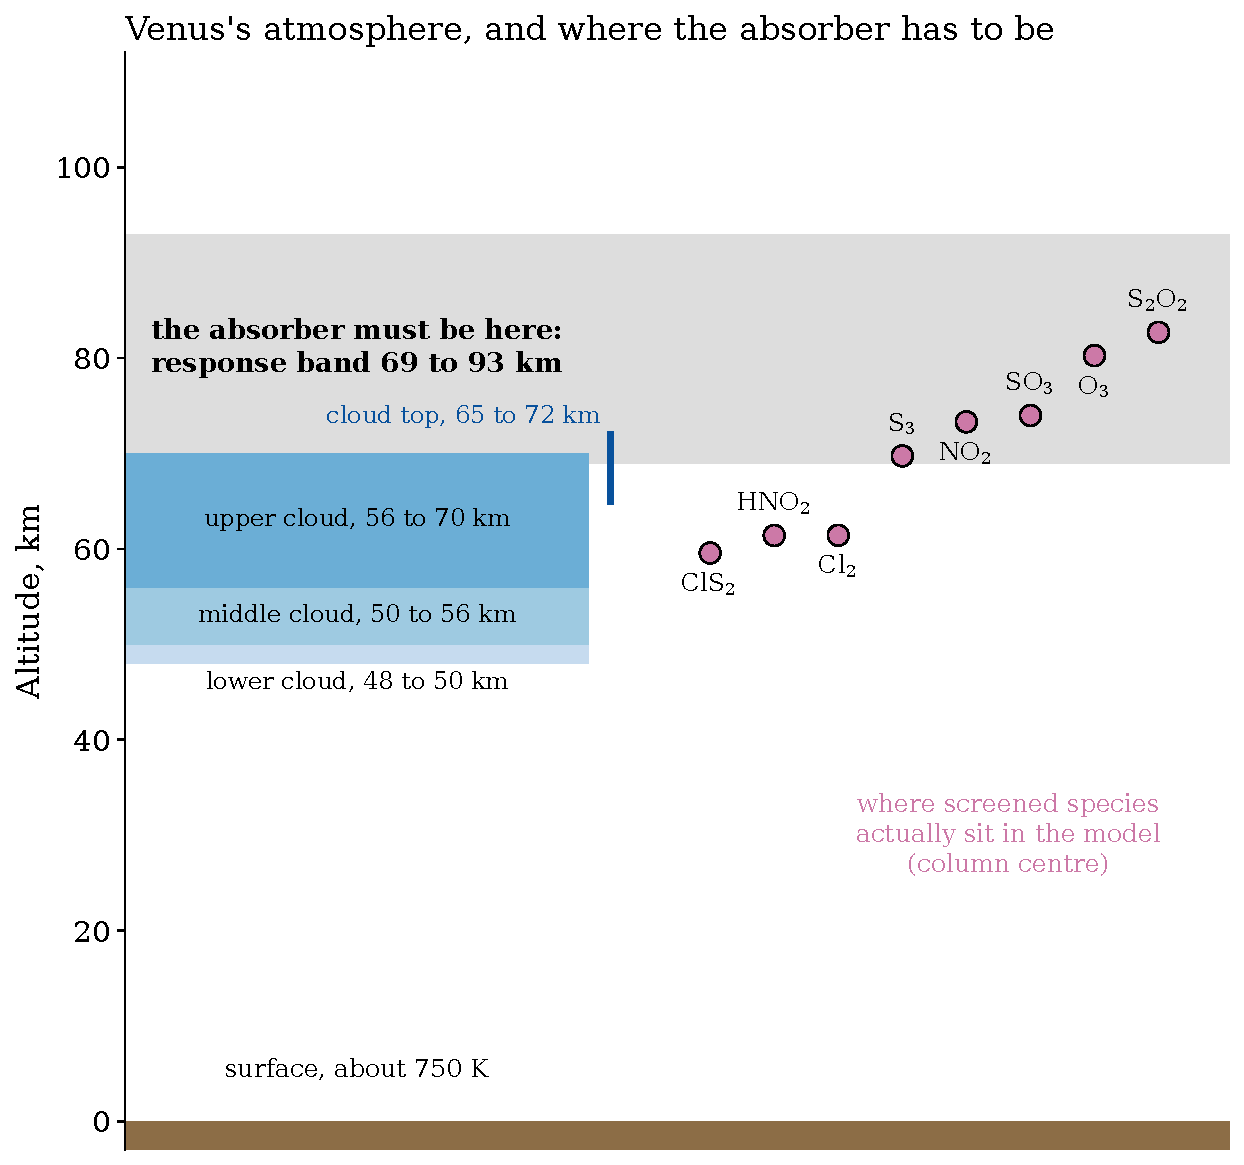
\includegraphics[width=0.68\textwidth]{F01_CTX_venus-atmosphere_ch1_s3.pdf}
  \caption[The Venus atmosphere, and where the absorber has to be]{The Venus atmosphere, and where the absorber has to be. Left: the three cloud
    layers and the range of cloud top heights, from~\cite{dai2025review}; the surface
    temperature, from the same source. Grey band: the response band, 69 to 93~km,
    found in Experiment~6 (Chapter~5). Purple circles: the column centre of eight
    candidate molecules as placed by the model's own chemistry (Experiment~12).
    Sources: \texttt{figures/literature\_values.json}; registry keys
    \texttt{e6.interval.90.lo}, \texttt{e6.interval.90.hi} and
    \texttt{e12.<species>.centroid}.}
  \label{fig:F1}
\end{figure}

\section{The unknown ultraviolet absorber}
\label{sec:absorber}

In visible light Venus is very bright: its clouds scatter about 80 per cent of the
incoming sunlight back to space~\cite{dai2025review}. Towards the ultraviolet the planet
becomes darker, and the darkening has two parts. Below 320~nm the shape of the absorption
matches sulfur dioxide, SO\sub{2}, which is therefore taken to be responsible for
it~\cite{dai2025review}. But SO\sub{2} absorbs only weakly at longer wavelengths, and its
effect is negligible beyond 320~nm~\cite{perezhoyos2018}. Between 320 and 400~nm there is
a second, strong absorption that no known species has been shown to
explain~\cite{dai2025review}. In the spectrum of the planet it appears as a broad band
reaching from the near ultraviolet into the blue~\cite{perezhoyos2018}. Because its
carrier is not known, it is called the \emph{unknown ultraviolet
absorber}~\cite{dai2025review}. In this report it is called simply \emph{the absorber}.

Figure~\ref{fig:F2} shows the problem directly. The upper panel is one reflectivity
spectrum of Venus, number 151, measured by the MESSENGER spacecraft during its second
Venus flyby on 5 June 2007~\cite{perezhoyos2018}. Reflectivity, written $I/F$, is the observed radiance divided
by $\pi F_\odot$, where $F_\odot$ is the solar flux arriving at Venus~\cite{perezhoyos2018}:
a perfectly white, evenly scattering surface lit from directly overhead would have
$I/F = 1$. The lower panel is the
absorption cross section of SO\sub{2} used in the model, which measures how strongly one
SO\sub{2} molecule absorbs at each wavelength. Venus is dark between 320 and 400~nm, which
is exactly where SO\sub{2} has almost stopped absorbing. From the same MESSENGER data,
P\'erez-Hoyos et al.\ found the absorption to be centred near 340~nm with a full width at
half maximum of about 140~nm~\cite{perezhoyos2018}.

\begin{figure}[htbp]
  \centering
  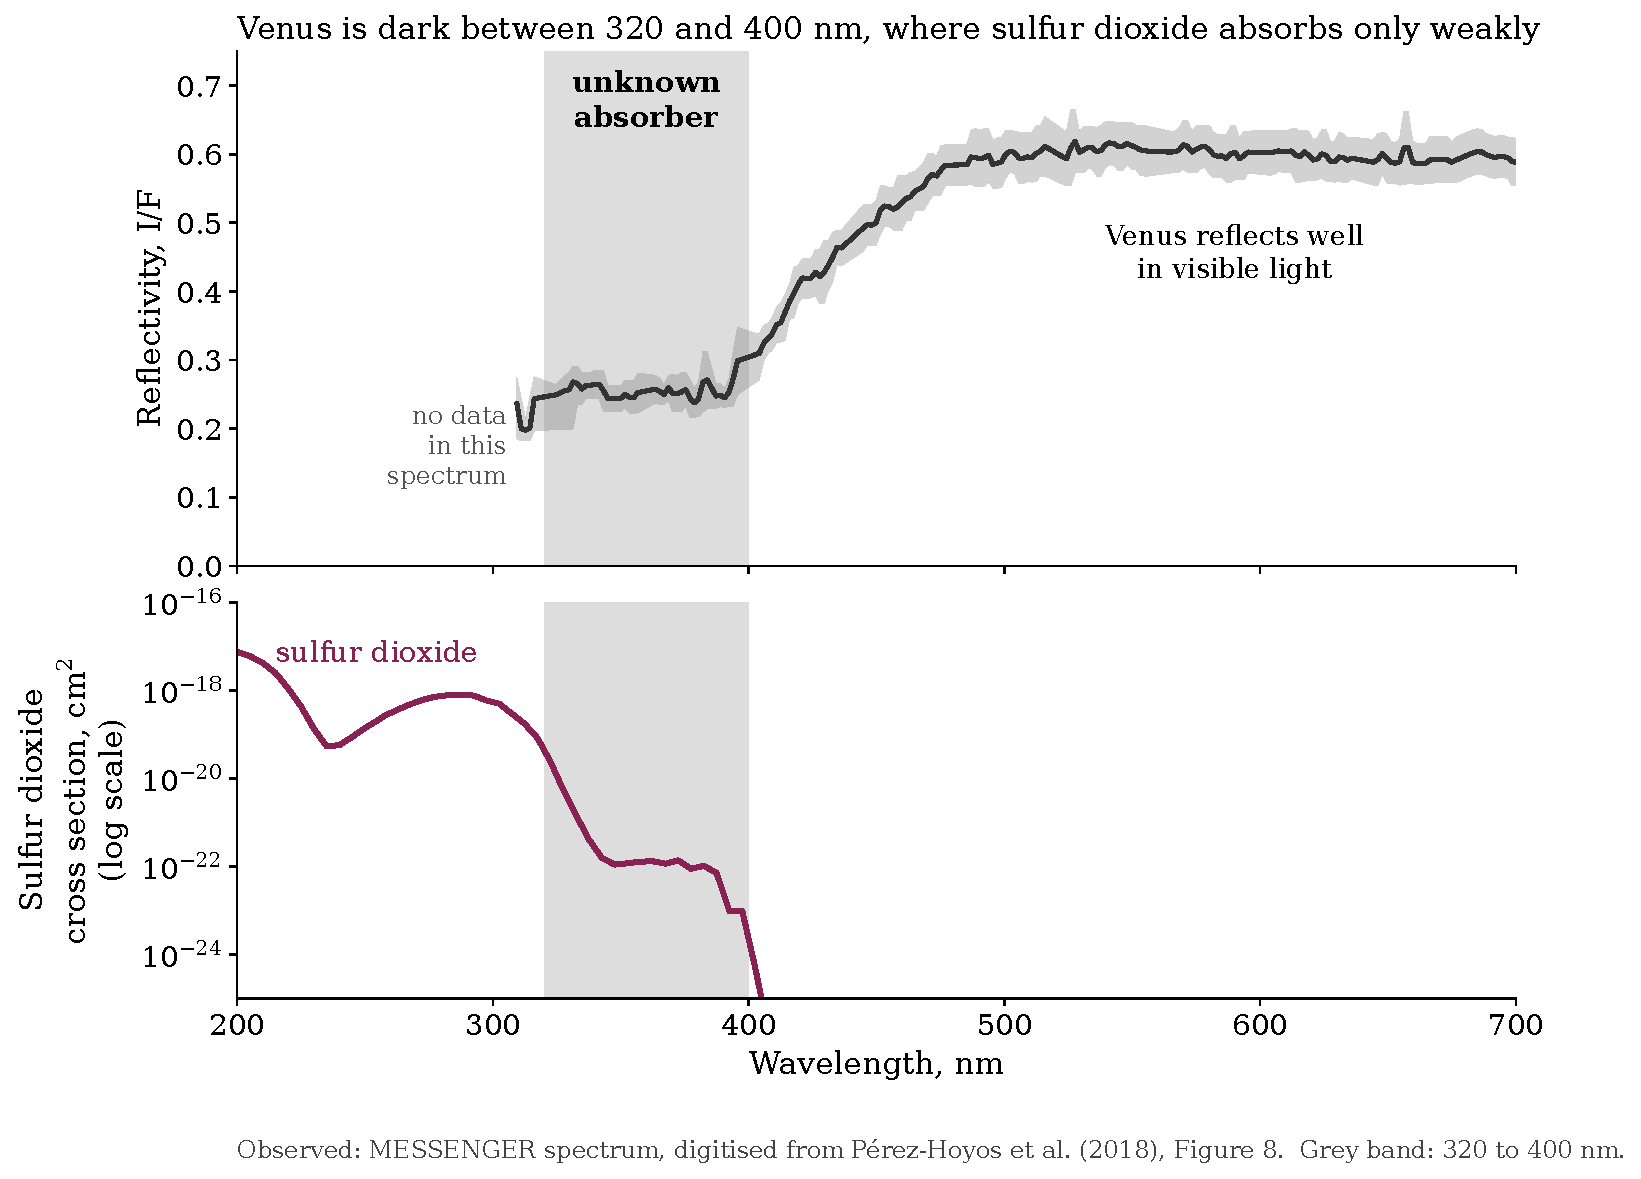
\includegraphics[width=0.74\textwidth]{F02_CTX_observed-uv-absorption_ch1_s2.pdf}
  \caption[Venus is dark between 320 and 400~nm, where sulfur dioxide absorbs only weakly]{Venus is dark between 320 and 400~nm, where sulfur dioxide absorbs only
    weakly. Top: observed reflectivity $I/F$ of MESSENGER spectrum 151, digitised from
    Figure~8 of P\'erez-Hoyos et al.~\cite{perezhoyos2018}; the shaded envelope is the
    drawn observation with its plotted error range, and the line its middle. Bottom: the SO\sub{2} absorption cross section used in
    the model, on a logarithmic scale. Sources:
    \texttt{figures/data/perez-hoyos-2018-fig8-IF.csv} (with its provenance file) and
    \texttt{thermo/photo\_cross/SO2/SO2\_cross.csv}.}
  \label{fig:F2}
\end{figure}

The absorber matters for three reasons.

\textbf{It heats the cloud top.} Observations and models agree that the absorber is
responsible for about half of the solar heating at the cloud top~\cite{dai2025review}.
Solar heating in the upper clouds has in turn been proposed as one of the engines of the
super-rotation, through the thermal tides it excites~\cite{perezhoyos2018}.

\textbf{It changes over time, and the circulation changes with it.} The brightness of
Venus at 365~nm varied strongly between 2006 and 2017, which implies that the amount of
absorber varied by a factor of two; the resulting change in solar heating has been
proposed to alter the strength of the Hadley circulation, the large overturning flow
between the equator and the poles (Lee et al.,
2019, as reviewed in~\cite{dai2025review}).

\textbf{Its pattern traces vertical motion.} The dark and bright markings seen in
ultraviolet images are not random. At low latitudes the clouds are dark because
convection brings the absorber up from below; at middle latitudes a cold layer with a
stable temperature profile suppresses vertical mixing and cuts off that supply, so the
clouds there are bright and uniform~\cite{titov2008}. In other words, where the absorber
appears depends on how the atmosphere moves it up and down. This observation is the
starting point of the present project.

What is known about \emph{where} the absorber sits is limited. Measurements of sunlight
made by descent probes found that ultraviolet absorption happens mainly in the upper
cloud, above about 57~km, and is negligible in the middle and lower clouds (Tomasko et
al., 1980, and Ekonomov et al., 1984, as reviewed in~\cite{dai2025review}). The supply of
absorber from below appears to be continuous at low latitudes~\cite{dai2025review}.
Nearly a century after the ultraviolet contrasts were first photographed from Earth, the
substance that causes them is still unknown~\cite{limaye2018}.

\section{The candidates proposed so far}
\label{sec:candidates}

Many substances have been put forward as the absorber. Table~\ref{tab:candidates} lists
the main ones, as summarised in a recent review~\cite{dai2025review} and in the
MESSENGER study~\cite{perezhoyos2018}. The table is a summary for orientation; Chapter~2
reviews the key papers one by one.

\begin{table}[htbp]
  \centering
  \caption[The main candidates for the unknown absorber, what supports each, and what counts against it]{The main candidates for the unknown absorber, what supports each, and what
    counts against it. Proposers are given as cited in the sources in the last column.}
  \label{tab:candidates}
  \footnotesize
  \setstretch{1.0}
  \begin{tabularx}{\textwidth}{>{\raggedright\arraybackslash}p{2.6cm}
                                >{\raggedright\arraybackslash}X
                                >{\raggedright\arraybackslash}X
                                >{\raggedright\arraybackslash}p{1.3cm}}
    \toprule
    Candidate & In its favour & Against it & Source \\
    \midrule
    Sulfur dioxide, SO\sub{2} &
      Matches the absorption below 320~nm. &
      Negligible beyond 320~nm, so it cannot supply the band between 320 and 400~nm. &
      \cite{perezhoyos2018,dai2025review} \\
    Polysulfur, S\sub{x} (Hapke and Nelson, 1975) &
      One of the first candidates considered for its spectral properties. &
      No single form matches the observed spectrum; it does not dissolve in sulfuric
      acid and would spoil an optical effect, the glory, that the droplets show. &
      \cite{dai2025review} \\
    Ferric chloride, FeCl\sub{3}, dissolved in the droplets (Zasova et al., 1981) &
      Spectral behaviour close to the absorber; dissolves in sulfuric acid. &
      Its absorption band is too narrow and too weak between 400 and 500~nm. &
      \cite{dai2025review} \\
    Disulfur monoxide, S\sub{2}O (Lo et al., 2003) &
      Good match between 400 and 500~nm. &
      Its absorption weakens quickly between 320 and 340~nm, where the absorber is still
      strong. &
      \cite{dai2025review} \\
    Disulfur dioxide, OSSO or S\sub{2}O\sub{2} &
      Its two forms, cis and trans, in comparable amounts, together match the spectrum
      between 330 and 420~nm, a result of Frandsen et al.\ reviewed
      in~\cite{dai2025review}. &
      A model of the clouds gives a mixing ratio at the cloud top of no more than one
      part in $10^{14}$, far too little~\cite{dai2024,dai2025review}; an independent
      study also finds it falls short~\cite{egan2025osso}. &
      \cite{dai2025review} \\
    Iron and sulfur minerals: rhomboclase and acid ferric sulfate &
      A mixture absorbs between 300 and 500~nm, consistent with the
      observations~\cite{jiang2024}. &
      Made under particular laboratory conditions; whether they exist in the clouds,
      and how much, is unknown. &
      \cite{dai2025review} \\
    Chlorine and sulfur compounds, such as SCl\sub{2} &
      Shown in the review among the candidates whose spectra come close to the
      absorber's. &
      The review gives no abundance for them in the clouds. &
      \cite{dai2025review} \\
    Organic ``red oil'' (Spacek and Benner, 2021) &
      A large organic molecule that dissolves in acid. &
      Listed in the review as a speculative hypothesis. &
      \cite{dai2025review} \\
    A mixture of several absorbers &
      Would explain the width of the band and its lack of fine structure. &
      Listed in the review as a possibility; not yet tested. &
      \cite{dai2025review} \\
    \bottomrule
  \end{tabularx}
\end{table}

Most of these proposals share one form of argument. A substance is measured in the
laboratory, or its spectrum is calculated, and the spectrum is compared with the observed
absorption. If the two look alike, the substance is put forward as a candidate. This
argument establishes one thing: that the substance absorbs at the right wavelengths. It
does not establish that enough of the substance can exist on Venus, and it does not
establish that the substance sits at the altitude where the absorption happens.

Those two further questions have been asked for a few candidates, one at a time. For
OSSO, a photochemical model showed that it is destroyed almost as soon as it forms, so its
abundance at the cloud top is far too small~\cite{dai2024,dai2025review}, and an
independent study reached the same conclusion~\cite{egan2025osso}. For polysulfur, model
calculations placed a large amount of it below the cloud base, and the same author later
concluded that it cannot explain the absorption in the upper clouds~\cite{dai2025review}.
The review itself concludes that a successful candidate must explain the observed
spectrum, must have the right distribution of abundance in the cloud layer, and must have
a stable source that keeps its abundance from being removed by chemistry and
mixing~\cite{dai2025review}. What was missing at the start of this project was a way to
ask these questions together, for every candidate, inside one model.

\section{The question this project asks}
\label{sec:question}

The question of this project is therefore not \emph{which molecule has the right
spectrum}. It is this: \textbf{can any proposed carrier be present in the right amount, at
the right altitude, and with the right spectral shape, all at once, inside a model that
is free to move it around?}

Answering it needs a \emph{photochemistry and transport model}. Such a model divides the
atmosphere into horizontal layers. In each layer it tracks how fast every chemical
species is made and destroyed by reactions, including reactions driven by sunlight
(\emph{photolysis}), and how fast each species is carried up and down between layers by
mixing. It then runs until production, destruction and transport balance, which is called
the \emph{steady state}. The important property is that the model, not the modeller,
decides where each species ends up.

This project uses VULCAN-Venus, an open-access model of this kind published by Dai, Shao
and Sheng~\cite{dai2024}. It covers the atmosphere from the surface to 112~km and follows
sunlight from 100 to 700~nm~\cite{dai2024}; the copy used here does so in 1670
wavelength bins from 96 to 698~nm (Chapter~3). The published description counts
59 species, 362 neutral reactions and 45 photolysis reactions~\cite{dai2024}. The copy
used here lists 62 entries and 838 numbered reaction slots, because its lists also hold
bookkeeping items: condensed phases, two inert tracers that mark the mode~1 and mode~2
cloud particles, and a reverse slot for every reaction (Chapter~3).
Chapter~3 describes it in detail. In the published model the absorber is not a chemical
species. It is a fixed, empirical opacity: its amount, its height profile and its spectrum
are all prescribed in advance, chosen so that the model reproduces the observed
brightness of Venus. This fixed recipe is called the \emph{empirical absorber} in this
report. It is useful because it shows what the real absorber must achieve. Any candidate
that is to replace it must do the same job.

That job can be broken into three tests:
\begin{enumerate}
  \item \textbf{Enough material.} The candidate must supply as much optical depth as the
    empirical absorber, wavelength by wavelength. For scale, the empirical absorber's
    optical depth through the whole atmosphere at
    320~nm is 1.094968472081 (Chapter~3).
  \item \textbf{The right altitude.} The candidate must sit where the model's radiation
    responds to the absorber. Experiment~6 found that this happens in a band between 69
    and 93~km, called the \emph{response band} (Chapter~5).
  \item \textbf{The right spectrum.} The candidate's absorption must be concentrated
    between 320 and 400~nm, and its shape must follow the empirical absorber's.
\end{enumerate}

Figure~\ref{fig:F3} shows, in advance, what happens when all three tests are applied to
every species the model can represent (Experiment~12, Chapter~6). Each pass mark is one
that the empirical absorber itself meets. Of 23 species that could be tested, 16 sit at
the right altitude, only 2 of those also have the right spectrum, and none has enough
material. The two that come closest, OSSO and HOCl, fall short at 360~nm by factors of
$2.5\times10^{5}$ and $1.0\times10^{7}$.

\begin{figure}[htbp]
  \centering
  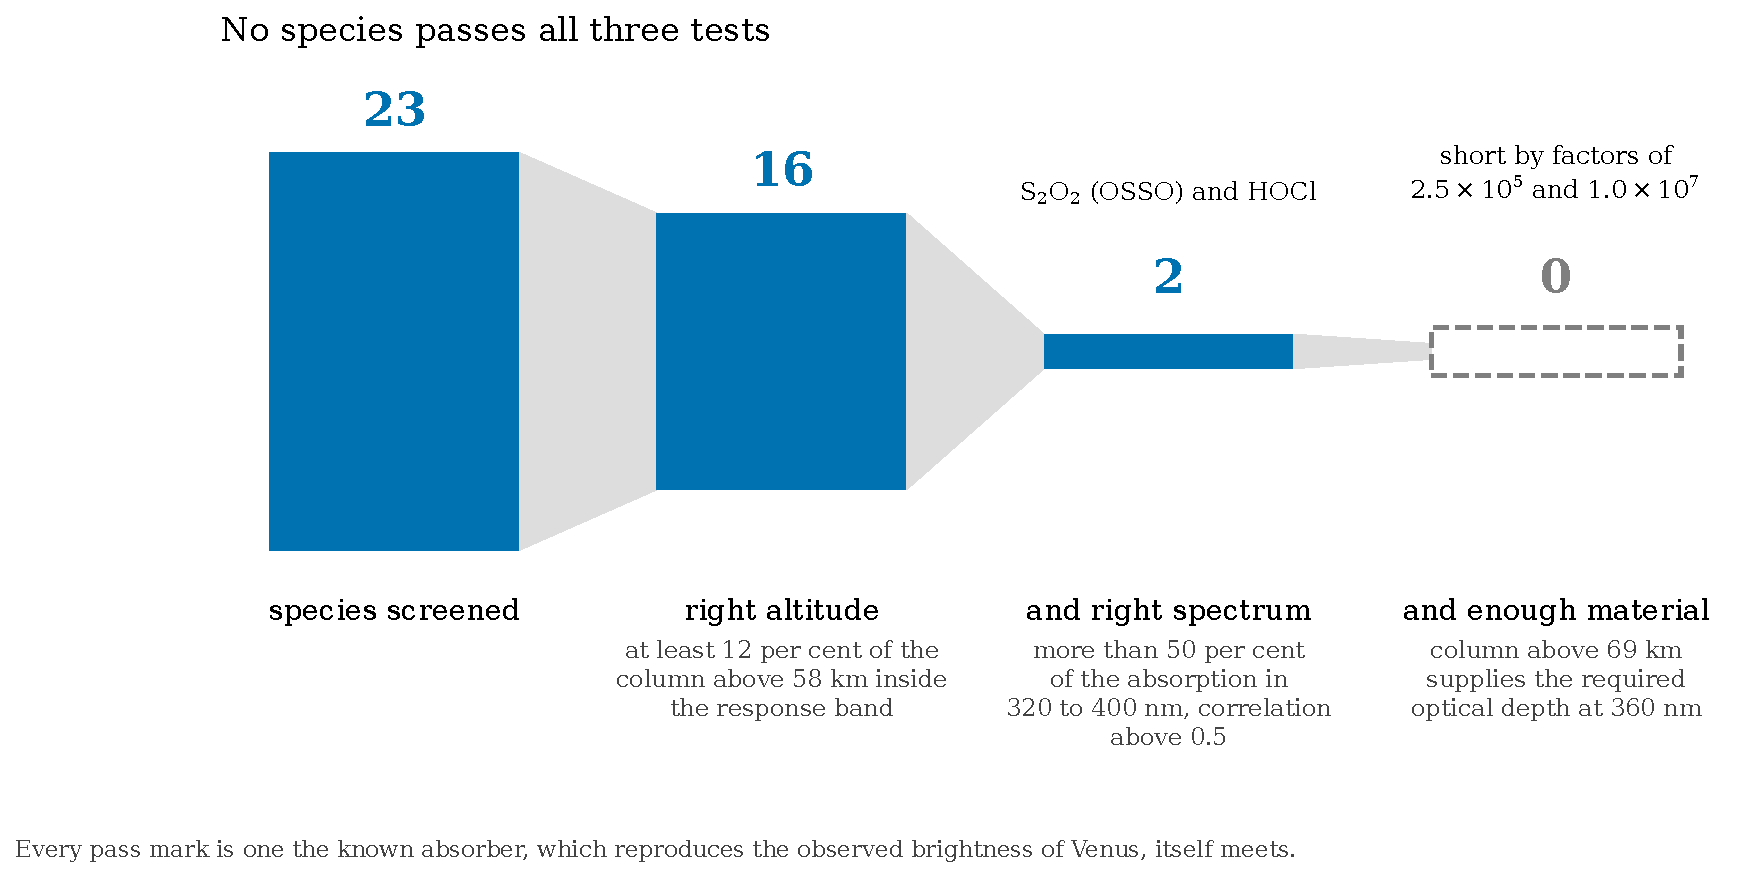
\includegraphics[width=0.92\textwidth]{F03_CTX_three-gates_ch1_backup.pdf}
  \caption[No species passes all three tests (Experiment~12)]{No species passes all three tests (Experiment~12). The 23 species the model
    can test pass through the three tests in turn; each pass mark is one the empirical
    absorber itself meets. The altitude test asks for at least the empirical absorber's
    own share of its column above 58~km inside the response band. Sources: the registry
    keys that begin \texttt{e12.gate}, which hold the counts and the pass marks, and
    \texttt{e12.S2O2.short.360} and \texttt{e12.HOCl.short.360}, which hold the two
    shortfalls. Chapter~8 explains how to read a registry key.}
  \label{fig:F3}
\end{figure}

\section{Objective and Research Gap}
\label{sec:objective}

The objective of Phase 1 was to test, inside a photochemistry and transport model, whether
the proposed carriers of the unknown absorber can meet all three requirements at once,
and to find out which of the three requirements decides the outcome. It was reached
through five steps, each of which became a group of experiments.

\textbf{Make the absorber switchable.} The model had to be able to run with the absorber
on and with it off, differing in nothing else, so that any change could be blamed on the
absorber alone (Chapter~3).

\textbf{Find where the absorber acts.} The response had to be located in amount,
wavelength, chemical reactions and altitude (Experiments~1 to~6, Chapter~5).

\textbf{Find what decides the size of the response.} Moving the absorber up or down was
compared with changing its spectrum, and the model's chemistry was then allowed to place a
candidate by itself (Experiments~7 to~10, Chapters~5 and~6).

\textbf{Test real candidates.} Published spectra and mineral data were tested against the
three requirements (Experiments~11 to~14, Chapter~6).

\textbf{Verify every number.} Every number in this report is recomputed from
the saved model output and checked automatically (Chapter~8).

\textbf{The research gap.} The studies reviewed for this project test candidates mainly on
spectral grounds, and the photochemical models among them treat the absorber either as a
fixed opacity~\cite{dai2024} or examine one candidate at a time~\cite{dai2025review,
egan2025osso}. None of them, as far as this review found, applies the amount, the altitude
and the spectrum requirements together to every species a model can represent, and none
measures how strongly the radiative effect of the absorber depends on its altitude. Phase~1
fills that gap with the following main results:
\begin{itemize}
  \item Altitude is a first-order control. Moving the absorber's profile up by
    17.8439~km changes the radiation field 7.34 times more than moving it down by
    18.0000~km (Experiment~7).
  \item The model's chemistry, not the modeller, decides where a candidate sits, and
    when it is allowed to decide, the candidate falls out of the response band
    (Experiment~9).
  \item No species the model can represent passes all three tests (Experiment~12), and
    the candidate families fail for different reasons.
  \item A published rejection of ferric chloride rests on an absorbance measured in water.
    Measured in hydrochloric acid, ferric chloride absorbs 4 to 25 times more strongly,
    and if it absorbs so in the droplets it becomes a plausible minor component
    (Experiment~14, done after Phase~1 closed). This does not identify the
    absorber.
\end{itemize}
These are negative results for the candidates tested, and they are reported as such.

\section{Organisation of this report}
\label{sec:organisation}

Chapter~2 reviews the papers this project builds on. Chapter~3 describes the model and
the groundwork that made controlled experiments possible. Chapter~4 states the
conventions used for every number. Chapters~5 and~6 describe the fourteen experiments in
the order they were done. Chapter~7 states what Phase~1 establishes and where its limits
lie. Chapter~8 describes how every number was verified and how a reader can trace any
number back to the code. Chapter~9 proposes Phase~2, and Chapter~10 concludes.


% Chapter 2. Literature Review.
% Every statement about a paper was read from the paper itself. Where a number
% is quoted, the paper is cited next to it. Critique paragraphs are marked as
% this project's own reading.

\chapter{Literature Review}
\label{ch:lit}

This chapter reviews the twelve papers on which Phase~1 rests: the model used
(Section~\ref{sec:lit-dai}); the absorber's observed spectrum and height and the mixing
in the clouds, which decide whether a candidate can sit where the absorber is
(Sections~\ref{sec:lit-ph} to~\ref{sec:lit-lef}); and the candidates, with the one paper
that states how strongly the droplets must absorb (Sections~\ref{sec:lit-jiang}
to~\ref{sec:lit-egan}). Section~\ref{sec:lit-gap} draws the threads together. For each
paper, the first part says what the authors did and how, and the second what they found,
followed by a paragraph marked as this project's own reading of what remains unsettled.

Two terms recur. A \emph{mixing ratio} is the fraction of the molecules in a volume of
air that belong to one species, in parts per million (ppmv) or per billion (ppb). The
\emph{eddy diffusion coefficient} $K_{zz}$ is the single number per height with which a
one-dimensional model represents all the vertical stirring it cannot resolve: the larger
$K_{zz}$, the faster a species is mixed up and down. It is quoted in cm$^{2}$\,s$^{-1}$
or m$^{2}$\,s$^{-1}$; one m$^{2}$\,s$^{-1}$ is $10^{4}$~cm$^{2}$\,s$^{-1}$.

% ===========================================================================
\section{Dai et al.\ (2024): the model this project uses}
\label{sec:lit-dai}

\subsection{Objective and Methodology}

Dai, Shao and Sheng built VULCAN-Venus, an open-access one-dimensional photochemistry and
transport model, to study how the chemistry depends on mixing in the clouds and on the
loss of SO\sub{2} into the droplets~\cite{dai2024}. It spans the surface to 112~km in
2~km layers, with 362 neutral and 45 photolysis reactions among 59 species, mainly from
Mills (1998) and Krasnopolsky (2007) (as cited in~\cite{dai2024}). Sunlight is followed
from 100 to 700~nm, and the droplets scatter it in two size modes. The absorber is not a
chemical species: its absorption between 320 and 560~nm is attached to the mode~1
droplets~\cite{dai2024}. The nominal $K_{zz}$, from Bierson and Zhang
(Section~\ref{sec:lit-bz}), rises from about 17\,000~cm$^{2}$\,s$^{-1}$ at the surface to
about 53\,000 at 80~km and steeply above; a case called Model~A replaces it between 46.5
and 55~km with a stronger profile from Venus Express data. Three reactions taken from
Rimmer et al.\ (Section~\ref{sec:lit-rimmer}) move SO\sub{2} into and out of the droplets
as liquid SO\sub{2}, with rates from Henry's law rather than measurement~\cite{dai2024}.

\subsection{Results and Critique}

The model reproduces the observed fall of SO\sub{2} through the clouds: SO\sub{2}
dissolves between 58 and 70~km and is released between 40 and 58~km, where the droplets
evaporate~\cite{dai2024}. Model~A changes the chemistry only slightly. OSSO reaches only
about $10^{-8}$~ppmv at 70~km, which the authors judge insufficient for the absorber; its
photolysis is omitted for lack of laboratory data~\cite{dai2024}.

\emph{This project's reading.} The absorber's amount, height and spectrum are inputs, so
the published model cannot test whether a candidate supplies them; making the absorber
switchable was the first task of this project (Chapter~3). The authors call the liquid
SO\sub{2} a ``substitute medium'' tuned to the observations~\cite{dai2024}, so SO\sub{2}
above the clouds is fitted, not predicted. The mixing test stops at 55~km, below the
cloud top where the absorber acts. And although the abstract speaks of mixing retrieved
from Venus Express, the nominal run uses the Bierson and Zhang profile.

% ===========================================================================
\section{P\'erez-Hoyos et al.\ (2018): the absorber's spectrum and height}
\label{sec:lit-ph}

\subsection{Objective and Methodology}

P\'erez-Hoyos and co-workers analysed 318 spectra from the MASCS spectrometer on
MESSENGER, taken on 5 June 2007 along the equator from near noon to the evening
terminator~\cite{perezhoyos2018}. A radiative transfer retrieval gave the height and
amount of four modes of cloud particles and the absorber's spectral shape. The absorber
was assumed well mixed with mode~1, and only the imaginary part of the mode~1 refractive
index, the part that measures absorption, was retrieved, with SO\sub{2} fixed at
500~ppb. Candidates were then ranked by how closely their spectra follow the result.

\subsection{Results and Critique}

The cloud top, where the optical depth at 0.63~\textmu m reaches one, is at $75 \pm 2$~km;
mode~1 starts at $65 \pm 2$~km with a scale height of about 4~km. The absorption is
centred at $0.34 \pm 0.03$~\textmu m with a full width at half maximum of
$0.14 \pm 0.01$~\textmu m, if Gaussian, and the data are most sensitive to it at
$75 \pm 7$~km~\cite{perezhoyos2018}. In the ranking, S\sub{2}O fits best and OSSO next,
whose shape the authors find closer; FeCl\sub{3}, SCl\sub{2} and Cl\sub{2} absorb over too
narrow a band~\cite{perezhoyos2018}. These values are the observed targets used in this
report (Figure~\ref{fig:F2}).

\emph{This project's reading.} The authors ask a candidate for the right spectrum, a
number density consistent with photochemical models, and a lifetime consistent with the
motion of the ultraviolet markings, but test only the spectrum, as they
state~\cite{perezhoyos2018}. The absorber's height is tied to mode~1 by assumption and
cannot be retrieved separately. The paper also calls the band shifted to longer
wavelengths than an earlier estimate in its results but to shorter ones in its
conclusions; this report uses only the centre and width.

% ===========================================================================
\section{Bierson and Zhang (2020): mixing and the \texorpdfstring{SO\sub{2}}{SO2} problem}
\label{sec:lit-bz}

\subsection{Objective and Methodology}

Bierson and Zhang built the first one-dimensional model to join the lower and middle
atmosphere in one domain, from the surface to 112~km, as a tool for studying how species
and regions interact rather than a tuned fit~\cite{bierson2020}. The absorber is an
imposed opacity, and water and sulfuric acid vapour are fixed because no clouds form.
They compared four $K_{zz}$ profiles: the nominal one, extended downward from an earlier
middle-atmosphere model; one from Krasnopolsky; the nominal divided by ten (Lowkzz); and
the nominal lowered to 1000~cm$^{2}$\,s$^{-1}$ between 45 and 65~km (Cloud
kzz)~\cite{bierson2020}. VULCAN-Venus adopts the nominal profile, as does every Phase~1
run (file \texttt{atm/atm\_Venus\_Bkzz.txt}).

\subsection{Results and Critique}

With the nominal profile SO\sub{2} stays almost uniformly mixed and does not fall above
the clouds~\cite{bierson2020}. Lowkzz and Cloud kzz come close, but the authors call
Lowkzz instructive for understanding the model's sensitivity rather than plausible, and
note that measured and estimated mixing in the clouds
is at least three times stronger than either. They conclude that ``some as of yet unknown
chemical sink in the cloud region or interactions with the cloud droplets'' is
needed~\cite{bierson2020}. OSSO, written (SO)\sub{2}, is below $10^{-25}$ at 58~km, never
exceeds 1~ppb, and peaks near 90~km, far above the cloud top. About 40 per cent of the
rate coefficients have no laboratory value~\cite{bierson2020}.

\emph{This project's reading.} Phase~1 uses a profile whose authors show it cannot
reproduce SO\sub{2} without an extra sink in the clouds, which Dai et al.\ supply. The
profile is published only as a figure, so its values come from the model's input file.
The verdict on OSSO rests on abundance and height, not spectrum.

% ===========================================================================
\section{Rimmer et al.\ (2021): chemistry inside the droplets}
\label{sec:lit-rimmer}

\subsection{Objective and Methodology}

Rimmer and co-workers tested three explanations for the loss of SO\sub{2} and water in
and above the clouds: more water below the clouds, less SO\sub{2} below them, and
chemistry inside the droplets enabled by dissolved hydroxide salts, with sodium hydroxide
as a stand-in~\cite{rimmer2021}. In their 480 species model, gas dissolves into the
droplets by Henry's law and the salts neutralise part of the acid so that more SO\sub{2}
is held. The absorber is a fixed optical depth between 58 and 67~km, fading above.

\subsection{Results and Critique}

Without extra hydrogen, the water available removes only about 20 per cent of the
SO\sub{2}~\cite{rimmer2021}. More water fails, raising the cloud top 20~km too high and
the oxygen far too much. Less SO\sub{2} below the clouds works at 15 to 20~ppm (the paper
gives both), against about 150~ppm observed. Salts reproduce SO\sub{2} with a droplet pH
of about 1 at 50~km, but need a continuous supply of about
$10^{-13}$~mol\,cm$^{-2}$\,s$^{-1}$, some four orders of magnitude more than delivery
from space~\cite{rimmer2021}. No gas in their models explains the absorber above 200~nm,
and the particles' own absorption was not considered.

\emph{This project's reading.} The salt profile is prescribed at each height to fit
SO\sub{2}, its source lies outside the mass balance, and the authors call the solution not
unique~\cite{rimmer2021}. The paper shows that buffered droplets \emph{could} hold the
missing SO\sub{2}, not that a real salt reaches them. Dai et al.\ adopted its droplet
reaction rates.

% ===========================================================================
\section{Lef\`evre et al.\ (2022, 2024): resolved convection in the clouds}
\label{sec:lit-lef}

\subsection{Objective and Methodology}

Lef\`evre and co-workers measured $K_{zz}$ instead of assuming it, with a large-eddy
simulation: a three-dimensional model fine enough to resolve single rising plumes, with a
400~m grid over a box 64~km wide, from the surface to 90~km~\cite{lefevre2022}. The 2022
study followed idealised tracers for SO\sub{2} and water at the equator and at 75 degrees
latitude at noon, and derived $K_{zz}$ from their simulated vertical fluxes. The 2024
study added full photochemistry, equilibrium clouds and midnight, and derived an
effective $K_{zz}$ for each species~\cite{lefevre2024}. The solar heating corresponds to
a fixed, average amount of absorber~\cite{lefevre2022}.

\subsection{Results and Critique}

A deep convective layer sits at about 47 to 56~km at the equator. There, at noon, a cloud-top
convective layer appears at about 66 to 74~km, driven by the absorber's own solar
heating; it is absent at night and at high latitude, and the authors call it still
speculative~\cite{lefevre2022}. The effective $K_{zz}$ in the deep layer is about
$10^{3}$~m$^{2}$\,s$^{-1}$ for SO\sub{2} and $10^{2}$ for water; in the cloud-top layer it
rises from about 1~m$^{2}$\,s$^{-1}$ at 65~km to $10^{4}$ at 72~km, raising SO\sub{2} at
72~km from 0.17 to 0.7~ppm~\cite{lefevre2024}. These values are orders of magnitude above
those in one-dimensional chemistry models~\cite{lefevre2024}, none of which yet includes
the cloud-top convection~\cite{lefevre2022}.

\emph{This project's reading.} Neither paper moves or changes the absorber, though the
2022 paper says its uncertain abundance ``could have a strong effect'' on the cloud-top
convection~\cite{lefevre2022}. Absorber and mixing are coupled: the heating drives mixing
that redistributes the absorber. Neither paper reports mixing above about 75~km, leaving
most of this project's 69 to 93~km response band (Chapter~5) unconstrained, and the
species-dependent $K_{zz}$ shows that VULCAN-Venus's single $K_{zz}$ is a simplification.
These points motivate Phase~2 (Chapter~9).

% ===========================================================================
\section{Jiang et al.\ (2024): iron sulfate minerals}
\label{sec:lit-jiang}

\subsection{Objective and Methodology}

Jiang and co-workers tested in the laboratory which iron sulfate minerals survive in
sulfuric acid of droplet strength, and whether their absorption matches the
absorber~\cite{jiang2024}. Minerals were kept in 50 to 98 weight per cent acid for up to
30 days at room temperature and 1~bar and followed by Raman spectroscopy. The absorbance
of the surviving minerals and of dissolved iron, normalised to a maximum of one between
200 and 500~nm, was fitted to the observed spectrum.

\subsection{Results and Critique}

Rhomboclase is stable up to 74.2~wt\% acid and becomes acid ferric sulfate in stronger
acid: within 14 days at 79.1~wt\%, two hours at 83.5~wt\% and five minutes at
97.4~wt\%~\cite{jiang2024}. The best fit mixes 1~wt\% rhomboclase in 74.2~wt\% acid with
1.25~wt\% acid ferric sulfate in 83.5~wt\% acid; dissolved iron matches 200 to 300~nm.
The authors estimate that about 1 to 2~wt\% of absorber is needed, against at most
$10^{-3}$~wt\% iron from
generous estimates of delivery from space, and that rhomboclase forms only where the
droplets are out of equilibrium or in balance with about 100~ppm or more of water vapour,
above the 30~ppm observed below the clouds~\cite{jiang2024}.

\emph{This project's reading.} Normalised spectra test shape, not strength; the absolute
coefficients are in the supplementary material, which Experiment~13 uses (Chapter~6).
Nothing is modelled about transport, settling or chemistry, so whether the minerals stay
at the cloud top, and how the iron arrives, is untested. Dai et al.\ note that the
minerals formed under a particular laboratory setting, not a Venus-like
one~\cite{dai2024}.

% ===========================================================================
\section{Trabelsi and Francisco (2026): chlorine and sulfur molecules}
\label{sec:lit-trabelsi}

\subsection{Objective and Methodology}

Trabelsi and Francisco calculated from first principles the structure, vibrations,
excited states and cross sections from 200 to 600~nm of three forms of
S\sub{2}Cl\sub{2} (ClSSCl, SSCl\sub{2} and a ring form), as isolated gas molecules at
absolute zero~\cite{trabelsi2026}.

\subsection{Results and Critique}

ClSSCl absorbs strongly near 240~nm, against a measured band near 256 to 260~nm.
SSCl\sub{2} absorbs from about 410~nm, with maxima near 348 and 262~nm, and since this
overlaps the absorber's range the authors conclude it ``could
contribute''~\cite{trabelsi2026}. They offer the results as better inputs for
photochemical models.

\emph{This project's reading.} The paper gives spectra, not amounts: no abundance,
production, lifetime or altitude. A molecule that absorbs in the near ultraviolet is also
broken up by it, so it would need a continuous source. The authors supplied their cross
sections, which Experiment~11 runs in the model (Chapter~6).

% ===========================================================================
\section{Egan et al.\ (2025): OSSO tested end to end}
\label{sec:lit-osso}

\subsection{Objective and Methodology}

Egan and co-workers asked whether OSSO can be abundant enough~\cite{egan2025osso}. They
computed new rate coefficients for its formation from two SO molecules and for its loss,
placed them in a three-dimensional model of the whole atmosphere with a sulfur source from
meteors, ran it for nine Venus days to a steady state, and compared the resulting
reflectance, from a radiative transfer model, with the MESSENGER spectrum.

\subsection{Results and Critique}

OSSO forms a thin layer near 70~km, about three orders of magnitude short of the observed
absorption, still two orders short with its loss to oxygen and chlorine atoms switched
off, and with too narrow a band~\cite{egan2025osso}. SO\sub{2} above the clouds was kept
deliberately too high, which favours OSSO, and the authors conclude that OSSO does not
contribute significantly.

\emph{This project's reading.} This is the only peer-reviewed paper reviewed here in which
the chemistry sets a candidate's amount and the reflectance follows from it, and so the
only independent check on this
project's screen, which reaches the same verdict against a different yardstick
(Experiment~12, Chapter~6). Its radiative step uses one column at the equator near
midday, and its loss rates are calculated, not measured.

% ===========================================================================
\section{Spacek et al.\ (2026): how strongly the droplets must absorb}
\label{sec:lit-spacek}

\subsection{Objective and Methodology}

Spacek, Rimmer, Petkowski and Lee asked how strongly the droplet liquid must absorb, in
units a laboratory measures~\cite{spacek2026}. They fitted a multiple scattering model to
dayside reflectance between 365 and 455~nm from a 2020 campaign, with the absorber spread
evenly through mode~1 and mode~2 droplets between 59 and 65~km and represented by a
lowered \emph{single scattering albedo}, the fraction of light meeting a particle that
is scattered rather than absorbed. The absorption per unit droplet volume gives the
\emph{decadic absorption coefficient} $a$ of the liquid: the absorbance of a 1~cm path
in a laboratory cell.

\subsection{Results and Critique}

The single scattering albedo must be 0.89 at 365~nm, and $a$ peaks at 1278~cm$^{-1}$ at
375~nm, falling below 54~cm$^{-1}$ at 455~nm~\cite{spacek2026}. An efficient organic
absorber would have to make up about 0.5 to 7 per cent of the droplet liquid, nearly four
orders of magnitude above the authors' estimate of the organic carbon available; weaker
inorganic absorbers would have to be a major part of the droplets. Ferric chloride is
rejected because 1~g per litre of \emph{water} gives about 1~cm$^{-1}$ at 375~nm, so a
straight-line extrapolation needs about 1.3~kg per litre~\cite{spacek2026}.

\emph{This project's reading.} The requirement holds only for the assumed layer, mixing
and droplet sizes, as the authors acknowledge. The ferric chloride figure rests on a
measurement in water, though the same paper warns that aqueous spectra have limited value
unless Venus conditions are reproduced~\cite{spacek2026}, and it cites the sulfuric acid
measurements of Egan et al.\ only for spectral shape. Experiment~14, done after Phase~1
closed, repeats the calculation with the same group's measurements of ferric chloride in
hydrochloric acid (Section~\ref{sec:lit-egan} and Chapter~6).

% ===========================================================================
\section{Egan et al.\ (2025, 2026): ferric chloride in sulfuric acid}
\label{sec:lit-egan}

\subsection{Objective and Methodology}

The ferric chloride spectrum used in recent comparisons had been measured in an organic
solvent with which it can react~\cite{egan2025lab}. Egan, James and Plane measured it
from 200 to 600~nm in about 77 and 78~wt\% sulfuric acid with added hydrochloric acid, at
room temperature, and followed its slow conversion to ferric sulfate for about a hundred
days~\cite{egan2025lab}. To fit these mixtures they also derived its molar absorptivity
in hydrochloric acid of several strengths (their Figure~5a), the curves Experiment~14
uses~\cite{egan2025lab}. A preprint by the same group, posted on 14 January 2026 and
marked as not peer reviewed~\cite{egan2026}, added 57 iron reactions to a
three-dimensional model of Venus, with iron from meteors and chlorine from atmospheric
hydrogen chloride, and used the laboratory spectra in a radiative transfer model compared
with the MESSENGER spectrum.

\subsection{Results and Critique}

Ferric chloride had not been measured in concentrated sulfuric acid before, the solvent
has a significant effect on its spectrum, and hydrochloric acid slows its conversion to
sulfate~\cite{egan2025lab}. Its normalised shape agrees well with the absorber, but the
authors add that altitude, formation, lifetime and transport ``must all be considered
through extensive atmospheric modeling'' first. The preprint finds that 1.0 to 1.2~wt\%
ferric chloride in mode~1 droplets reproduces the absorption between 300 and 600~nm (1.2
to 1.5~wt\% if part turns to sulfate), and that a purely meteoric source needs the iron to
stay in the clouds for about 3000 years~\cite{egan2026}.

\emph{This project's reading.} The laboratory spectra were taken several hundred to about
a thousand times more dilute than the fitted loadings, so using them at those loadings
assumes that absorbance grows in proportion to the amount. In the
preprint the amount comes from the radiative fit, not the chemistry, whose run had not
reached a steady state, and the residence time is 2800 and 3400 years in the discussion
but 1800 to 3000 in the conclusions~\cite{egan2026}. Most important here, Spacek et al.\
and the preprint reach opposite conclusions on ferric chloride and neither cites the
other. Experiment~14 (Chapter~6) traces the disagreement to the solvent of the input
measurement; it does not identify the absorber.

% ===========================================================================
\section{What the literature leaves open}
\label{sec:lit-gap}

Against the three tests of Section~\ref{sec:question}, the coverage is uneven.
\textbf{The spectrum} is tested most often, almost always as a normalised shape.
\textbf{The amount} has been tested for a few candidates, one at a time, and only Spacek
et al.\ state the absolute strength the droplets need. \textbf{The altitude} is assumed:
tied to mode~1, set as a fixed layer, or prescribed. No paper reviewed lets a chemistry
model place a candidate by itself and then measures how the radiation responds to where
it sits, while the mixing that would carry a candidate there is uncertain by orders of
magnitude and may be driven, at the cloud top, by the absorber itself. This is the gap of
Section~\ref{sec:objective}, and the following chapters describe how Phase~1 addressed it.

% Chapter 3. The Model and the Groundwork.
% Model numbers come from verify/registry.json (keys named in the text), from
% vulcan_cfg.py, or from the committed input files named next to them.

\chapter{The Model and the Groundwork}
\label{ch:model}

Before any experiment could be run, three things had to exist: a model whose working
was understood, a baseline run that could be trusted, and a way to switch the absorber
on and off while changing nothing else. This chapter explains how a photochemistry and
transport model works (Section~\ref{sec:how}), describes VULCAN-Venus as it is used here
(Section~\ref{sec:vulcan}), and then tells the groundwork in the order it happened: the
environment and baseline (Section~\ref{sec:baseline}), a false lead
(Section~\ref{sec:falselead}), the discovery that made controlled experiments possible
(Section~\ref{sec:discovery}), and the requirement every candidate is later measured
against (Section~\ref{sec:taureq}). Section~\ref{sec:plan} shows how the experiments
grew from it.

% ===========================================================================
\section{How a photochemistry and transport model works}
\label{sec:how}

The model treats the atmosphere as a column of horizontal layers, the same everywhere
around the planet, so that only height varies; this is what \emph{one-dimensional}
means. In each layer it follows the number density $n_i$ of every species $i$, the
number of its molecules per cubic centimetre. The density changes for two reasons:
chemistry makes or destroys the species, and mixing carries it between layers. The
model solves, for every species and every layer,
\begin{equation}
  \frac{\partial n_i}{\partial t} = P_i - L_i - \frac{\partial \phi_i}{\partial z},
  \label{eq:continuity}
\end{equation}
where $t$ is time, $z$ is altitude, $P_i$ and $L_i$ are the rates at which reactions
produce and destroy species~$i$ (molecules per cubic centimetre per second), and
$\phi_i$ is its upward flux (molecules per square centimetre per second). The flux is
given by eddy diffusion,
\begin{equation}
  \phi_i = -K_{zz}\, n \,\frac{\partial X_i}{\partial z},
  \label{eq:flux}
\end{equation}
where $n$ is the total number density of the air, $X_i = n_i/n$ is the mixing ratio of
species~$i$, and $K_{zz}$ is the eddy diffusion coefficient of Chapter~\ref{ch:lit}. The
minus sign makes a species flow from where its mixing ratio is high to where it is low.

Many reactions are driven by sunlight. A molecule that absorbs a photon of enough
energy can break apart; this is \emph{photolysis}. How much sunlight reaches a layer
depends on how much has been absorbed or scattered above it, measured by the optical
depth. At the lower boundary of layer $j$ and wavelength $\lambda$ the model adds up
that layer and every layer above it:
\begin{equation}
  \tau(j,\lambda) = \sum_{k \ge j} \Big[ \sum_{s} n_s(k)\,\sigma_s(\lambda) \Big]\,
  \Delta z_k ,
  \label{eq:tau}
\end{equation}
where $n_s(k)$ is the number density of absorbing or scattering species $s$ in layer
$k$, $\sigma_s(\lambda)$ is its cross section, the effective area one molecule presents
to light (square centimetres), and $\Delta z_k$ is the layer thickness in centimetres.
Sunlight arriving from a direction at angle $\theta$ to the vertical is weakened in
proportion to $e^{-\tau/\cos\theta}$. The model then computes the \emph{actinic flux}
$F(z,\lambda)$, the number of photons per square centimetre per second per nanometre
arriving at a point from all directions, including light scattered by the gas. The rate
coefficient of a photolysis reaction of species $s$ is
\begin{equation}
  J_s(z) = \int \sigma_s(\lambda)\, q_s(\lambda)\, F(z,\lambda)\, \mathrm{d}\lambda ,
  \label{eq:J}
\end{equation}
where $q_s(\lambda)$ is the fraction of absorbed photons that break the molecule, so that
$J_s$ is the probability per second that one molecule is broken up. The destruction rate
it contributes to $L_s$ is $J_s n_s$, halved in this model for day and night
(Table~\ref{tab:setup}).

These equations are coupled. An absorber in a high layer raises $\tau$ below it, which
lowers $F$, which lowers every $J$, which changes the chemistry, which changes the
abundances that set $\tau$. This chain, from optical depth to actinic flux to photolysis
to chemistry, is the path by which the unknown absorber can affect the model at all.

The model is integrated in time until it no longer changes, which is called
\emph{steady state}. VULCAN-Venus declares steady state when three tests pass at once:
the largest fractional change of any mixing ratio over the recent steps, called
\texttt{longdy}, is below 0.01; that change divided by the elapsed time,
\texttt{longdydt}, is below $10^{-5}$ per second; and the largest fractional change of
the actinic flux from one step to the next is below 0.1 (\texttt{yconv\_cri},
\texttt{slope\_cri} and \texttt{flux\_cri} in \texttt{vulcan\_cfg.py}, tested in
\texttt{op.py}).

% ===========================================================================
\section{VULCAN-Venus as used in this project}
\label{sec:vulcan}

VULCAN is a general photochemistry and transport model; VULCAN-Venus is its adaptation
to Venus by Dai, Shao and Sheng~\cite{dai2024}, reviewed in Section~\ref{sec:lit-dai}.
Table~\ref{tab:setup} lists the settings of every Phase~1 run.

\begin{table}[htbp]
  \centering
  \caption[The model set-up used in every Phase~1 run]{The model set-up used in every Phase~1 run. Configuration lines are in
    \texttt{vulcan\_cfg.py}; counts from saved output are in the registry under the keys
    shown.}
  \label{tab:setup}
  \footnotesize
  \setstretch{1.0}
  \begin{tabularx}{\textwidth}{>{\raggedright\arraybackslash}p{3.1cm}
                                >{\raggedright\arraybackslash}X
                                >{\raggedright\arraybackslash}p{4.7cm}}
    \toprule
    Property & Value & Source \\
    \midrule
    Vertical grid & 0 to 112~km in 57 layers: 56 layers 2~km thick and a vanishingly thin
      layer at the surface & \texttt{atm/alt\_venus.txt} \\
    Temperature and pressure & 733~K and about 92~bar at the surface (the model's own
      profile, a little cooler than the 750~K of Chapter~\ref{ch:intro}); about one
      millionth of a bar at the top & \texttt{atm/atm\_Venus\_Bkzz.txt} \\
    Eddy diffusion & Bierson and Zhang nominal profile~\cite{bierson2020} &
      \texttt{atm/atm\_Venus\_Bkzz.txt} \\
    Chemistry & Network \texttt{Nominal.txt}: 62 entries in the species list, 838 reaction
      slots (a forward and a reverse slot per reaction) & \texttt{nom.base.v.nr} \\
    Wavelength grid & 1670 bins, 96 to 698~nm; 0.1~nm wide below 240~nm, 2~nm above &
      \texttt{nom.base.v.nbin}, \texttt{.dbin1}, \texttt{.dbin2} \\
    Sunlight & One zenith angle of 58 degrees, the dayside average; every photolysis rate
      halved for the day and night average & \texttt{sl\_angle}, \texttt{f\_diurnal} \\
    Fixed surface mixing ratios & SO\sub{2} 100~ppmv, COS 30~ppmv, CO 15~ppmv, among
      others & \texttt{use\_fix\_sp\_bot} \\
    Fixed profiles & H\sub{2}SO\sub{4} vapour and liquid, water vapour and condensed
      water, N\sub{2}, and the two particle tracers & \texttt{fix\_species} \\
    Switched off & Vertical wind, molecular diffusion & \texttt{use\_vz},
      \texttt{use\_moldiff} \\
    Absorber input & $Q_{\mathrm{abs}}(\lambda)$ table; mode~1 particle profile &
      \texttt{atm/UV\_absorber.txt}, \texttt{atm/mode1+2.txt} \\
    \bottomrule
  \end{tabularx}
\end{table}

Three features of this set-up matter for what follows. First, the column is a single
global average at one sun angle, so day and night, latitude and season are not
represented. Second, the sulfuric acid and water that make up the clouds are fixed
profiles; the model does not form or move cloud droplets. Third, as
Section~\ref{sec:discovery} explains, the radiation in the code as supplied included gas
absorption, scattering by molecules and the cloud droplets in a simplified form, but
not the absorber.

% ===========================================================================
\section{The environment and the baseline}
\label{sec:baseline}

Work began by building a working environment, Ubuntu 24.04 running under WSL2 on Windows
with a Conda environment named \texttt{venus}, as recorded in
\texttt{documentation/SETUP\_AND\_REPRODUCTION.md}. The supplied code predates the
current Python libraries, and two small compatibility corrections were needed: one line
in \texttt{make\_chem\_funs.py} that assumed text arrives as raw bytes, and one import in
the PyMieScatt library whose function had been renamed in SciPy. Neither changes any
chemical, atmospheric or optical input.

The order of the next two steps mattered. The output file supplied with the model was
first copied and checked to be identical, byte for byte, to the original; this copy is
called the \emph{reference}. Only then was the model run afresh, giving the
\emph{baseline}. Without a preserved reference, no later disagreement could have been
pinned on anything. Both runs met the steady-state tests of Section~\ref{sec:how}.
The baseline needed 296 steps and reached a model time of
$5.328\times10^{8}$~s, with \texttt{longdy} equal to 0.0099016 and \texttt{longdydt}
equal to $6.971\times10^{-11}$~s$^{-1}$; the reference had been integrated much longer,
over 14336 steps to $3.082\times10^{10}$~s, and ended at 0.0097880 and
$7.219\times10^{-11}$~s$^{-1}$ (registry keys beginning \texttt{nom.base} and
\texttt{nom.ref}).

The two states were then compared quantity by quantity: mixing ratios, optical depth,
actinic flux and photolysis rates. The grid, pressure, temperature, layer thickness,
$K_{zz}$ and cross sections were identical. The states agreed closely almost everywhere,
with one exception.

% ===========================================================================
\section{A false lead: the 200 to 220 nm anomaly}
\label{sec:falselead}

Around 54 to 58~km and between about 200 and 220~nm, the optical depth of the two states
differed sharply. At 54~km (grid interface 28) and 201.6~nm, the
reference optical depth is 1376.448 and the baseline 933.950, a difference of 442.498
(registry keys beginning \texttt{falselead}).

This looked, briefly, like a signal: it was in the ultraviolet and inside the clouds. It
would have been easy to take it as a trace of the absorber. It was traced instead. Since
all inputs were identical, the difference had to come from the computed composition. In
layer 28 the SO\sub{2} mixing ratio differs by about a third between the two states, and
recomputing Equation~\eqref{eq:tau} from the two SO\sub{2} profiles alone reproduces
essentially the whole optical depth difference at that point. Going one step further
back, gas-phase sulfuric acid and SO\sub{3} in that layer are about fourteen times lower
in the baseline, while the fixed liquid sulfuric acid is identical. The reference had been integrated nearly sixty times longer than the baseline. The chain
therefore runs from a difference in sulfur chemistry between the two states to
SO\sub{2}, and from SO\sub{2} to optical depth, where SO\sub{2} absorbs strongly.

This conclusion was reached before any experiment was run: the 200 to 220~nm anomaly is
a difference between two model states caused by ordinary SO\sub{2} absorption, and it
must not be used as evidence of the absorber. Rejecting it kept the control of every
later experiment clean.

% ===========================================================================
\section{The discovery: an absorber term that was switched off}
\label{sec:discovery}

The absorber was then audited directly in the source code. The code reads the absorber
table, a list of absorption efficiencies $Q_{\mathrm{abs}}(\lambda)$, interpolates it onto
the model's wavelength grid, takes the absorbing particles to be the mode~1 droplets with
diameter $D = 0.98$~\textmu m, and takes their number density from the mode~1 profile.
From these it forms, for each layer $j$, the absorber's share of the optical depth,
\begin{equation}
  \tau_{\mathrm{UUV}}(j,\lambda)
    = Q_{\mathrm{abs}}(\lambda)\,\frac{\pi D^{2}}{4}\,N(j)\,\Delta z_j ,
  \label{eq:tauuuv}
\end{equation}
where $\pi D^{2}/4$ is the cross-sectional area of one particle, $N(j)$ is the number of
particles per cubic centimetre in layer $j$, and $\Delta z_j$ is the layer thickness in
centimetres. $Q_{\mathrm{abs}}$ is the fraction of light falling on that area that the
particle absorbs. The subscript UUV, for \emph{unknown ultraviolet}, is the name the code
uses.

The decisive finding was that this calculation, together with a full scattering
calculation for the two modes of cloud droplets, sat inside a block of code that had been
turned into a comment, in the function \texttt{compute\_tau()} of \texttt{op.py}. It was
present but never executed. The comment beside it says why: the droplet calculation had
been replaced by fixed, fitted cross sections for the two droplet modes, carried as two
particle species named \texttt{V} and \texttt{V2}, to save computation. The optical depth
the supplied code actually computed was therefore gas absorption, scattering by
molecules and these two droplet species, and the saved output held no absorber arrays.
Recomputing the saved optical depth from those terms matched it to very small numerical
residuals.

This is what made the project possible. Because the term existed, it could be switched on
under a single number, the amplitude $A_{\mathrm{UUV}}$:
\begin{equation}
  \tau^{*}_{\mathrm{UUV}} = A_{\mathrm{UUV}}\;\tau_{\mathrm{UUV}} .
  \label{eq:amp}
\end{equation}
With $A_{\mathrm{UUV}} = 0$ the model is exactly as supplied, which is the
\emph{control}. With $A_{\mathrm{UUV}} = 1$ it carries the supplied absorber exactly as
tabulated, which is the \emph{treatment}. The two runs differ in one term and in nothing
else, so any difference between them can be blamed on the absorber alone, through the
chain of Section~\ref{sec:how}. Only this term was switched on; the full droplet calculation
stayed off, and the droplets enter every run, control and treatment alike, through the
same fitted cross sections, so that the comparison isolates the absorber. The source file was
copied before the change and the copy checked identical by its SHA-256 hash (\texttt{op-25m0328-pre-UUV-experiment.py}),
and the amplitude is set in \texttt{vulcan\_cfg.py} as \texttt{A\_UUV}.

\textbf{The absorber as supplied.} The absorber that comes with the model, called the
\emph{empirical absorber} in this report, has two parts, and every later experiment
changes one or both of them. Its \emph{spectrum} is the table of $Q_{\mathrm{abs}}$ in
\texttt{atm/UV\_absorber.txt}. It is non-zero from 302 to 698~nm
(\texttt{spec\_emp.sup\_lo} and \texttt{.sup\_hi}), largest at 320~nm, where it is 0.356
(\texttt{spec\_emp.peakQ}), and 61.58\% of its absorption lies between 320 and 400~nm
(\texttt{share320400.emp}). Its \emph{profile} is the mode~1 particle density in
\texttt{atm/mode1+2.txt}. The density is largest at 60~km, with 595 particles per cubic
centimetre (\texttt{pnom.peak\_z} and \texttt{pnom.peak\_N}); the profile is centred at
63.419~km (\texttt{pnom.centroid}), holds 90.194\% of its particles between 58 and 69~km
(\texttt{pnom.p5869}) and none below 30~km, and adds up to $4.0776\times10^{8}$ particles
per square centimetre over the whole column (\texttt{pnom.column}). Experiment~7 moves the
profile and keeps the spectrum; Experiments~8 and~11 change the spectrum and keep the
profile; Experiments~9 and~10 change both.

% ===========================================================================
\section{The requirement constant}
\label{sec:taureq}

Adding Equation~\eqref{eq:tauuuv} over every layer gives the absorber's optical depth
through the whole atmosphere, which is the amount of absorption any real candidate must
supply. It is largest at 320~nm, where the table peaks:
\begin{equation}
  \tau_{\mathrm{req}} = Q_{\mathrm{abs}}(320~\mathrm{nm})\,\frac{\pi D^{2}}{4}
    \sum_{j} N(j)\,\Delta z_j = 1.094968472081 .
  \label{eq:taureq}
\end{equation}
Here $Q_{\mathrm{abs}}(320~\mathrm{nm}) = 0.356$ (registry key
\texttt{spec\_emp.peakQ}), the particle area is $7.543\times10^{-9}$~cm$^{2}$
(\texttt{const.area}), and the column of mode~1 particles is
$4.0776\times10^{8}$ per square centimetre (\texttt{pnom.column}). The result is held
as \texttt{const.tau\_req}. It is the same in the reference and the baseline, as it must
be, because it depends only on input tables.

In plain terms, sunlight at 320~nm that passes straight down through the absorber layer
keeps a fraction $e^{-\tau_{\mathrm{req}}}$ of its intensity, about one third. Because this number was recovered from the model's own inputs rather than taken
from a paper, every candidate in Chapter~6 is measured against exactly the absorption the
model's own absorber supplies. When the model was run with the absorber switched on, its
optical depth at 56~km, below the absorber, exceeded that of the control by this same
amount at 320~nm, as expected.

% ===========================================================================
\section{From groundwork to experiments}
\label{sec:plan}

With a trusted baseline and a clean control, the experiments followed in four stages,
shown in Figure~\ref{fig:F4}. Experiments~1 and~2 switch the absorber on and ask whether,
and what, it changes. Experiments~3 to~6 locate the response in amount, wavelength,
reaction and altitude. Experiments~7 to~10 ask what decides the size of the response, and
Experiments~11 to~14 test real candidates against what the earlier stages found.
Chapter~4 first states the conventions used for every number, and Chapters~5 and~6
describe the experiments in the order they were done.

\begin{figure}[htbp]
  \centering
  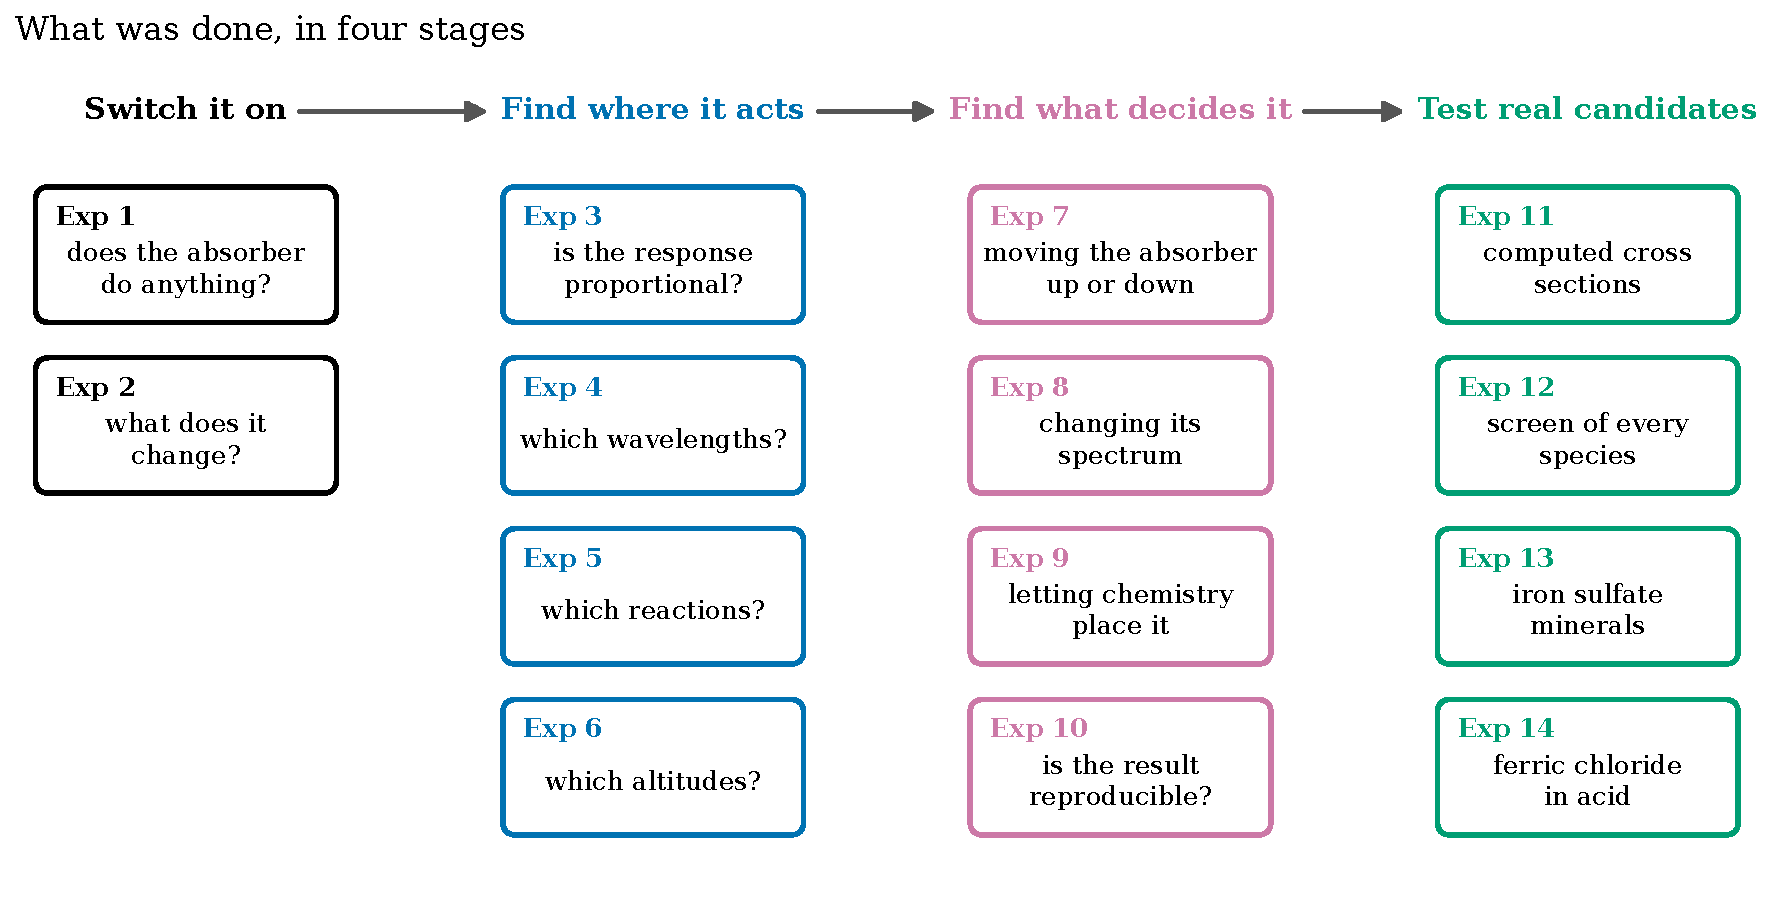
\includegraphics[width=\textwidth]{F04_CTX_what-was-done_ch3_report.pdf}
  \caption[What was done, in four stages]{What was done, in four stages. Each box is one experiment and the question it
    asked, and each stage builds on what the stage before it found. Source:
    \texttt{figures/scripts/F04\_CTX\_what-was-done.py}.}
  \label{fig:F4}
\end{figure}

% Chapter 4. Method and Conventions.
% Every number in this chapter comes from verify/registry.json (keys named in the
% text), from verify/recompute_25m0328.py, or from the committed model output.

\chapter{Method and Conventions}
\label{ch:conv}

Every experiment in Chapters~5 and~6 compares two converged model states and reports
how they differ. A difference can be measured in more than one way, and two honest
calculations from the same output can give different numbers if they make different
choices. This chapter states every choice that was made, so that a reader who repeats
a calculation gets the number printed here: how numbers are written
(Section~\ref{sec:conv-numbers}), the six conventions with a worked example each
(Section~\ref{sec:conv-six}), the fixed ranges used throughout
(Section~\ref{sec:conv-windows}), how the size of a change in the whole radiation field
is measured (Section~\ref{sec:conv-field}), the response band
(Section~\ref{sec:conv-band}) and the reproducibility floor
(Section~\ref{sec:conv-floor}).

The same six conventions are also written out in the code that computes every number,
\texttt{verify/recompute\_25m0328.py}: the first five at the top of the file, and the
sixth as the value of the key \texttt{res.e10.SO.inband}. Where a recomputation disagrees with a number in
this report, the first thing to check is whether it follows these conventions.

% ===========================================================================
\section{How numbers are written in this report}
\label{sec:conv-numbers}

The registry, the file \texttt{verify/registry.json}, holds every quantity computed from
the model, each under its own name, called a \emph{registry key}; an example is
\texttt{e6.A1.meanz}. Chapter~8 explains how to read these names. Where this report prints such a number, the key is
named next to it or at the start of the paragraph.

A printed number carries only as many digits as the text needs. It is correct when the
registry value, rounded to the same number of significant digits, gives the printed
number. For example, \texttt{e6.A1.meanz} holds the response centroid to sixteen digits,
and the text prints it as 82.044~km. The project's checker,
\texttt{verify/check\_documents\_25m0328.py}, applies this rule against the whole
registry to every number written with three or more decimal places, in scientific
notation, or as a percentage with two or more decimal places.
Percentages may be stored either as percentages or as fractions; 1.4484\% and a stored
0.014484 are the same number.

The checker can show that a printed number exists in the registry. It cannot show that it
was taken from the right key. That second check is done by hand, by recomputing the
sentence from the key it names, and Chapter~8 gives an example where it mattered.

% ===========================================================================
\section{The six conventions}
\label{sec:conv-six}

Table~\ref{tab:conventions} lists the six conventions. Each is explained below with a
worked example.

\begin{table}[htbp]
  \centering
  \caption[The six conventions used for every number in this report]{The six conventions used for every number in this report.}
  \label{tab:conventions}
  \footnotesize
  \setstretch{1.0}
  \begin{tabularx}{\textwidth}{>{\raggedright\arraybackslash}p{0.7cm}
                                >{\raggedright\arraybackslash}p{4.2cm}
                                >{\raggedright\arraybackslash}X}
    \toprule
    No. & Convention & What it means \\
    \midrule
    1 & Relative change & The difference is divided by the larger of the two values,
      not by the control. \\
    2 & Means over a field & Every element counts equally. A \emph{bounded} mean
      leaves out the elements where both values are zero. \\
    3 & Integrals over wavelength & VULCAN's own rule: two bin widths, and half weight
      at the two ends of every range. \\
    4 & Integrals over altitude & Layer thickness in centimetres, never kilometres. \\
    5 & Two photolysis measures & $\Delta J$ (the rate coefficient) and $\Delta(J n)$
      (the rate) are different quantities and are never mixed. \\
    6 & Reproducibility floor & In-band changes in abundance smaller than 2.5278\% are
      not resolved. \\
    \bottomrule
  \end{tabularx}
\end{table}

% ===========================================================================
\subsection{Relative change divides by the larger value}
\label{sec:conv-rel}

When a quantity $X$ has the value $X_{\mathrm{r}}$ in the reference run and
$X_{\mathrm{c}}$ in the case being tested, its relative change is
\begin{equation}
  R_X = \frac{|X_{\mathrm{c}} - X_{\mathrm{r}}|}
             {\max\big(|X_{\mathrm{r}}|,\,|X_{\mathrm{c}}|\big)} .
  \label{eq:rel}
\end{equation}
The denominator is the larger of the two magnitudes. This keeps $R_X$ between 0 and 1,
or between 0 and 100 per cent, whatever the two values are, and it is defined even when
the reference value is zero. For a small change the larger value and the reference
value are almost equal, and the two possible definitions agree. They differ only when
the change is large, which is exactly where a percentage needs care.

\textbf{Worked example.} In Experiment~2 the mixing ratio of OSSO (S\sub{2}O\sub{2}) at
33~km rises from $4.012\times10^{-42}$ with the absorber off to $3.0845\times10^{-41}$
with it on (registry keys \texttt{e2.S2O2.ref\_at\_level} and
\texttt{e2.S2O2.case\_at\_level}). The change, $2.683\times10^{-41}$, divided by the
larger value gives $R = 0.8699$ (\texttt{e2.S2O2.maxrel}). Divided by the control
instead it would give about 669 per cent, a number that says more about how tiny the
control value is than about the change. A second case shows why the rule is needed at
all: ClS\sub{2} at 97~km is exactly zero with the absorber off and
$6.9437\times10^{-27}$ with it on (\texttt{e2.ClS2.case\_at\_level}). A change relative
to the control is then undefined, while Equation~\eqref{eq:rel} gives exactly 1.

Both values in this example are far below anything that could be observed. That is why
Chapters~5 and~6 always give an absolute value next to a relative change for trace
species.

% ===========================================================================
\subsection{Means over a field}
\label{sec:conv-mean}

The model saves its fields as arrays: the actinic flux, for example, has one value for
each of 57 layers and 1670 wavelength bins, 95190 values in all. Where a mean is
reported over such an array, every element counts equally; no element is weighted by
layer thickness or bin width. The one exception is the \emph{bounded} mean of
Equation~\eqref{eq:rel}, which is taken only over elements where the denominator is not
zero:
\begin{equation}
  \overline{R} = \frac{1}{M} \sum_{\text{elements with } \max(|X_{\mathrm{r}}|,|X_{\mathrm{c}}|) > 0} R_X ,
  \label{eq:boundedmean}
\end{equation}
where $M$ is the number of those elements. An element where both runs give exactly zero
has no change to report, and counting it as a zero would dilute the mean by an amount
that depends only on how much of the grid is dark.

\textbf{Worked example.} Between the runs with the absorber off and on (Experiments~1
and~2), the actinic flux is non-zero in only 37185 of its 95190 elements; the rest are
short wavelengths that are absorbed completely before they reach that layer, and the
lower the layer, the more of the spectrum is dark (\texttt{e3fp.bnd.A1.aflux.n}). The bounded mean relative change over the 37185 lit
elements is 3.7078\% (\texttt{e3fp.bnd.A1.aflux.mean\_pct}). The mean over all 95190
elements, with each dark element counted as zero, is 1.4484\%
(\texttt{e2.aflux.meanrel}). The two differ by exactly the share of lit elements, and
both are correct for what they say. This report states which one it uses.

% ===========================================================================
\subsection{Integrals over wavelength}
\label{sec:conv-quad}

The photolysis rate coefficient of Equation~\eqref{eq:J} is an integral over
wavelength, which the model evaluates as a sum over its bins. The bins are 0.1~nm wide
from 96 to just below 240~nm (the first 1440 bins) and 2~nm wide from 240 to 698~nm
(\texttt{nom.base.v.dbin1} and \texttt{.dbin2}). VULCAN adds up each of the two parts
with the trapezoidal rule, which gives the two end bins of each part half weight. For a
range of bins from $a$ to $b$ with width $\Delta\lambda$,
\begin{equation}
  \int_{a}^{b} f(\lambda)\,\mathrm{d}\lambda \approx
  \sum_{i=a}^{b} f_i\,\Delta\lambda \;-\; \tfrac{1}{2}\big(f_a + f_b\big)\,\Delta\lambda ,
  \label{eq:quad}
\end{equation}
where $f_i$ is the integrand in bin~$i$. Every band integral in this report, for
example the share of a response that falls between 320 and 340~nm, uses the same rule
at its own two edges.

\textbf{Worked example.} A band from 320 to 340~nm holds 11 bins of 2~nm, centred at
320, 322, and so on up to 340~nm. For an integrand equal to 1 the true integral is 20~nm.
A plain sum of the 11 bins gives 22~nm, a tenth too much; Equation~\eqref{eq:quad}
removes half a bin at each end and gives 20~nm. With this rule, recomputing the stored
photolysis rate coefficients from the stored actinic flux and cross sections gives back
the model's own values: the difference is exactly zero in 102 of the 110 checks made
(55 photolysis branches in two runs), and very small in the rest (registry keys ending
\texttt{recon\_maxerr}).

% ===========================================================================
\subsection{Integrals over altitude}
\label{sec:conv-col}

Many model quantities are per cubic centimetre: number densities, and reaction rates in
molecules per cubic centimetre per second. Integrating such a quantity over altitude
gives a column, per square centimetre, only if each layer thickness is in centimetres:
\begin{equation}
  C = \sum_{j} r_j\,\Delta z_j , \qquad \Delta z_j \text{ in cm} .
  \label{eq:col}
\end{equation}
A thickness of 2~km is $2\times10^{5}$~cm, so taking it in kilometres makes the result
exactly $10^{5}$ times too small and leaves its unit meaningless.

\textbf{Worked example.} In Experiment~7, moving the absorber upward changes the contribution
that the photolysis of SO\sub{2} (reaction 781 of the network) makes to the SO\sub{2}
budget. Integrated over the response band with the thickness in centimetres, the change
is $+8.2352\times10^{8}$ molecules per square centimetre per second
(\texttt{e7.7a.SO2.R781.col}). Taking the thickness in kilometres instead gives
8235.1671, the same digits $10^{5}$ times smaller (\texttt{e7.7a.SO2.R781.col\_km}).
The registry keeps both so that the size of the error can be seen; only the first is
used in this report.

% ===========================================================================
\subsection{Two photolysis measures that must not be mixed}
\label{sec:conv-J}

A change in photolysis can be reported in two ways. The change in the rate
coefficient, $\Delta J$, is the change in the probability per second that one molecule is
broken up. It depends only on the sunlight reaching that height, so it is a purely
radiative measure. The change in the rate, $\Delta(J n)$, where $n$ is the number
density of the molecule, is the change in how many molecules are broken up per cubic
centimetre per second. It also depends on how much of the molecule is present. Because
most molecules become more abundant lower down while sunlight becomes weaker, the
second measure usually peaks lower in the atmosphere than the first.

Experiment~6 reports $\Delta(J n)$. Experiments~7 to~10 report $\Delta J$ when they
describe photolysis; the change in a reaction's contribution to a budget, as in
Experiments~5 and~7, is a rate and so of the $\Delta(J n)$ kind.

\textbf{Worked example.} For the photolysis of SO\sub{3} in Experiment~9 (Chapter~6),
the largest change of the rate coefficient inside the response band is 0.05898\%, at
81~km (\texttt{dJ.e9.SO3} and \texttt{dJz.e9.SO3}). The largest change of the rate is
0.4603\%, at 73~km (\texttt{dJy.e9.SO3} and \texttt{dJyz.e9.SO3}). The two measures
describe the same run and differ in size by a factor of about eight and in height by
8~km. A number taken from one and placed in a sentence about the other would look like
a disagreement in altitude where there is none.

% ===========================================================================
\section{Fixed ranges used throughout}
\label{sec:conv-windows}

Four ranges are used again and again, and each has the same limits everywhere in
\texttt{verify/recompute\_25m0328.py}, so that no analysis picks its own. The
\emph{absorber grid}, 300 to 698~nm, is where the absorber term acts: the absorber table
starts at 300~nm and the model grid ends at 698~nm. The \emph{enhancement band}, 320 to
400~nm, is the near-ultraviolet feature the absorber has to supply
(Chapter~\ref{ch:intro}). The \emph{screening window}, 300 to 620~nm, is the range
searched for each candidate's strongest absorption in the screens of Experiments~8
and~12. The \emph{response band}, 69 to 93~km, is where the model's radiation responds to
the absorber (Section~\ref{sec:conv-band}). Experiment~4 also uses narrower analysis
windows, among them 420 to 620~nm; these are deliberate divisions of the spectrum for
that experiment, not errors in the ranges above.

% ===========================================================================
\section{The size of a change in the radiation field}
\label{sec:conv-field}

Most radiative results in Chapters~5 and~6 compare a whole actinic flux field, 57 layers
by 1670 wavelength bins, with a reference field, and report the comparison as one
number: the size of the change as a percentage of the size of the reference field,
\begin{equation}
  \Delta F = 100\,
  \frac{\Big[\sum_{j}\sum_{i} w_i\,\big(F_{\mathrm{c}}(j,\lambda_i)
        - F_{\mathrm{r}}(j,\lambda_i)\big)^{2}\Big]^{1/2}}
       {\Big[\sum_{j}\sum_{i} w_i\,F_{\mathrm{r}}(j,\lambda_i)^{2}\Big]^{1/2}}
  \ \text{per cent},
  \label{eq:field}
\end{equation}
where $F_{\mathrm{c}}$ and $F_{\mathrm{r}}$ are the actinic flux in the case and in the
reference, $j$ runs over every layer, $i$ over every wavelength bin, and $w_i$ is the
width of bin~$i$: 0.1~nm below 240~nm and 2~nm above (the array \texttt{quad} in
\texttt{verify/recompute\_25m0328.py}). Each layer counts once, whatever its thickness.
Squaring the differences lets the largest changes dominate, and dividing by the size of
the reference field turns the result into a share of the light that is there. The
function \texttt{radiative()} in the same file computes it, and the registry holds it
under keys ending in \texttt{L2pct}.

\textbf{Worked example.} Moving the absorber 18~km upward (Experiment~7A), with the
absorber in its usual place as the reference, gives $\Delta F = 2.2498\%$
(\texttt{e7a.L2pct}); moving it 18~km down gives 0.3067\% (\texttt{e7b.L2pct}). The
spectral substitutions of Experiments~8 and~11 use the same formula with the baseline of
Experiment~8 as the reference.

One quantity uses the same sums with a different denominator. The radiation floor of
Section~\ref{sec:conv-floor} divides the difference between two runs by the change that
one of them makes, not by the reference field, so it is a share of a change, not a share
of the light. This is stated wherever it is used.

% ===========================================================================
\section{The response band}
\label{sec:conv-band}

The response band answers one question: at what altitudes does the model's radiation
actually respond to the absorber? Experiment~6 answered it by comparing the runs with
the absorber on and off. At each layer $j$ it adds up the change in actinic flux over
all wavelengths, weighting each bin by its width:
\begin{equation}
  w_j = \sum_{i} \big|F_{1}(j,\lambda_i) - F_{0}(j,\lambda_i)\big|\,\Delta\lambda_i ,
  \label{eq:weight}
\end{equation}
where $F_1$ and $F_0$ are the actinic flux with the absorber on and off. The quantity
$w_j$ is the size of the radiative response at layer $j$, and its distribution over
altitude shows where the response lives. It is purely radiative, so the convention of
Section~\ref{sec:conv-J} does not arise here.

The weighted mean altitude of this distribution, the response centroid, is 82.044~km
(\texttt{e6.A1.meanz}). A quarter of the response lies below 77~km, half below 81~km and
three quarters below 87~km (\texttt{e6.A1.q25}, \texttt{.q50} and \texttt{.q75}). The
\emph{response band} is the narrowest continuous range of altitudes that holds at least
90 per cent of the response. It runs from 69 to 93~km and holds 91.370\% of it
(\texttt{e6.interval.90.lo}, \texttt{.hi} and \texttt{.contained}). Table~\ref{tab:band}
shows how the range would change if a different share were chosen. The lower edge stays
at 69 or 71~km for every share from 68 to 95 per cent, so the band does not depend
sensitively on the choice of 90.

\begin{table}[htbp]
  \centering
  \caption[The narrowest altitude range that holds a given share of the radiative response (Experiment~6)]{The narrowest altitude range that holds a given share of the radiative
    response (Experiment~6). Registry keys \texttt{e6.interval.<share>.lo}, \texttt{.hi}
    and \texttt{.contained}.}
  \label{tab:band}
  \footnotesize
  \setstretch{1.0}
  \begin{tabular}{cccc}
    \toprule
    Share asked for & Range (km) & Width (km) & Share actually held \\
    \midrule
    50\,per cent & 73 to 83 & 10 & 54.567\% \\
    68\,per cent & 71 to 85 & 14 & 68.163\% \\
    80\,per cent & 71 to 89 & 18 & 81.479\% \\
    90\,per cent & 69 to 93 & 24 & 91.370\% \\
    95\,per cent & 69 to 97 & 28 & 95.240\% \\
    99\,per cent & 65 to 103 & 38 & 99.138\% \\
    \bottomrule
  \end{tabular}
\end{table}

The band is a property of the atmosphere, not of the absorber's spectrum. Experiment~4
repeated the run six times with the absorber confined to six different wavelength
ranges. The response centroid of those six runs lies between 81.989 and 82.100~km
(\texttt{e6.B5.meanz} and \texttt{e6.B6.meanz}), within a fraction of one model layer of
the full run.

The band lies above most of the absorber's own particles: 90.194\% of the mode~1
profile is between 58 and 69~km (\texttt{pnom.cloud}). The response to the absorber is
therefore felt mainly higher up than the absorber sits. Chapter~5 shows the altitude
profile of the response in full (Experiment~6). Every candidate test from Experiment~7
onward asks how much of a candidate's effect falls inside this band.

% ===========================================================================
\section{The reproducibility floor}
\label{sec:conv-floor}

A model run stops when the steady-state tests of Section~\ref{sec:how} pass, and those
tests allow mixing ratios to keep drifting slightly. Two runs that ought to give the same
answer can therefore end a little apart. The size of that disagreement sets the
smallest change in abundance that can be called a result.

Experiments~9 and~10 measured it, although they were not designed to. The two runs put
two different absorber spectra on the same low vertical profile, and Chapter~6 shows why
that made them radiatively identical: the difference between their actinic flux fields
is only 0.0017\% of the change that Experiment~9 makes (\texttt{e10.fielddiff\_pct}),
and that change is itself only 0.3245\% of the field (\texttt{e9.L2pct},
Equation~\eqref{eq:field}). Any difference between their chemistry must then be
numerical, not physical. Yet, measured against the same baseline, the largest change in
the SO mixing ratio inside the response band is 0.7384\% in one run and 2.5278\% in the
other (\texttt{res.e9.SO.inband} and \texttt{res.e10.SO.inband}). For SO\sub{3} the two
are 0.3488\% and 1.4288\% (\texttt{res.e9.SO3.inband} and \texttt{res.e10.SO3.inband}).

\textbf{The rule.} A change in the abundance of a species inside the response band that
is smaller than 2.5278\% is not a measurement. It can be reported only as an upper bound:
the true change is no larger than this, and may be zero. The convergence tolerance of
0.01 in \texttt{vulcan\_cfg.py} might suggest a floor of about 1 per cent; the measured floor is two and a half times larger. It comes from a single pair of runs, so
it is the smallest value the floor can have, not a full description of the scatter.

\textbf{What it bounds, and what it does not.} The floor applies to abundances, and so
also to any quantity that contains an abundance, such as the photolysis rate
$\Delta(J n)$. It does not apply to purely radiative quantities such as the actinic flux
or $\Delta J$: the same pair of runs agrees on those to 0.0017\% of the change itself,
so a radiative difference well below one per cent is still resolved. Of the 45 in-band changes in
the sulfur reservoirs held for Experiments~7 to~11 (keys beginning \texttt{res.}, which
divide by the reference run rather than as in Convention~1), only three reach the floor:
SO and SO\sub{3} in Experiment~7A, 8.404\% and 4.718\%, and the SO value that defines
the floor itself. The rest are upper bounds.

\textbf{Every run converged.} The floor is measured between converged runs, so it
matters that every run met the steady-state tests of Section~\ref{sec:how}.
Table~\ref{tab:conv} gives the two tested quantities for the main runs of Chapters~5
and~6; all pass, as do the control and the runs of Experiments~3 and~4B.

\begin{table}[htbp]
  \centering
  \caption[The steady-state tests at the end of each main run]{The steady-state tests at the end of each main run, with limits 0.01 and
    $10^{-5}$~s$^{-1}$. Keys \texttt{conv.<run>.longdy} and \texttt{conv.<run>.longdydt}.}
  \label{tab:conv}
  \scriptsize
  \setstretch{1.0}
  \setlength{\tabcolsep}{3pt}
  \begin{tabular}{lccc@{\hspace{1.2em}}lccc}
    \toprule
    Run & Key & \texttt{longdy} & \texttt{longdydt} & Run & Key & \texttt{longdy} & \texttt{longdydt} \\
    \midrule
    Exp.~2, on & \texttt{a1} & 0.0099963 & $6.991\times10^{-11}$ & Exp.~8C, S\sub{3} & \texttt{e8c} & 0.0099686 & $7.006\times10^{-11}$ \\
    Exp.~7A, up & \texttt{e7a} & 0.0098794 & $6.949\times10^{-11}$ & Exp.~9 & \texttt{e9} & 0.0098368 & $6.916\times10^{-11}$ \\
    Exp.~7B, down & \texttt{e7b} & 0.0099450 & $6.992\times10^{-11}$ & Exp.~10 & \texttt{e10} & 0.0097778 & $6.841\times10^{-11}$ \\
    Baseline, 8 to 11 & \texttt{b8} & 0.0099437 & $6.993\times10^{-11}$ & Exp.~11A, SSCl\sub{2} & \texttt{e11a} & 0.0099988 & $7.029\times10^{-11}$ \\
    Exp.~8A, ClS\sub{2} & \texttt{e8a} & 0.0099390 & $6.987\times10^{-11}$ & Exp.~11B, ClSSCl & \texttt{e11b} & 0.0099701 & $7.012\times10^{-11}$ \\
    Exp.~8B, OSSO & \texttt{e8b} & 0.0098173 & $6.901\times10^{-11}$ & & & & \\
    \bottomrule
  \end{tabular}
\end{table}



% Chapter 5. Experiments 1 to 7.
% Every number in this chapter comes from verify/registry.json (keys named in the
% text or caption), from the reaction list thermo/Networks/Nominal.txt, or from the
% figure manifests in figures/manifest/.

\chapter{Experiments 1 to 7}
\label{ch:exp17}

The first seven experiments ask what the absorber does inside the model, before any
candidate is tested. Experiments~1 and~2 switch it on, Experiment~3 tests whether its
effect scales with its amount, Experiments~4 to~6 locate the effect in wavelength, in
reaction and in altitude, and Experiment~7 moves the absorber up and down. Every
comparison follows the conventions of Chapter~\ref{ch:conv}. Unless stated otherwise,
each experiment compares the run with the absorber on ($A_{\mathrm{UUV}} = 1$) against
the control ($A_{\mathrm{UUV}} = 0$).

% ===========================================================================
\section{Experiments 1 and 2: does the absorber do anything?}
\label{sec:e12}

\textbf{Experiment~1} ran the model with the absorber term present but its amplitude set
to zero, and compared the result with a second run of the unchanged model, made on the project
computer before the term was switched on (keys beginning \texttt{e1.ref}; it is a separate
run from the baseline of Section~\ref{sec:baseline}). The two should differ only by run-to-run scatter, and they do: the mean
relative change in actinic flux, taken over every element of the field
(Section~\ref{sec:conv-mean}), is 0.013553\% (\texttt{e1.aflux.meanrel}), and in both
runs the solver's own budget of every chemical element closes to better than one part in
ten thousand (keys \texttt{e1.A0.atom\_loss} and \texttt{e2.A1.atom\_loss}). The control
is therefore the model as supplied.

\textbf{Experiment~2} switched the absorber on. Figure~\ref{fig:F5} shows what it does.
The absorber adds optical depth in and above the clouds, and the radiation field changes
mainly between 300 and 420~nm and between 69 and 93~km. The largest single change in
actinic flux is $-4.6982\times10^{12}$ photons per square centimetre per second per
nanometre, at 81~km and 328~nm (\texttt{e2.aflux.delta\_at\_arg}), a fall from
$7.2246\times10^{13}$ to $6.7548\times10^{13}$. Over all lit elements of the field the
mean relative change is 3.7078\% and the largest is 87.404\%
(\texttt{e3fp.bnd.A1.aflux.mean\_pct} and \texttt{.max\_pct}).

\begin{figure}[tbp]
  \centering
  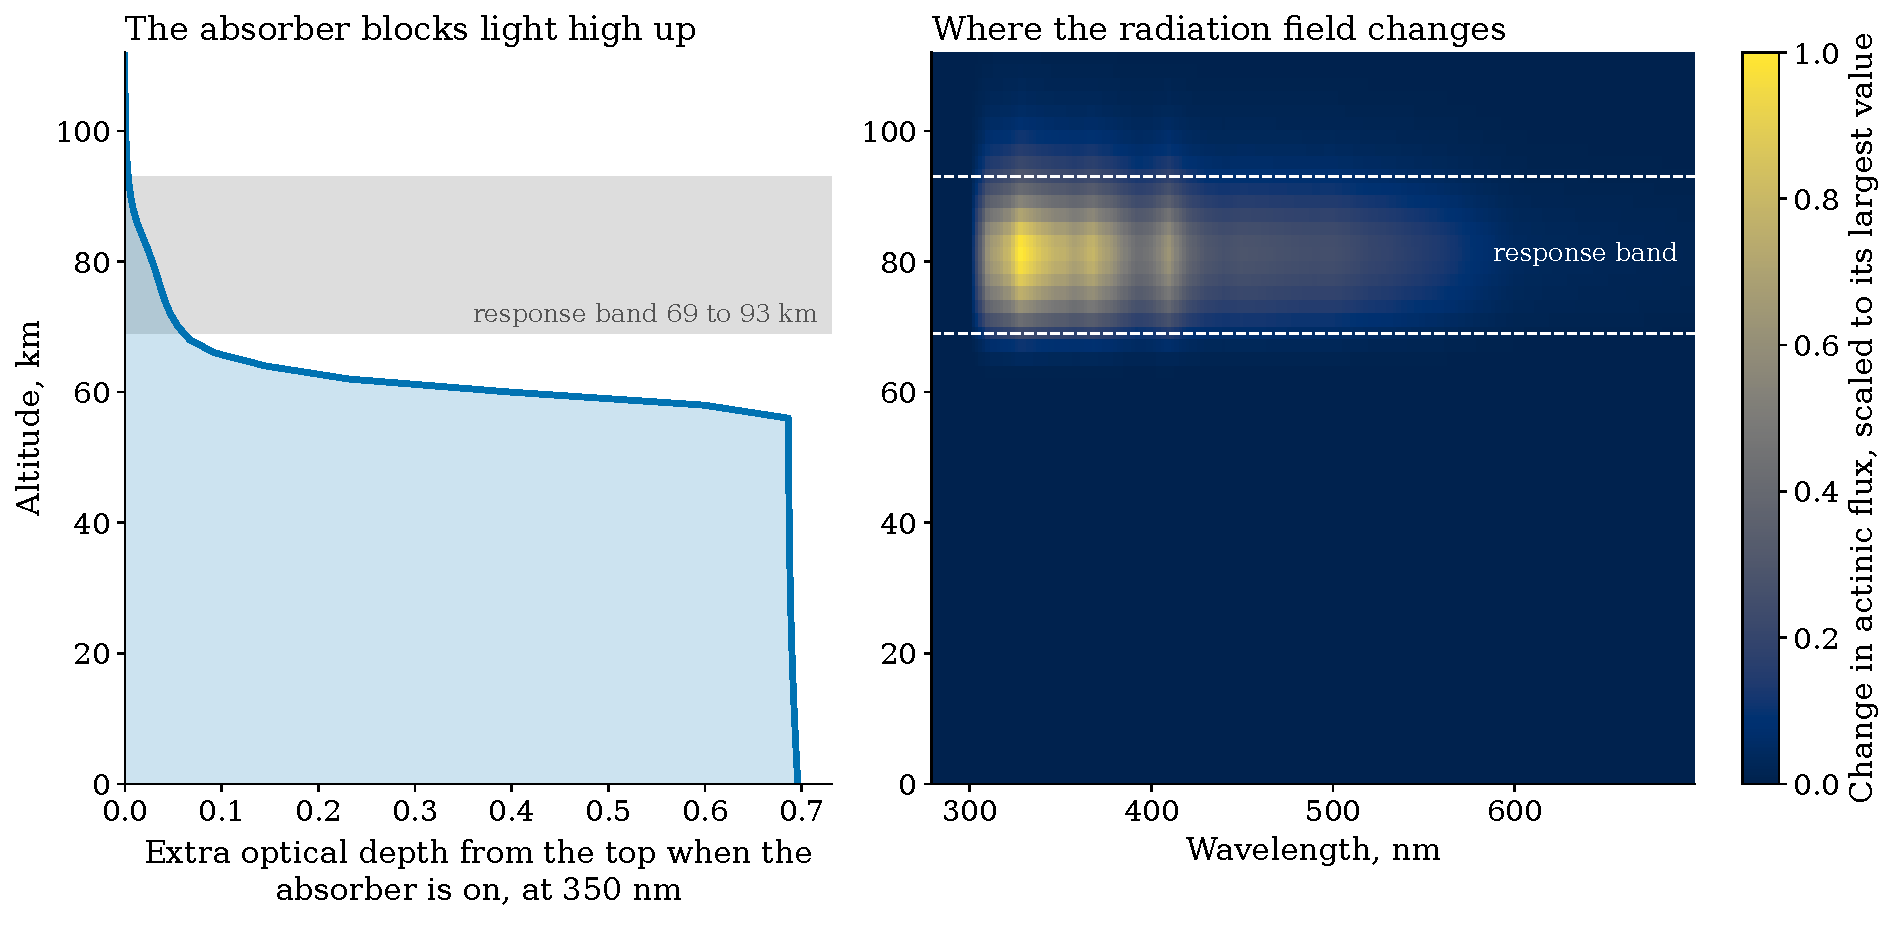
\includegraphics[width=\textwidth]{F05_E01-02_absorber-effect_ch5_s7.pdf}
  \caption[What the absorber does when it is switched on (Experiments~1 and~2)]{What the absorber does when it is switched on (Experiments~1 and~2). Left:
    the extra optical depth, counted from the top of the atmosphere, that the absorber
    adds at 350~nm. Right: the change in actinic flux, scaled to its largest value; it
    sits between 69 and 93~km and mostly between 300 and 420~nm. Sources: committed output of
    Experiments~1 and~2; registry keys \texttt{e6.interval.90.lo} and \texttt{.hi}.}
  \label{fig:F5}
\end{figure}

The composition responds far less. The largest change in the SO\sub{2} mixing ratio is
0.2243\%, and in SO 1.7399\%, both at 71~km (\texttt{e2.SO2.maxrel} and
\texttt{e2.SO.maxrel}). Both are smaller than the reproducibility floor of
Section~\ref{sec:conv-floor}, so they are upper bounds. A strong change in radiation
that leaves the main sulfur species almost unmoved is the pattern that every later
experiment had to explain, and it is why the response was next traced in amount,
wavelength, reaction and altitude.

% ===========================================================================
\section{Experiment 3: is the response proportional?}
\label{sec:e3}

If the response grows in proportion to the amount of absorber, a result found at one
amount holds at any other, and later experiments can compare candidates of different
strength fairly. Besides the control (amplitude 0, run A0) and the nominal run of
Experiment~2 (amplitude 1, run A1), Experiment~3 added two runs, A0.5 at half and A2 at
twice the nominal amplitude.

The test compares the change at half amplitude with half the change at full amplitude,
element by element; a ratio of exactly 1 means proportional. Over the absorber's own
wavelength range, 300 to 698~nm, the median ratio is 1.00002 for optical depth and
1.00208 for actinic flux. Outside that range the two runs differ from the control only
by round-off, thousands of times smaller than the real changes inside it, so a ratio
there carries no information. A second test, on the whole actinic flux field at once,
gives 1.010795 at half amplitude and 0.979304 at twice the amplitude.
Figure~\ref{fig:F6} shows the result.

{\raggedright The keys for these numbers, in order, are
\texttt{e3.\allowbreak lin.\allowbreak tau.\allowbreak inband.\allowbreak median}, \texttt{e3.\allowbreak lin.\allowbreak aflux.\allowbreak inband.\allowbreak median},
\texttt{e3fp.\allowbreak aflux.\allowbreak ratio.\allowbreak A0p5} and \texttt{e3fp.\allowbreak aflux.\allowbreak ratio.\allowbreak A2p0}; the round-off
comparison is \texttt{e3.lin.tau.\allowbreak outband.\allowbreak median\_relsize} against
\texttt{e3.lin.tau.\allowbreak inband.\allowbreak median\_relsize}.\par}

\begin{figure}[tbp]
  \centering
  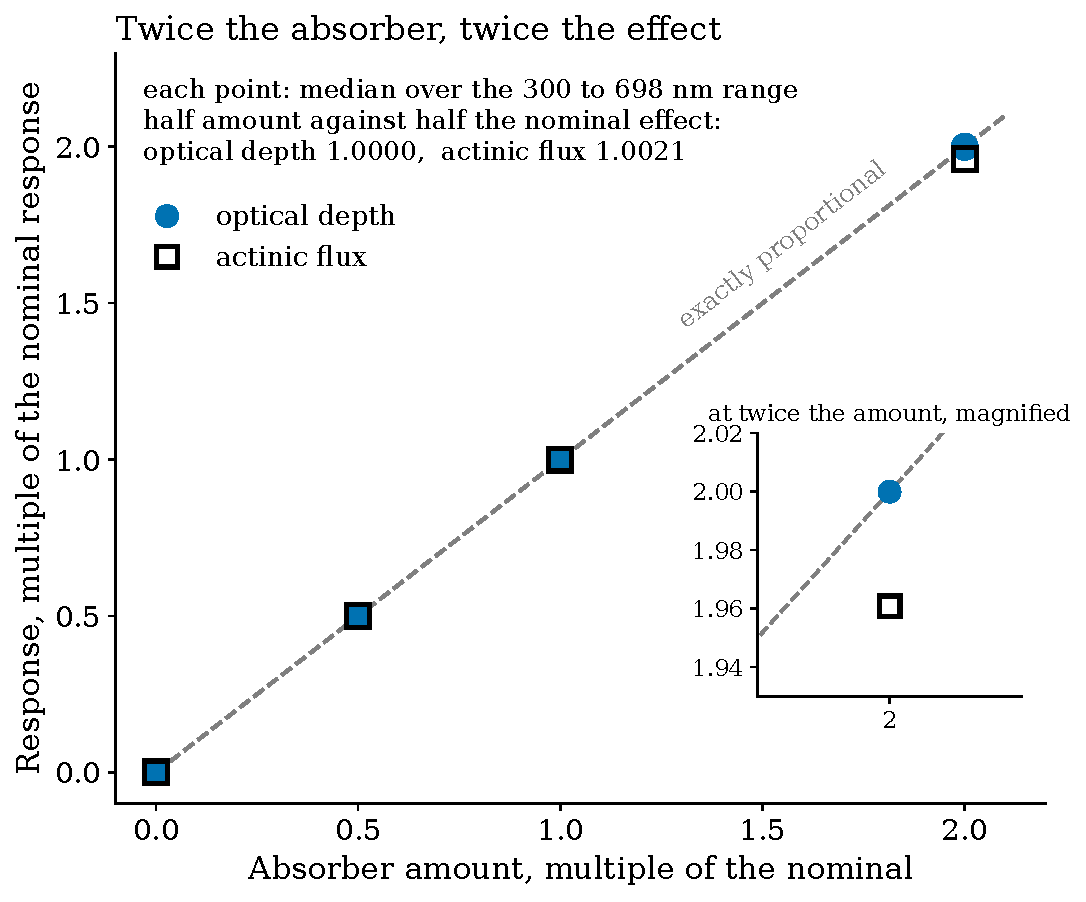
\includegraphics[width=0.6\textwidth]{F06_E03_linear-response_ch5_s8.pdf}
  \caption[The radiative response is proportional to the amount of absorber (Experiment~3)]{The radiative response is proportional to the amount of absorber
    (Experiment~3). Each point is the response at that amount as a multiple of the
    response at the nominal amount. Registry keys \texttt{e3.lin.tau.inband.median} and
    \texttt{e3.lin.aflux.inband.median}.}
  \label{fig:F6}
\end{figure}

The radiative response is therefore proportional to the amount of absorber across a
factor of four. The same test on the sulfur reservoirs gives ratios far from 1 at half
amplitude: for SO\sub{2} it is 1.916 (\texttt{e3fp.L2.A0p5.SO2.ratio}). This
could be read as a sign that the chemistry responds non-proportionally, but that
reading cannot be supported. The SO\sub{2} and SO\sub{3} changes are below the
reproducibility floor: two runs that the radiation cannot tell apart differ in their
reservoirs by about as much (Section~\ref{sec:conv-floor}). SO alone goes above it, at
most 3.316\% at half and 4.379\% at twice the amplitude, inside the band at 71~km
(\texttt{e3fp.A0p5.SO.maxrel\_pct} and \texttt{e3fp.A2.SO.maxrel\_pct}); since the floor
is the smallest the scatter can be (Section~\ref{sec:conv-floor}), that margin is too
narrow to settle the question. The radiative result stands; the chemical one is not
resolved.

% ===========================================================================
\section{Experiment 4: which wavelengths?}
\label{sec:e4}

Experiment~4 asked where in wavelength the response comes from, in two stages.

\textbf{Stage 4A} took the control and the nominal run (A0 and A1) and split each photolysis rate change at
81~km, the middle of the response, into the wavelength windows it came from, using VULCAN's own rule
(Section~\ref{sec:conv-quad}). Different molecules draw on different parts of the
spectrum. S\sub{2}O takes 93.689\% of its change from 300 to 320~nm
(\texttt{e4a.S2O\_1.300\_320.pct}); S\sub{3} takes 49.605\% from 380 to 420~nm; S\sub{4}
takes all of it from beyond 420~nm. SO\sub{2} itself takes none of its change from these
windows, because in the model it is broken apart only by light shorter than 225~nm
(its photolysis cross section, \texttt{cross\_J}, is zero above that). Its photolysis
therefore changes only indirectly, a point Experiment~7 confirms.

Table~\ref{tab:e4a} gives the split for ten sulfur and chlorine photolysis branches,
ordered from the shortest wavelengths to the longest. S\sub{2}O and SO\sub{3} take
nearly all of their change from below 340~nm; S\sub{3}, ClS\sub{2} and SCl take most of
theirs above 380~nm; OSSO, SCl\sub{2} and Cl\sub{2} draw on the whole range. A candidate
that absorbs at some wavelengths therefore affects the photolysis of some molecules and
not others, and which molecules depends on where its absorption lies.

\begin{table}[htbp]
  \centering
  \caption[Where in wavelength each photolysis change comes from (Experiment~4, Stage~4A)]{Where in wavelength the change in each photolysis rate coefficient comes from,
    when the absorber is switched on (Experiment~4, Stage~4A), at 81~km, in per cent of the
    change.
    Ten sulfur and chlorine branches; keys \texttt{e4a.<branch>.<window>.pct}. A row can
    fall short of 100 by the small part from outside these windows.}
  \label{tab:e4a}
  \footnotesize
  \setstretch{1.0}
  \begin{tabular}{lcccccc}
    \toprule
    & \multicolumn{6}{c}{Window (nm)} \\
    \cmidrule(lr){2-7}
    Branch & 300 to 320 & 320 to 340 & 340 to 360 & 360 to 380 & 380 to 420 & 420 to 620 \\
    \midrule
    S\sub{2}O & 93.689 & 6.299 & 0 & 0 & 0 & 0 \\
    SO\sub{3} & 80.754 & 18.795 & 0 & 0 & 0 & 0 \\
    S\sub{2}Cl\sub{2} & 45.016 & 43.215 & 8.574 & 2.872 & 0.319 & 0 \\
    Cl\sub{2} & 17.513 & 40.010 & 25.976 & 11.616 & 4.207 & 0.679 \\
    OSSO (S\sub{2}O\sub{2}) & 13.535 & 25.173 & 21.336 & 19.184 & 14.786 & 5.985 \\
    SCl\sub{2} & 11.427 & 29.895 & 23.971 & 15.863 & 15.974 & 2.869 \\
    S\sub{3} & 0 & 0 & 7.858 & 30.566 & 49.605 & 11.970 \\
    ClS\sub{2} & 0 & 5.785 & 15.369 & 26.717 & 40.776 & 11.353 \\
    SCl & 0 & 0.669 & 5.392 & 10.102 & 31.024 & 52.812 \\
    S\sub{4} & 0 & 0 & 0 & 0 & 0 & 100 \\
    \bottomrule
  \end{tabular}
\end{table}

\textbf{Stage 4B} tested this with six new runs, B1 to B6, each with the absorber spectrum
kept only inside one window: 300 to 320, 320 to 340, 340 to 360, 360 to 380, 380 to 420
and 420 to 698~nm, in that order. Figure~\ref{fig:F7} shows that each run changes the radiation field only where
its absorber absorbs; outside its window the change is too small to see at this scale.
The response is \emph{spectrally local}: what the absorber does at one wavelength does not
depend on what it does at another. This is what makes a test of spectral shape
meaningful in Experiment~12. The six runs also share one response altitude, which
Section~\ref{sec:conv-band} used to show that the response band belongs to the
atmosphere, not to the spectrum.

\begin{figure}[tbp]
  \centering
  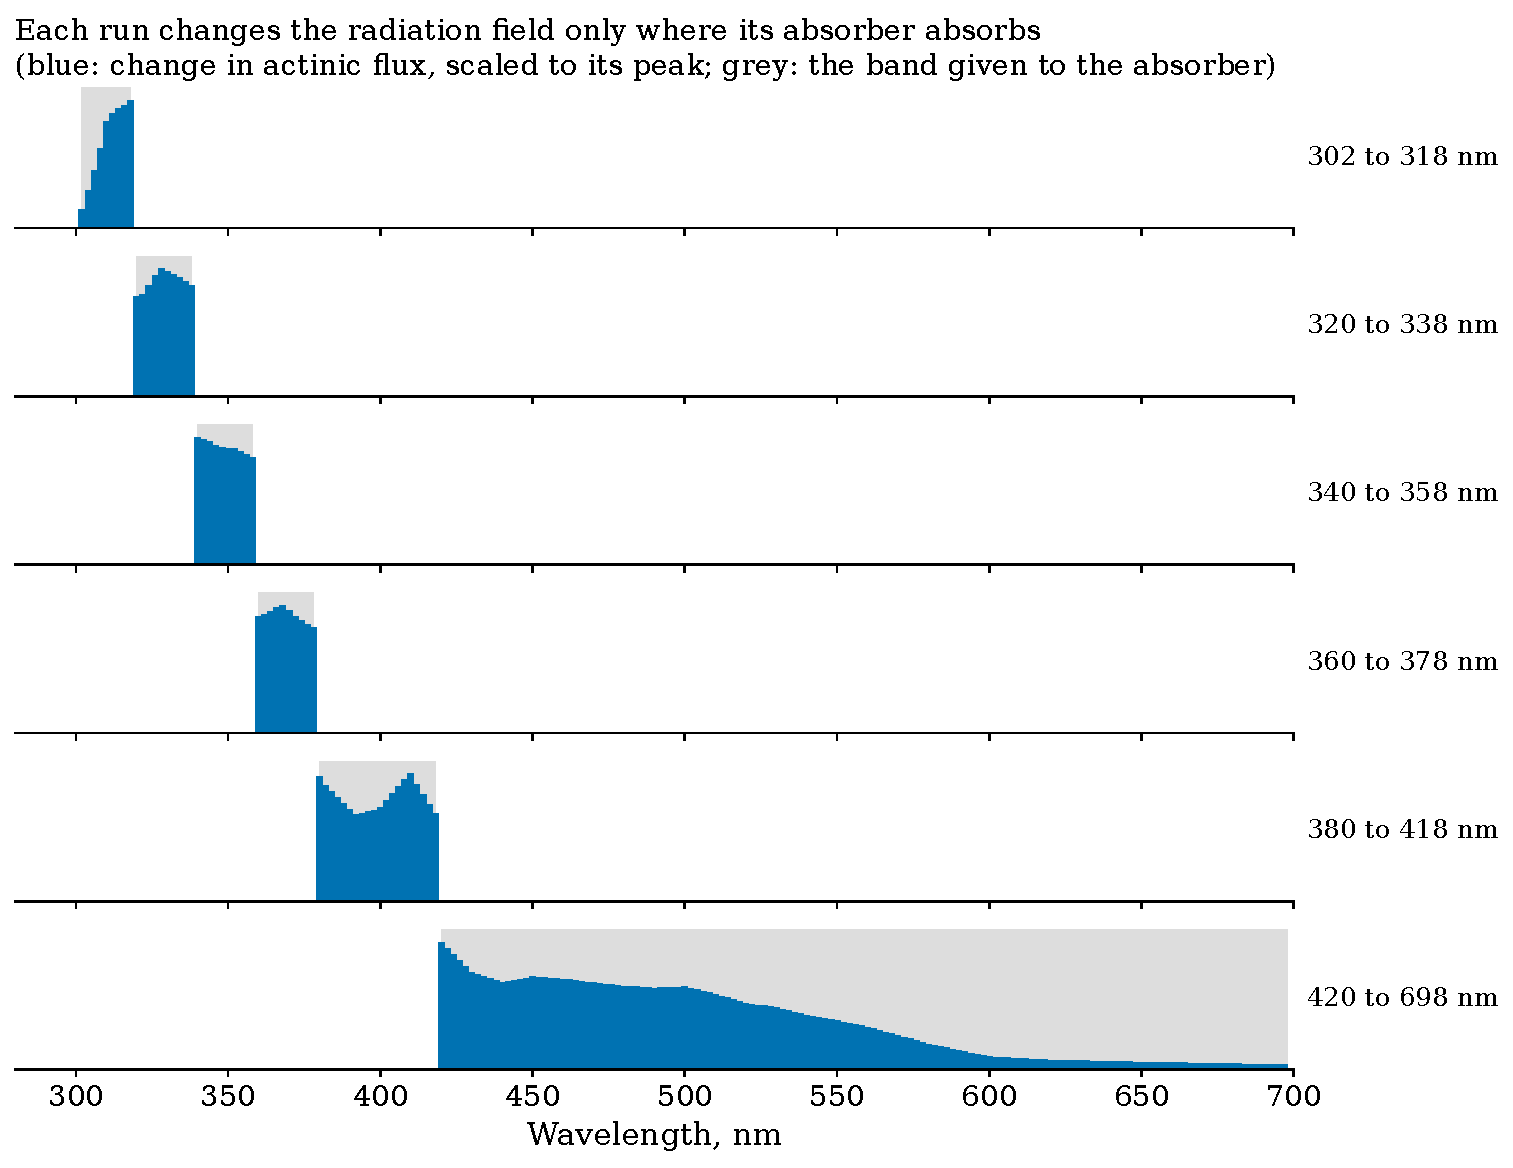
\includegraphics[width=0.82\textwidth]{F07_E04_spectrally-local_ch5_s9.pdf}
  \caption[Each band-limited run changes the radiation field only inside its own window (Experiment~4, Stage 4B)]{Each band-limited run changes the radiation field only inside its own window
    (Experiment~4, Stage 4B). Blue: change in actinic flux, scaled to its peak. Grey: the
    wavelengths given to the absorber in that run. Registry keys
    \texttt{e4b.<run>.support\_lo} and \texttt{.support\_hi}.}
  \label{fig:F7}
\end{figure}

% ===========================================================================
\section{Experiment 5: which reactions?}
\label{sec:e5}

VULCAN writes its chemistry as program code: the rate of change of each species is a
long sum of signed terms, one for each reaction that makes or destroys it. For SO\sub{2}
the sum has 63 terms from 58 distinct reactions (\texttt{e5.SO2.nterms} and
\texttt{.nunique}). Experiment~5 read these terms out of the generated file
\texttt{chem\_funs.py} and evaluated each one in both runs. Adding the terms back
together gives the model's own rate of change exactly, with zero error, for all five
sulfur species examined and in both runs (keys ending \texttt{extraction\_error}). The
attribution is therefore the model's own arithmetic.

\begin{figure}[tbp]
  \centering
  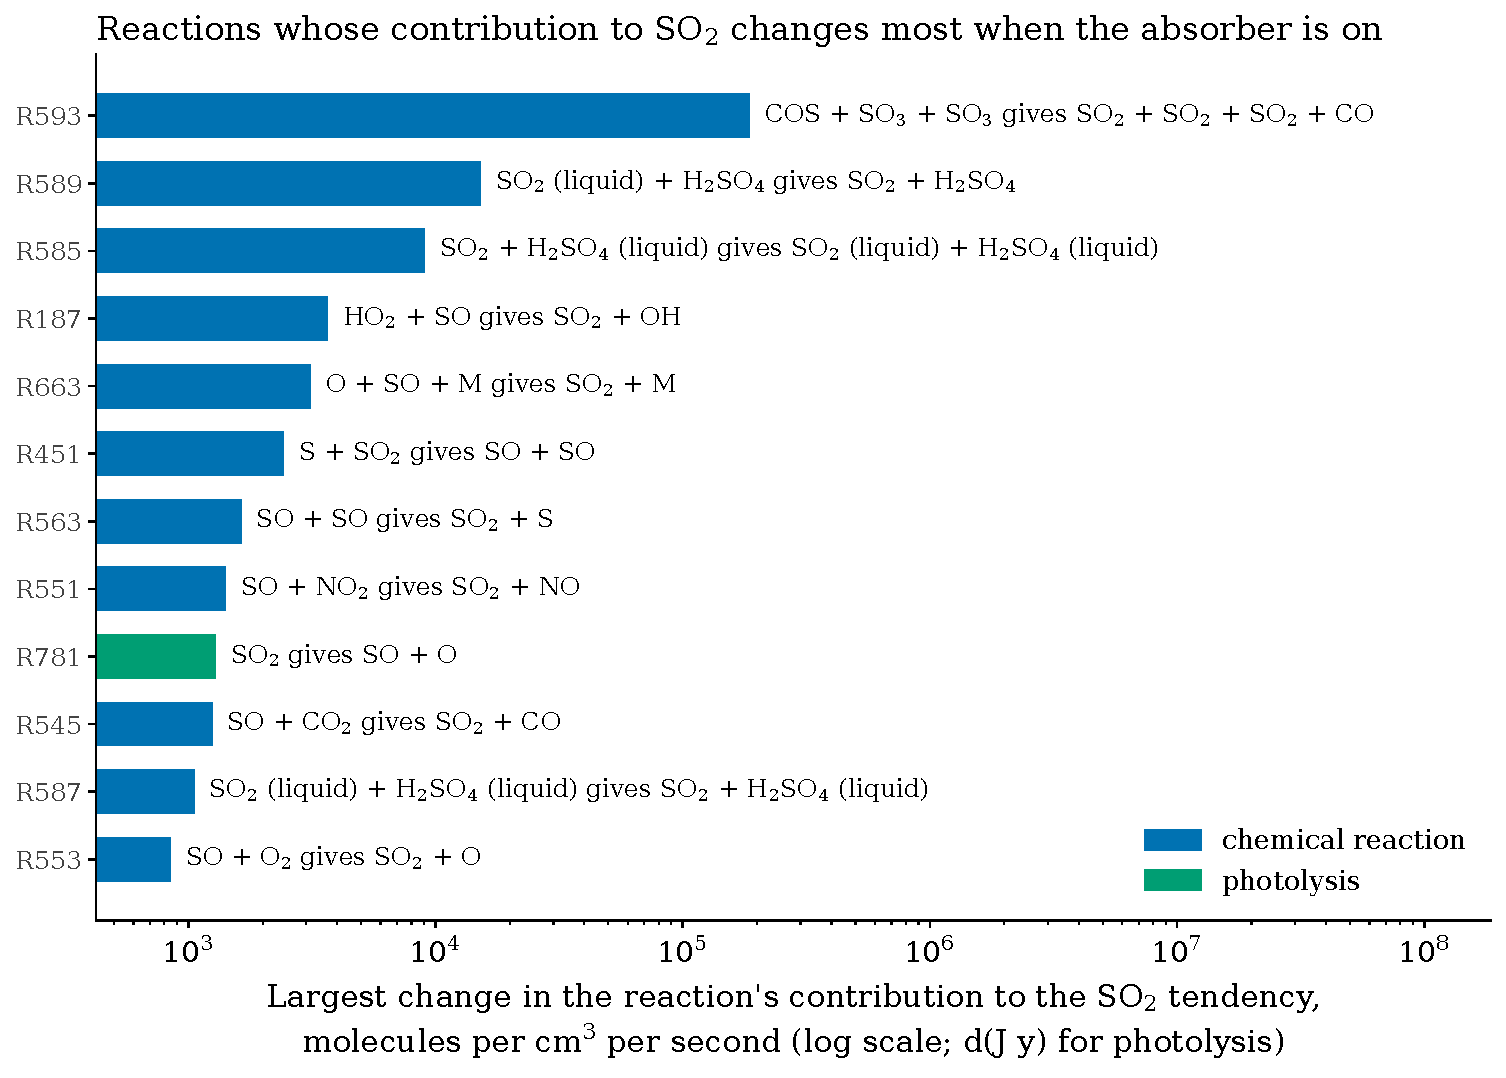
\includegraphics[width=0.86\textwidth]{F08_E05_reaction-pathways_ch5_report.pdf}
  \caption[The reactions whose contribution to SO\sub{2} changes most (Experiment~5)]{The reactions whose contribution to SO\sub{2} changes most when the absorber is
    switched on (Experiment~5), on a logarithmic scale. For the photolysis R781 the
    quantity is the change in rate, $\Delta(Jn)$, written d(J y) on the axis because the
    model calls the number density y. Source: registry keys
    \texttt{e5.SO2.<reaction>.maxdelta}; reaction labels from
    \texttt{thermo/Networks/Nominal.txt}.}
  \label{fig:F8}
\end{figure}

Figure~\ref{fig:F8} ranks the reactions by how much their contribution to SO\sub{2}
changes. The largest change is in R593, COS + SO\sub{3} + SO\sub{3} $\rightarrow$
3\,SO\sub{2} + CO, at $1.8644\times10^{5}$ molecules per cubic centimetre per second at
35~km (\texttt{e5.SO2.R593.maxdelta}). But that reaction runs at $5.7568\times10^{8}$
there (\texttt{e5.SO2.R593.bg\_A0}), so it changes by only 0.032385\%. The oxidation
O + SO + M $\rightarrow$ SO\sub{2} + M (R663) changes by far less in absolute terms but by
1.3809\% of its own rate, at 71~km (\texttt{e5.SO2.R663.frac\_pct}). The absorber reaches
the sulfur chemistry through several coupled reactions, not one, and the largest
absolute change does not mark the most affected reaction. Changes of this size in
reaction rates that depend on abundances also sit below the reproducibility floor, so
the experiment shows \emph{where} the response enters the chemistry more reliably than
\emph{how much}.

% ===========================================================================
\section{Experiment 6: which altitudes?}
\label{sec:e6}

Experiment~6 located the response in altitude. Its radiative part defines the response
band, 69 to 93~km, set out in Section~\ref{sec:conv-band}; Figure~\ref{fig:F9} shows the
profile. The experiment also located the reactions, using the change in rate,
$\Delta(Jn)$ (Section~\ref{sec:conv-J}). The photolysis reactions that the absorber acts
on directly sit in the same band. Of the change in SO\sub{2} photolysis (R781), 99.128\%
falls between 69 and 93~km, with its peak at 71~km (\texttt{e6.R781.pct\_in\_band} and
\texttt{.peak\_z}); for SO\sub{3} photolysis (R787) the share is 99.992\%, peaking at
73~km. Some large changes in other reactions lie much lower: R593 peaks at 35~km and R589
at 53~km, with almost nothing in the band. These are knock-on effects carried through the
chemistry and by mixing, not direct effects of the absorber on sunlight.

\begin{figure}[tbp]
  \centering
  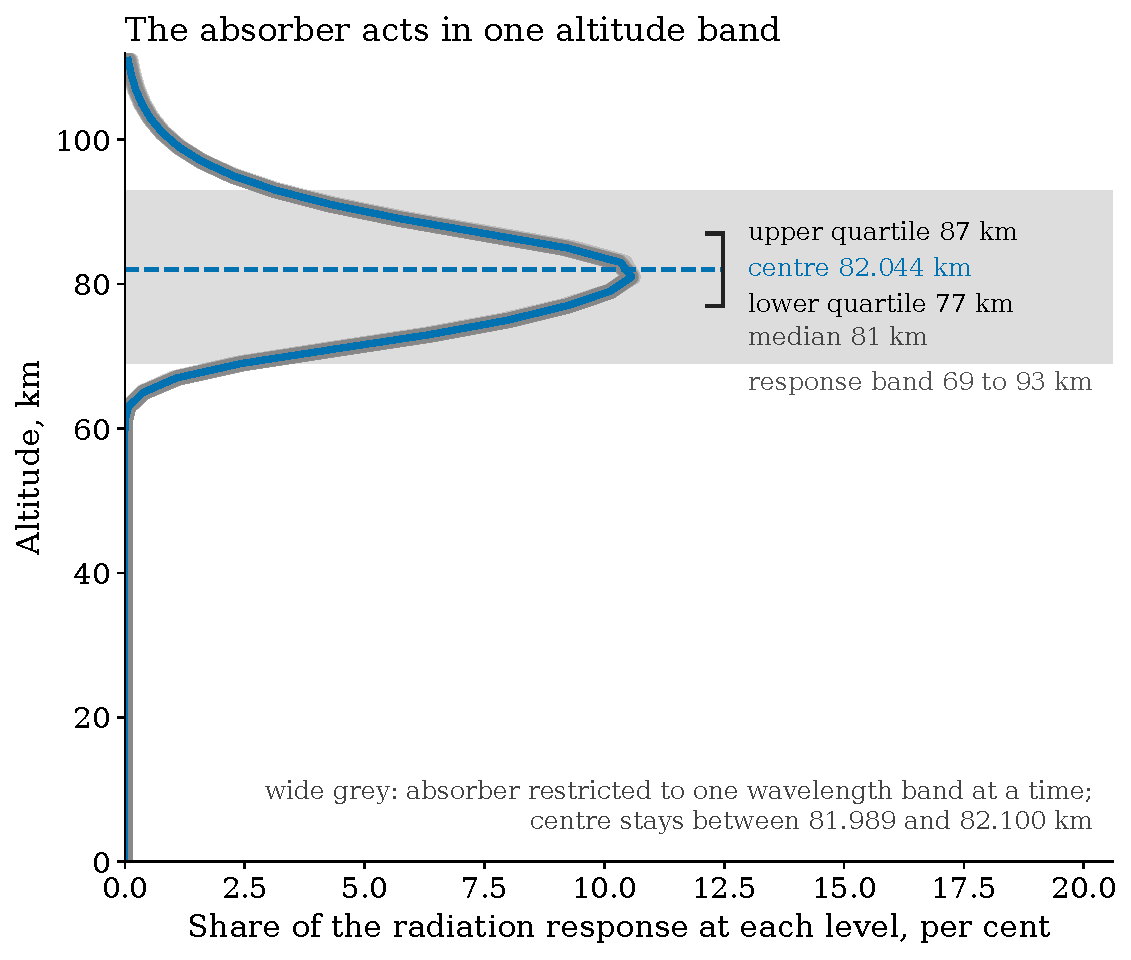
\includegraphics[width=0.6\textwidth]{F09_E06_response-band_ch5_s10.pdf}
  \caption[The share of the radiative response at each altitude (Experiment~6)]{The share of the radiative response at each altitude (Experiment~6). Blue: the
    full absorber. Wide grey lines: the six band-limited runs of Experiment~4. Registry
    keys \texttt{e6.A1.meanz}, \texttt{e6.A1.q25}, \texttt{.q50}, \texttt{.q75},
    \texttt{e6.interval.90.lo} and \texttt{.hi}, \texttt{e6.B5.meanz} and
    \texttt{e6.B6.meanz}.}
  \label{fig:F9}
\end{figure}

% ===========================================================================
\section{Experiment 7: does it matter where the absorber sits?}
\label{sec:e7}

Experiment~7 moved the whole absorber profile up in one run (Experiment~7A) and down in
another (7B), keeping the spectrum, the
amplitude and the total number of particles fixed at $4.0776\times10^{8}$ per square
centimetre (\texttt{e7.nominal.column}). Only the height changed. Its effect is measured
by $\Delta F$ of Equation~\eqref{eq:field}, the size of the change in the whole actinic
flux field as a percentage of the field with the absorber in its usual place.

The nominal profile is centred at 63.419~km (\texttt{e7.nominal.centroid}). Moving it
down by 18~km gives a centre of 45.419~km, a shift of exactly $-18.0000$~km. Moving it
up by 18~km gives 81.263~km, a shift of only $+17.8439$~km (registry key
\texttt{e7.7a.centroid\_shift}), because the top of the profile runs off the top of the
model and the rest is rescaled to keep the total fixed. The two moves are therefore not
mirror images, and the shift must not be written as $\pm 17.844$~km.

\begin{figure}[tbp]
  \centering
  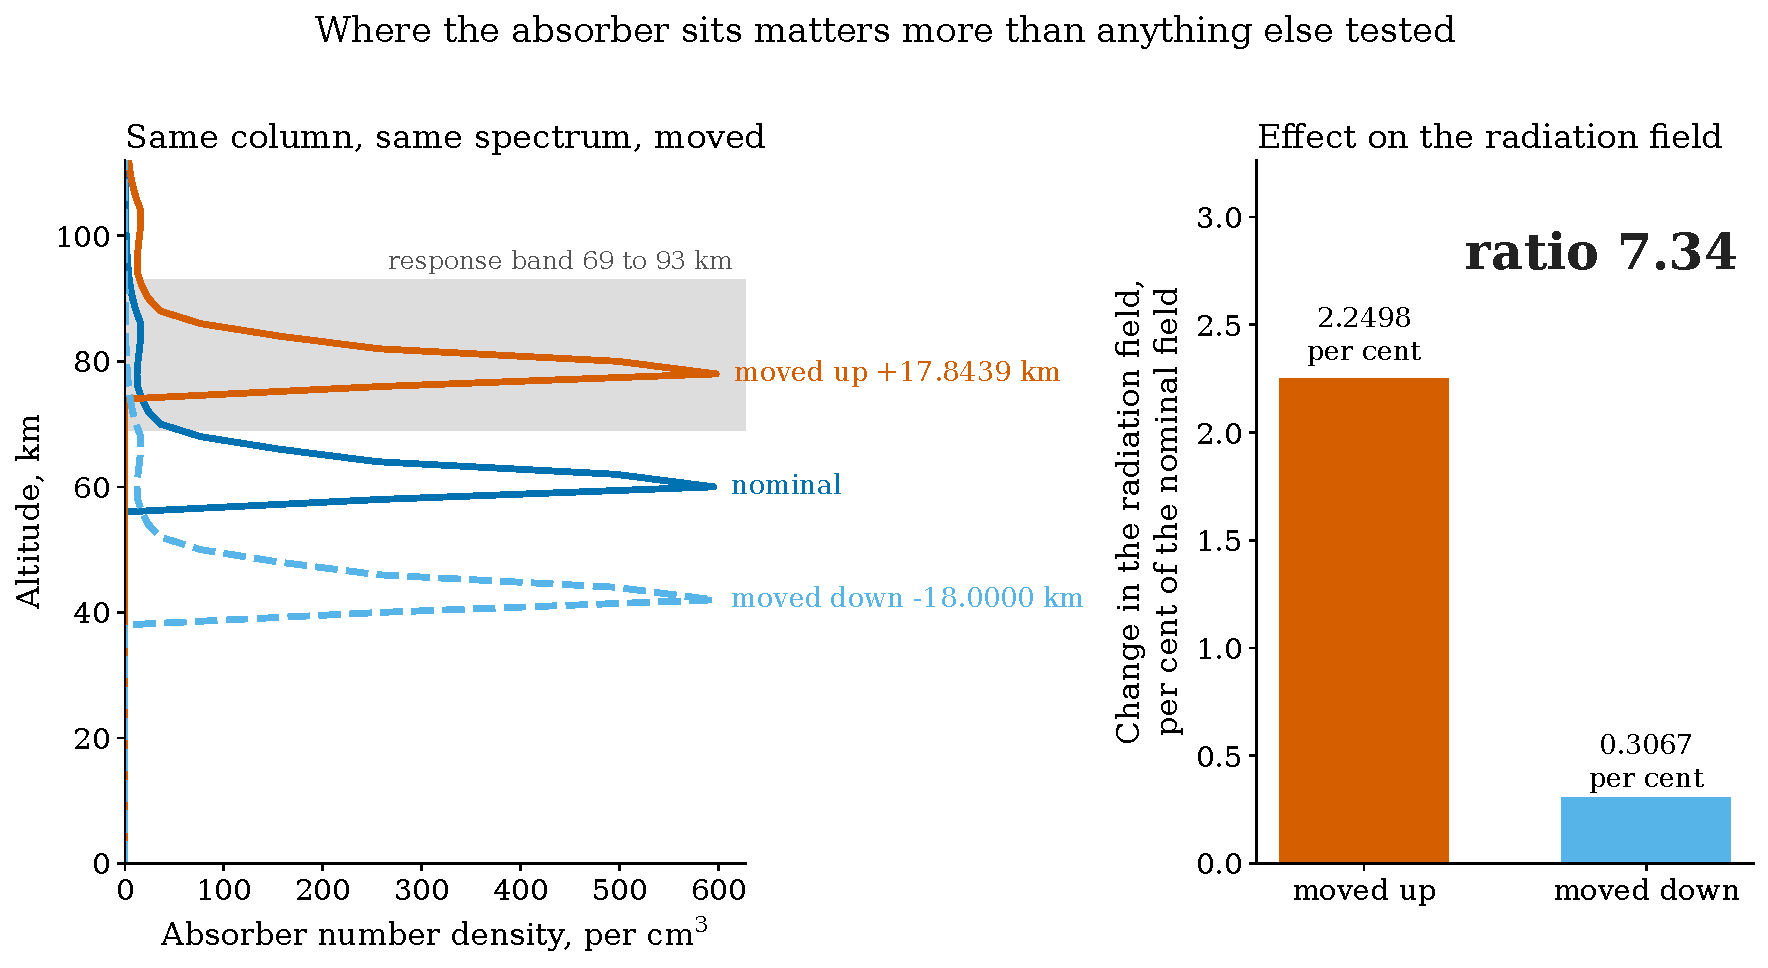
\includegraphics[width=\textwidth]{F10_E07_placement-first-order_ch5_s11.pdf}
  \caption[The same absorber, moved up or down, changes the radiation field by very different amounts (Experiment~7)]{The same absorber, moved up or down, changes the radiation field by very
    different amounts (Experiment~7). Left: the three absorber profiles, with the same
    total. Right: the change in the radiation field as a percentage of the nominal field.
    Registry keys \texttt{e7.7a.centroid\_shift}, \texttt{e7.7b.centroid\_shift},
    \texttt{e7a.L2pct}, \texttt{e7b.L2pct} and \texttt{e7.ratio\_7A\_over\_7B}.}
  \label{fig:F10}
\end{figure}

Figure~\ref{fig:F10} shows the result. Moved up, the absorber changes the radiation field
by 2.2498\% (\texttt{e7a.L2pct}); moved down, by 0.3067\% (\texttt{e7b.L2pct}). The same
amount of the same absorber has 7.34 times more effect when it sits higher
(\texttt{e7.ratio\_7A\_over\_7B}). The responding layer itself barely moves: the response
is centred at 82.435~km in the upward case and 82.355~km in the downward case
(\texttt{e7a.meanalt} and \texttt{e7b.meanalt}), close to the 82.044~km of
Experiment~6. An absorber high up overlaps that layer; the same absorber low down mostly
shades light that has already been weakened.

The chemistry confirms the picture. Three reactions whose rates are set by the local
light, R663, R551 (SO + NO\sub{2} $\rightarrow$ SO\sub{2} + NO) and R665 (O + SO\sub{2} + M
$\rightarrow$ SO\sub{3} + M), change in opposite directions when the absorber moves up
and when it moves down (keys \texttt{e7.7a} and \texttt{e7.7b} ending \texttt{.col}).
Three others, R187, R563 and R781, change in the same direction both ways; why is not yet
known, and it is recorded as an open question, not a result. Table~\ref{tab:e7rx} gives
the numbers: for each reaction, the change in its contribution to the SO\sub{2} budget,
added over the response band with the thickness in centimetres
(Section~\ref{sec:conv-col}). The upward move changes each of them several times more
than the downward move, as it changes the radiation field several times more.

\begin{table}[htbp]
  \centering
  \caption[Change in each reaction's contribution to the SO\sub{2} budget (Experiment~7)]{Change in each reaction's contribution to the SO\sub{2} budget, added over the
    response band, in molecules per square centimetre per second (Experiment~7). A
    positive value means the reaction adds more SO\sub{2} or removes less. Keys
    \texttt{e7.7a.SO2.<reaction>.col} and \texttt{e7.7b.SO2.<reaction>.col}.}
  \label{tab:e7rx}
  \footnotesize
  \setstretch{1.0}
  \begin{tabular}{lllr}
    \toprule
    Reaction & Equation & Moved up (7A) & Moved down (7B) \\
    \midrule
    R663 & O + SO + M $\rightarrow$ SO\sub{2} + M & $-5.6390\times10^{9}$ & $+6.6392\times10^{8}$ \\
    R551 & SO + NO\sub{2} $\rightarrow$ SO\sub{2} + NO & $+6.7343\times10^{9}$ & $-6.7855\times10^{8}$ \\
    R665 & O + SO\sub{2} + M $\rightarrow$ SO\sub{3} + M & $+3.1466\times10^{8}$ & $-6.1425\times10^{7}$ \\
    R187 & HO\sub{2} + SO $\rightarrow$ SO\sub{2} + OH & $-3.8755\times10^{9}$ & $-5.2023\times10^{8}$ \\
    R563 & SO + SO $\rightarrow$ SO\sub{2} + S & $+1.3783\times10^{9}$ & $+3.1740\times10^{8}$ \\
    R781 & SO\sub{2} + $h\nu$ $\rightarrow$ SO + O & $+8.2352\times10^{8}$ & $+2.2860\times10^{8}$ \\
    \bottomrule
  \end{tabular}
\end{table} The upward move changes SO
and SO\sub{3} in the band by 8.404\% and 4.718\% (\texttt{res.e7a.SO.inband} and
\texttt{res.e7a.SO3.inband}), the largest changes in the sulfur
reservoirs in these seven experiments and well above the reproducibility floor; SO
crosses the floor narrowly in Experiment~3 as well, and changes by up to about 3\% in
some Experiment~4B runs (\texttt{e4b.B2.SO.maxrel}). The SO\sub{2} column falls slightly in
both cases, by 0.00048557\% and 0.0016987\% (\texttt{res.e7a.SO2.col} and
\texttt{res.e7b.SO2.col}), so bulk SO\sub{2} does not follow the absorber's height in any
simple way.

% ===========================================================================
\section{What Experiments 1 to 7 establish}
\label{sec:e17-summary}

\begin{itemize}
  \item The absorber term works and the control is exact. Switched on, the absorber
    changes the radiation field strongly and the main sulfur species very little.
  \item The radiative response is proportional to the absorber's amount, and it is
    local in wavelength.
  \item The response lives in one band of altitude, 69 to 93~km, whatever part of the
    spectrum the absorber occupies. It reaches the chemistry through several coupled
    reactions.
  \item Where the absorber sits matters: the same column, moved up instead of down,
    has 7.34 times the effect. Placement is a first-order control, and so a candidate's
    height has to be tested, not assumed. Chapter~6 tests it.
\end{itemize}


% Chapters 6 to 10.
% ===========================================================================
% Chapter 6: Experiments 8 to 14
% Every number below is a registry value, a value printed in a cited paper, or
% an integer count. Registry keys are given in typewriter type.
% ===========================================================================
\chapter{Experiments 8 to 14}
\label{ch:exp814}

Chapter~\ref{ch:exp17} ended with one firm result: the same absorber has 7.34 times more
effect when it sits higher. This chapter compares that with spectral shape
(Experiment~8), lets the model's own chemistry place a candidate (Experiment~9), measures
how far two runs that should agree can differ (Experiment~10), and then tests published
spectra, every species the model can represent, iron minerals and ferric chloride
(Experiments~11 to~14). A change in the radiation field is measured as in
Section~\ref{sec:e7}, as a percentage of the reference field.

% ===========================================================================
\section{Experiment 8: spectral shape at a fixed placement}
\label{sec:e8}

\textbf{Question and design.} If the amount and height of the absorber are held fixed,
how much does the shape of its spectrum matter? Three runs put the spectra of ClS\sub{2}
(Experiment~8A), OSSO, that is S\sub{2}O\sub{2} (8B), and S\sub{3} (8C) in place of the
empirical spectrum, each scaled
so that its absorption added over 300 to 698~nm equals the empirical one, on the
unchanged profile. The optical depth of the absorber above 69~km is then 8.2458 for every
candidate (\texttt{spec\_8A.tau69}) against 8.1928 for the empirical spectrum
(\texttt{spec\_emp.tau69}), only 0.6461\% apart (\texttt{tau.spec\_change\_pct}). The runs
differ only in where along the wavelength axis the absorption sits.

\begin{figure}[tbp]
  \centering
  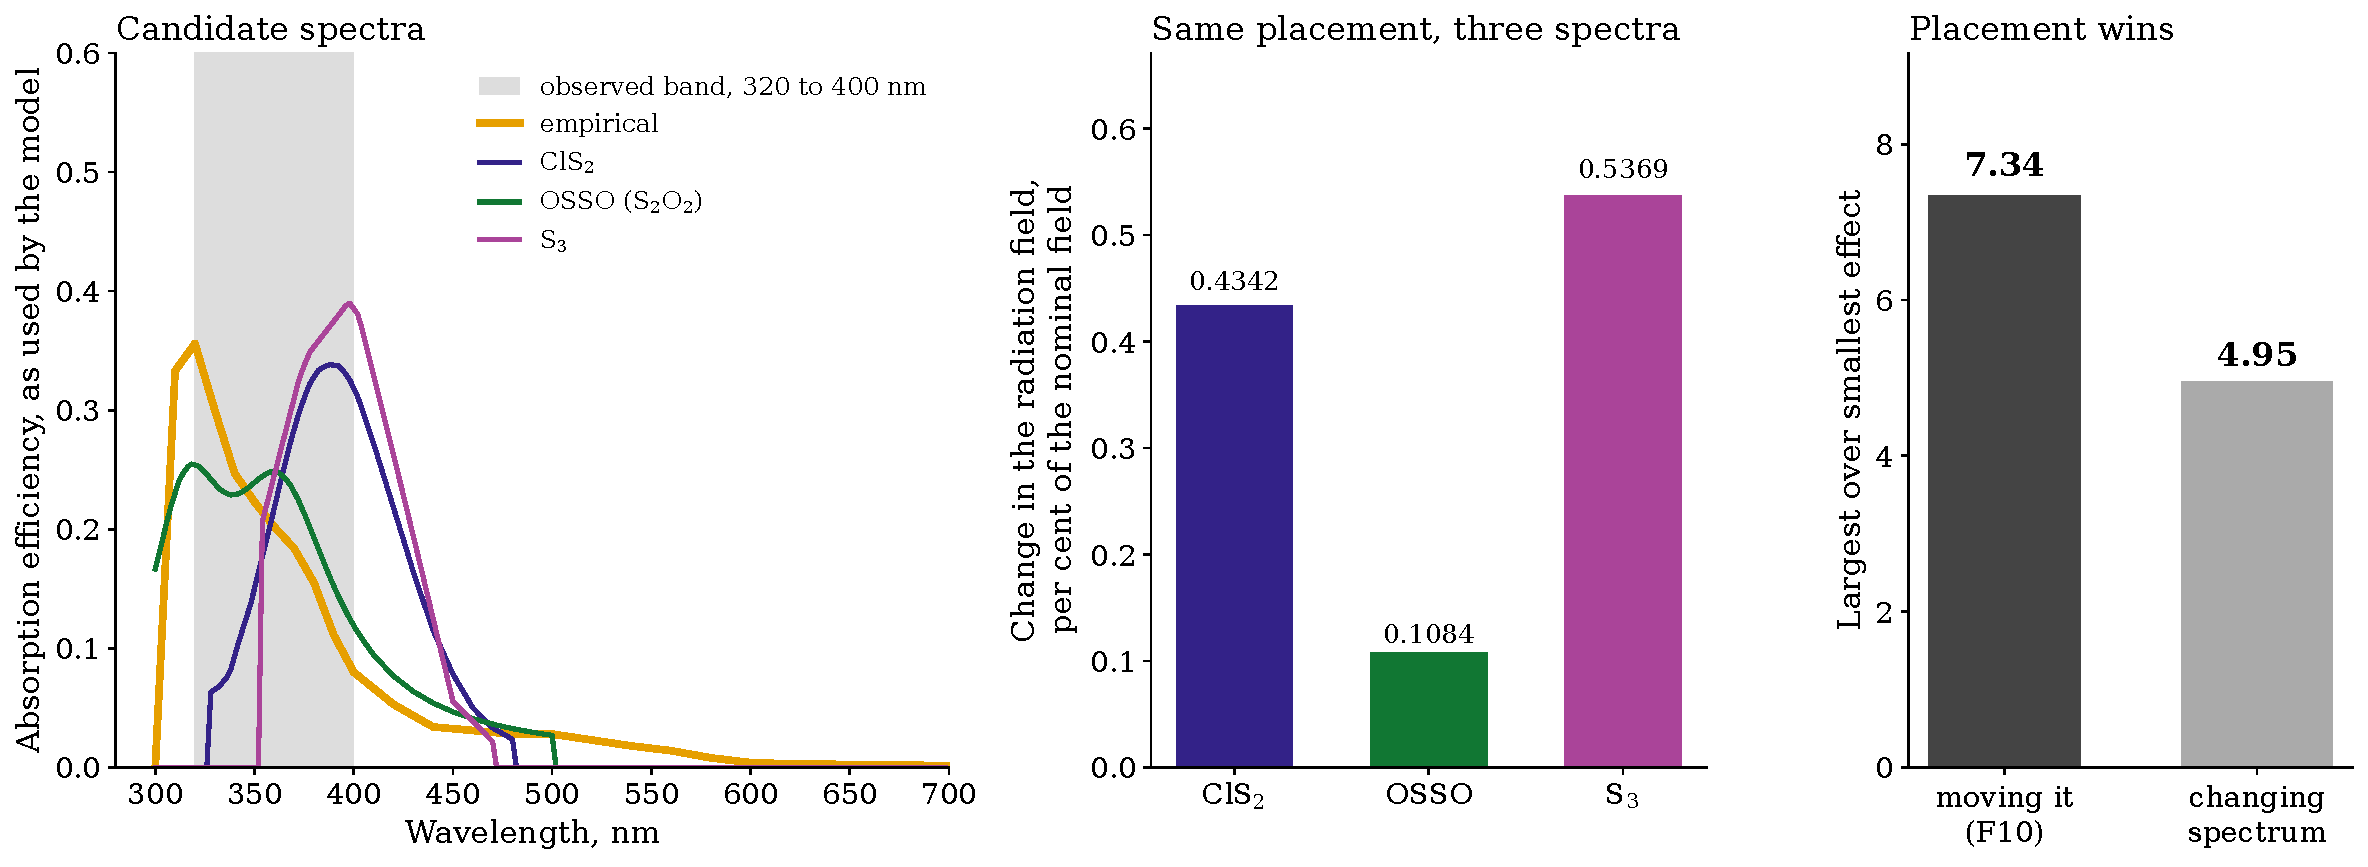
\includegraphics[width=0.92\textwidth]{F11_E08_spectrum-vs-placement_ch6_s12.pdf}
  \caption[Spectral shape against placement (Experiment~8)]{Spectral shape against placement (Experiment~8). Left: the spectra as the model
    uses them. Middle: change in the radiation field for each candidate at the same
    placement. Right: largest over smallest effect, for moving the absorber
    (Experiment~7) and for changing its spectrum. Keys \texttt{e8a.L2pct},
    \texttt{e8b.L2pct}, \texttt{e8c.L2pct}, \texttt{e7a.L2pct} and \texttt{e7b.L2pct}.}
  \label{fig:F11}
\end{figure}

\textbf{Result.} The radiation field changes by 0.4342\% for ClS\sub{2}, 0.1084\% for
OSSO and 0.5369\% for S\sub{3} (\texttt{e8a.L2pct}, \texttt{e8b.L2pct},
\texttt{e8c.L2pct}; Figure~\ref{fig:F11}). The largest is 4.95 times the smallest, so
spectral shape is a real, independent control. But moving the absorber changed the effect
7.34-fold, and the largest spectral effect is well below the 2.2498\% of the upward move.
\emph{Placement matters more than spectral shape, and spectral shape is not negligible.}
This comparison is the quantitative core of Phase~1. One caution: the responses are in the
reverse order of each spectrum's correlation with the empirical one, 0.9394 for OSSO,
0.3419 for ClS\sub{2} and 0.2253 for S\sub{3} (\texttt{corr.8B}, \texttt{corr.8A},
\texttt{corr.8C}). Since the empirical spectrum was fitted to the observed brightness of
Venus, the ranking measures resemblance to that fit, not correctness.

\textbf{The amount check.} A script that only reads the saved baseline divided the
required optical depth $\tau_{\mathrm{req}}$ (Section~\ref{sec:taureq}) by the optical
depth that each of twelve sulfur and chlorine species gives with its column above 58~km,
at the wavelength where its absorption peaks within 300 to 620~nm. The result, the
\emph{shortfall factor},
is how many times too little of the species there is. ClS\sub{2} comes closest, short by
121.914 at 388~nm (\texttt{scr.ClS2.short}), about two orders of magnitude; next is
S\sub{2}O at 6070, and the rest are short by $4.4\times10^{4}$ (\texttt{scr.S2.short}) to
$4.2\times10^{8}$ (\texttt{scr.SCl.short}). OSSO is short by $4.2\times10^{6}$
(\texttt{scr.S2O2.short}). Egan et al.\ found OSSO about three orders of magnitude too low
by a different route~\cite{egan2025osso}. The two agree in direction and differ in size
because they measure against different things, and theirs uses SO\sub{2} above the clouds
kept deliberately high to give OSSO every chance~\cite{egan2025osso}. OSSO is the only
candidate with an independent published verdict, so this agreement is the main outside
check on the screen's arithmetic. ClS\sub{2}, the one species close in amount, went
forward to Experiment~9. Table~\ref{tab:scr} lists all twelve.

\begin{table}[htbp]
  \centering
  \caption[The amount check (Experiment~8)]{The amount check of Experiment~8: each species' column above 58~km, at the
    wavelength where its absorption peaks within 300 to 620~nm, against the required
    optical depth. Keys
    \texttt{scr.<species>.lam} and \texttt{scr.<species>.short}.}
  \label{tab:scr}
  \footnotesize
  \setstretch{1.0}
  \begin{tabular}{lcc}
    \toprule
    Species & Peak wavelength (nm) & Shortfall factor \\
    \midrule
    ClS\sub{2} & 388 & $1.219\times10^{2}$ \\
    S\sub{2}O & 300 & $6.070\times10^{3}$ \\
    S\sub{2} & 300 & $4.415\times10^{4}$ \\
    S\sub{3} & 398 & $7.486\times10^{4}$ \\
    S\sub{4} & 500 & $9.962\times10^{4}$ \\
    ClO & 300 & $6.754\times10^{5}$ \\
    SCl\sub{2} & 338 & $8.049\times10^{5}$ \\
    S\sub{2}Cl\sub{2} & 300 & $1.092\times10^{6}$ \\
    Cl\sub{2} & 328 & $1.604\times10^{6}$ \\
    OSSO & 318 & $4.207\times10^{6}$ \\
    SO\sub{3} & 300 & $8.626\times10^{6}$ \\
    SCl & 470 & $4.205\times10^{8}$ \\
    \bottomrule
  \end{tabular}
\end{table}

% ===========================================================================
\section{Experiment 9: letting the chemistry place the candidate}
\label{sec:e9}

\textbf{Question and design.} Experiments~7 and~8 used the empirical profile, a height
chosen by the modeller. What happens when a candidate sits where the model's own
chemistry puts it? The ClS\sub{2} spectrum was kept, and the absorber profile was given
the shape of the model's own steady-state ClS\sub{2} profile, rescaled so that the sum of
the absorber over all levels stayed the same. The expected outcome was written down
before the run: if the absorber left the response band, the run should reproduce the
difference between the runs with and without the absorber (Section~\ref{sec:e6}), with
the opposite sign.

\begin{figure}[tbp]
  \centering
  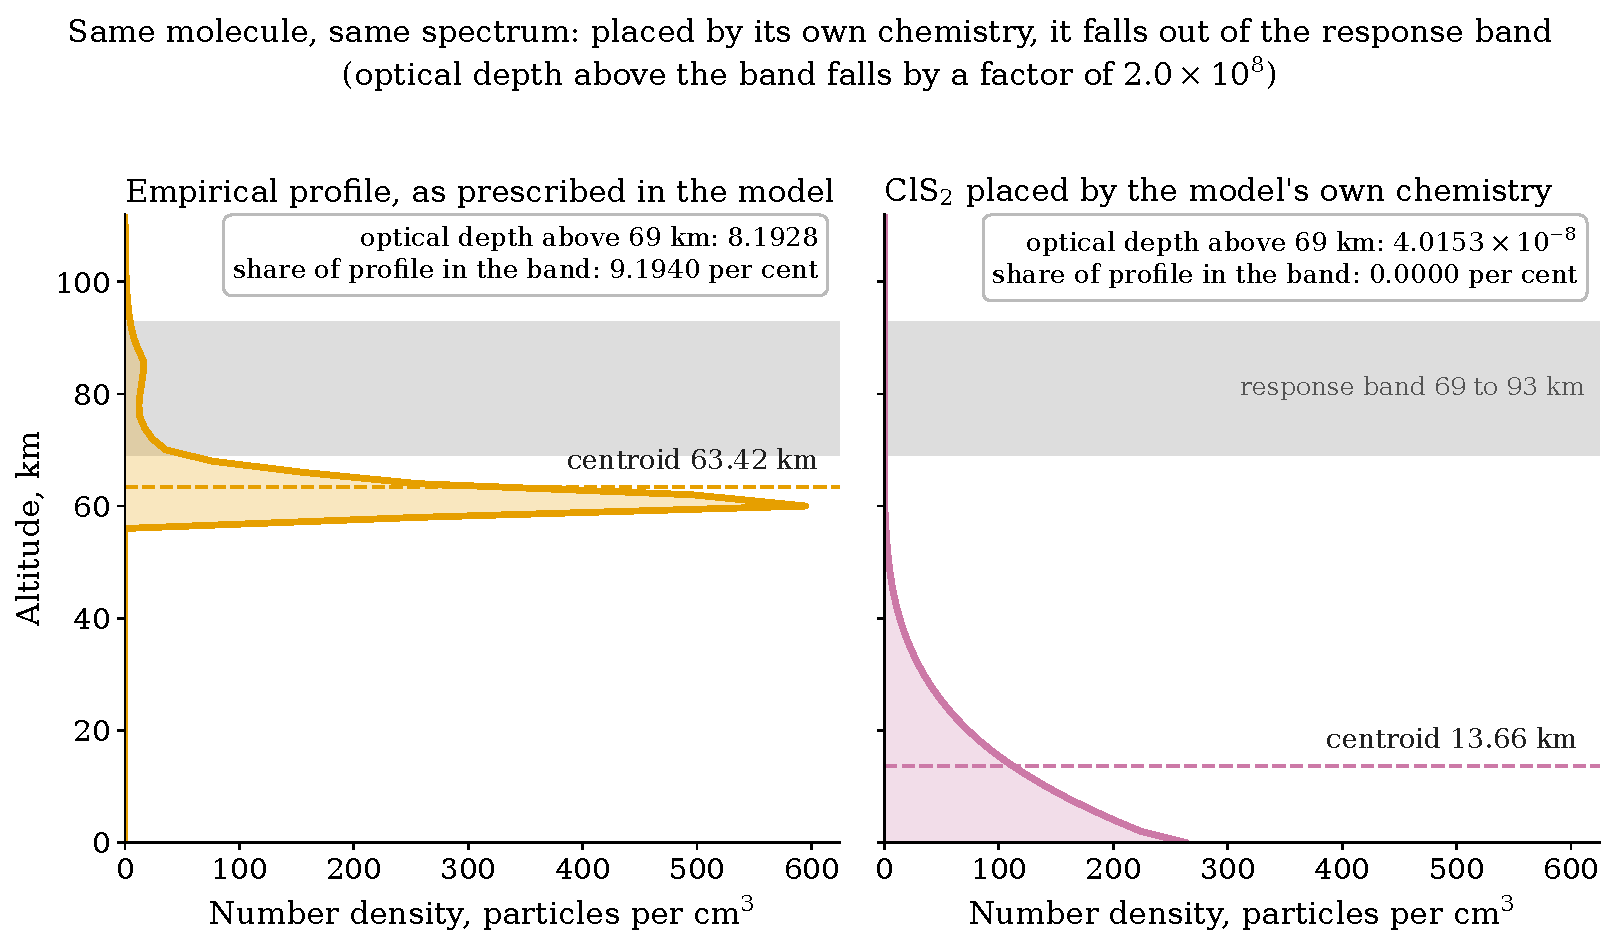
\includegraphics[width=0.8\textwidth]{F12_E09_ClS2-self-placement_ch6_s13.pdf}
  \caption[The same molecule and spectrum, placed two ways (Experiment~9)]{The same molecule and spectrum, placed two ways (Experiment~9). Left: the
    empirical profile. Right: the profile the model's own chemistry gives ClS\sub{2}. The
    grey band is the response band. Keys \texttt{pnom.centroid}, \texttt{p9.centroid},
    \texttt{spec\_emp.tau69}, \texttt{spec\_9.tau69}, \texttt{pnom.inband},
    \texttt{p9.inband} and \texttt{tau.reduction}.}
  \label{fig:F12}
\end{figure}

\textbf{Where the chemistry puts it.} The empirical absorber is a layer at the cloud top,
centred at 63.419~km (\texttt{pnom.centroid}), with 9.1940\% of its column inside the
response band (\texttt{pnom.inband}). The model's ClS\sub{2} is centred at 13.656~km
(\texttt{p9.centroid}), 51.521~km lower (\texttt{e9.centroid\_shift}), with 91.80\% of it
below 30~km (\texttt{p9.below30}) and 0.0000\% inside the band (\texttt{p9.inband};
Figure~\ref{fig:F12}). The registry shows where the chemistry puts it, not why; how fast
ClS\sub{2} is made and destroyed at each height is the quantity Phase~2 measures first
(Chapter~\ref{ch:phase2}, WP5). The optical depth above 69~km
falls from 8.1928 to $4.0153\times10^{-8}$ (\texttt{spec\_9.tau69}), a factor of
$2.0\times10^{8}$ (\texttt{tau.reduction}). Keeping the level sum fixed left the column
(Section~\ref{sec:conv-col}) 12.88\% lower (\texttt{p9.col\_deficit\_pct}), because the
new profile puts that share of its level sum in the model's lowest layer, which is only
2~cm thick; beside a factor of $2.0\times10^{8}$ this cannot matter.

\textbf{Result.} The prediction held. The peak change in actinic flux has the size and
place of the no-absorber control, at 81~km and 328~nm, with the opposite sign. Added cell
by cell, the two change fields leave 0.001487\% of the control
(\texttt{id.l2\_ratio\_pct}), and over the 3425 cells carrying more than 1\% of the peak
their ratio has mean 0.99994 and standard deviation $9.4\times10^{-5}$
(\texttt{id.ratio\_mean}, \texttt{id.ratio\_sd}).

\emph{This is the central result of Phase~1.} Placed where the model's own chemistry puts
it, ClS\sub{2} is radiatively the same as no absorber at all in the band where the
absorber acts. It is in the calculation at full strength, with a spectrum in the right
range, but in the wrong place. A candidate can come close in amount and have a suitable
spectrum and still be invisible, because the chemistry places it below the altitudes where
the radiation responds. This failure is separate from its shortfall in amount.

The two photolysis conventions of Section~\ref{sec:conv-J} give different pictures here,
and both are correct. Nearly every rate coefficient rises a little, the largest
$\Delta J$ being 3.168\% for S\sub{2}O\sub{2} at 81~km (\texttt{dJ.e9.S2O2}); those of
SO\sub{2} and SO fall very slightly (\texttt{dJ.e9.SO2}, \texttt{dJ.e9.SO}). But the rate
$\Delta(Jn)$ of S\sub{2}Cl\sub{2} and SCl\sub{2} photolysis falls by 21.751\% and
19.630\% at 69~km (\texttt{dJy.e9.S2Cl2}, \texttt{dJy.e9.SCl2}). Since the coefficients
rise, these falls come from smaller amounts of the two molecules, and those amounts are
abundances, which the floor of Section~\ref{sec:conv-floor} limits; no cause is claimed
for them. The largest change among the sulfur reservoirs in the band, SO by 0.7384\%
(\texttt{res.e9.SO.inband}), is below that floor, so no abundance result is claimed.

% ===========================================================================
\section{Experiment 10: a replicate, two floors and a retraction}
\label{sec:e10}

Experiment~10 put the S\sub{3} spectrum on the same ClS\sub{2} profile, to test whether a
pattern seen in Experiment~9 held for a third combination. The test was void: both
spectra lie wholly inside the range used for scaling and were scaled to the same total on
the same profile, so the optical depth above 69~km is identical to every digit kept
(\texttt{tau.9\_minus\_10} is zero), and the difference between the two actinic flux
fields is only 0.0017\% of the change that Experiment~9 makes
(\texttt{e10.fielddiff\_pct}; Section~\ref{sec:conv-field}). Experiment~10 is a numerical replicate of
Experiment~9, and that accident gave three results.

\begin{figure}[tbp]
  \centering
  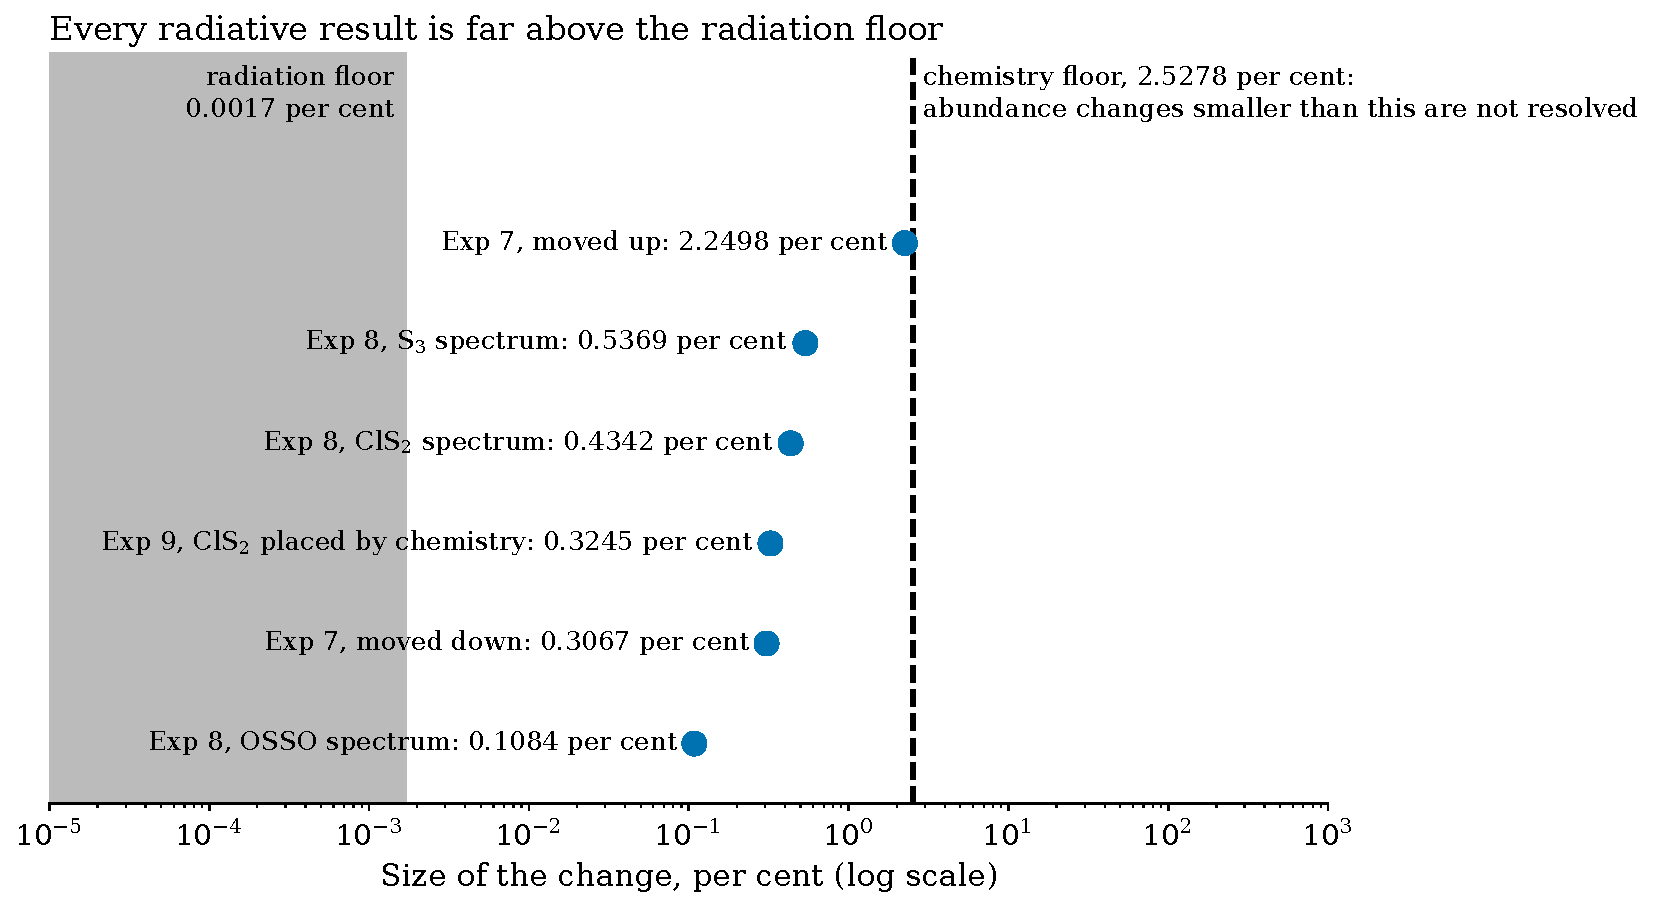
\includegraphics[width=0.8\textwidth]{F13_E10_noise-floors_ch6_backup.pdf}
  \caption[The two floors (Experiments~9 and~10)]{The two floors (Experiments~9 and~10). Every radiative result lies far above
    the radiation floor of 0.0017\% (\texttt{e10.fielddiff\_pct}), which is a share of the
    change Experiment~9 makes and so smaller still as a share of the field; the chemistry
    floor of 2.5278\% (\texttt{res.e10.SO.inband}) applies to abundances only.}
  \label{fig:F13}
\end{figure}

\textbf{Two floors, not one.} Since the radiation fields agree, any difference in the
chemistry is numerical. SO in the band differs from the baseline by 0.7384\% in one run
and 2.5278\% in the other (\texttt{res.e10.SO.inband}): this is the chemistry floor of
Section~\ref{sec:conv-floor}. Figure~\ref{fig:F13} sets it beside the radiation floor of
0.0017\%. The two numbers are not on the same footing. Every radiative result, from
0.1084\% for OSSO to 2.2498\% for the upward move, is a share of the field
(Equation~\eqref{eq:field}); the radiation floor is a share of the change Experiment~9
makes, and that change is itself only 0.3245\% of the field (\texttt{e9.L2pct}). Two runs
that should agree therefore differ by far less than any result, so every radiative
comparison stands; the chemistry floor limits only claims about abundances. Only two abundance changes in the
project exceed it clearly: those of SO and SO\sub{3} when the absorber is moved up
(Section~\ref{sec:e7}); SO also crosses it narrowly in Experiments~3 and~4B.

\textbf{Spectral shape matters only where the absorber overlaps the responding layer.}
On the empirical profile, S\sub{3} gives 1.2365 times the effect of ClS\sub{2}; on the
ClS\sub{2} profile the same ratio is 1.000003. Out of the band, the spectrum no longer
matters (keys \texttt{twoby2.nominal\_ratio} and \texttt{twoby2.cls2\_ratio}).

\textbf{A retraction.} In Experiment~9 the change in each of nine photolysis rate
coefficients was the change in Experiment~7B times one constant, 1.0474 with standard
deviation 0.00056 (\texttt{chr.mean}, \texttt{chr.sd}); the nine ratios are ClS\sub{2} 1.0473, H\sub{2}SO\sub{4} 1.0466, S\sub{2}Cl\sub{2} 1.0482, S\sub{2}O 1.0480, OSSO 1.0477, S\sub{3} 1.0472, S\sub{4} 1.0466, SCl 1.0469, SCl\sub{2} 1.0477 (keys \texttt{chr.<species>}). This had been read as a
``fingerprint'' of absorbers below the cloud top. It is not: the ratio of the actinic flux
changes themselves at 81~km, the peak response height, added over all wavelengths, is
1.0473 (\texttt{chr.flux\_ratio}). The constant is linear response; when two small disturbances
change the light in the same place, every photolysis rate follows the light. For
Experiment~7A, where the optical depth above 69~km is 10.1975 times the nominal
(\texttt{tau.7A\_over\_A1}), the ratios for eight of the species scatter widely (mean $-14.12$, spread 12.43;
\texttt{chr8\_7a\_7b.mean} and \texttt{.spread}),
which locates the edge of the linear regime. The fingerprint reading is withdrawn in
commit \texttt{5a7e2ac}.

% ===========================================================================
\section{Experiment 11: computed cross sections of two isomers}
\label{sec:e11}

\textbf{Question and design.} Trabelsi and Francisco computed the cross sections of two
chlorine and sulfur isomers, ClSSCl and SSCl\sub{2}, and offer them as model
inputs~\cite{trabelsi2026}; the model tracks only one lumped species, S\sub{2}Cl\sub{2}.
The computed data, obtained from the authors and checked against their published figure,
were run as absorber spectra under the rules of Experiment~8, SSCl\sub{2} in
Experiment~11A and ClSSCl in 11B.

\begin{figure}[tbp]
  \centering
  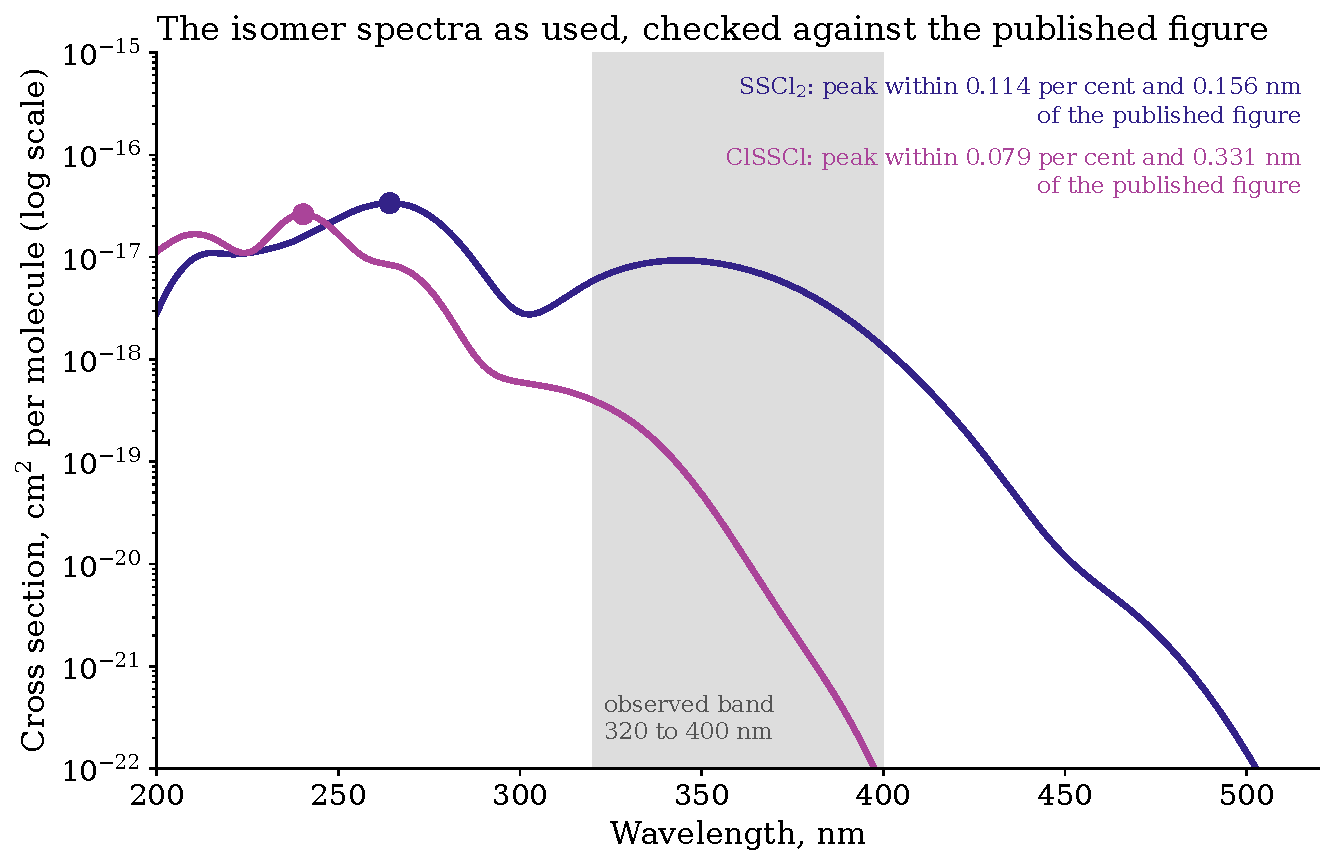
\includegraphics[width=0.66\textwidth]{F14_E11_published-cross-sections_ch6_report.pdf}
  \caption[The isomer cross sections as used, checked against the published figure (Experiment~11)]{The isomer cross sections as used, checked against the published figure
    (Experiment~11). Keys \texttt{iso.SSCl2.val\_pct}, \texttt{iso.SSCl2.val\_nm},
    \texttt{iso.ClSSCl.val\_pct} and \texttt{iso.ClSSCl.val\_nm}.}
  \label{fig:F14}
\end{figure}

\textbf{Result.} Each peak matches the published figure to 0.114\% in height and
0.156~nm in position for SSCl\sub{2}, and 0.079\% and 0.331~nm for ClSSCl
(Figure~\ref{fig:F14}). SSCl\sub{2} puts 85.49\% of its absorption between 320 and
400~nm, more than any other spectrum tested and more than the empirical 61.58\%; its
correlation with the empirical spectrum, 0.88983, is second to OSSO's (keys
\texttt{share320400.11A}, \texttt{share320400.emp} and \texttt{corr.11A}). It is therefore the best
match by share but only the second by correlation. On the empirical profile
the field changes by 0.19465\% for SSCl\sub{2} and 0.30144\% for ClSSCl
(\texttt{e11a.L2pct}, \texttt{e11b.L2pct}). Across all five spectra the responses fall in
exactly the reverse order of their correlations (rank correlation $-1$,
\texttt{five.spearman}), with the caution of Experiment~8.

Neither isomer can be made in the amount needed: at its absorption peak within 300 to
620~nm SSCl\sub{2} is short
by $4.266\times10^{5}$ and ClSSCl by $6.668\times10^{6}$ (\texttt{iso.SSCl2.short},
\texttt{iso.ClSSCl.short}). ClSSCl absorbs most strongly near 240~nm, below the start of
the absorber's grid at 300~nm, so the model sees only its tail, scaled up to a peak
efficiency of 0.9467 against the empirical 0.356 (\texttt{spec\_11B.peakQ}); its response
describes that tail, not the molecule. Within the literature reviewed in
Chapter~\ref{ch:lit}, no earlier study has run computed chlorine and sulfur cross sections
in a Venus photochemistry model; this is the extent of the review, not a certainty.

% ===========================================================================
\section{Experiment 12: all three tests on every species}
\label{sec:screen}

\textbf{Question and design.} Which species the model can represent pass amount,
placement and spectrum together? A read-only script scored every species in the network
with a cross section between 300 and 620~nm: 23 of the 62 tracked
(\texttt{e12.n\_screened}, \texttt{e12.n\_tracked}). Nineteen have no cross section in
that range, 18 have none at all, and the two cloud particle tracers are excluded; a
species absent from the network, such as ferric chloride, cannot be screened. Two choices,
learned from Experiment~9, differ from the Experiment~8 check. A species is credited only
with its column \emph{above 69~km}, and it is compared with the absorber \emph{at each
wavelength}, not at its own peak, which would favour species whose absorption falls
steeply from below 300~nm. SO\sub{2} shows why: at its own peak it looks only 2.402 times
short above 58~km (\texttt{e12.SO2.shortfall58}), but at 360~nm above 69~km it is short by
4768.6 (\texttt{e12.SO2.short.360}). ClS\sub{2} goes from 121.914 to $8.0\times10^{6}$
(\texttt{e12.ClS2.short.360}), because almost none of it is above 69~km.

The screen itself sets no pass marks. The marks used here (Figure~\ref{fig:F3}) are set so
that the empirical absorber itself passes every test: a shortfall at 360~nm of at most 1,
which the absorber meets exactly; at least the absorber's own 11.92\% of the column above
58~km inside the band (\texttt{e12.gate.emp\_inband\_pct}); and more than half of the
absorption inside 320 to 400~nm, with a correlation above 0.5.

\begin{figure}[tbp]
  \centering
  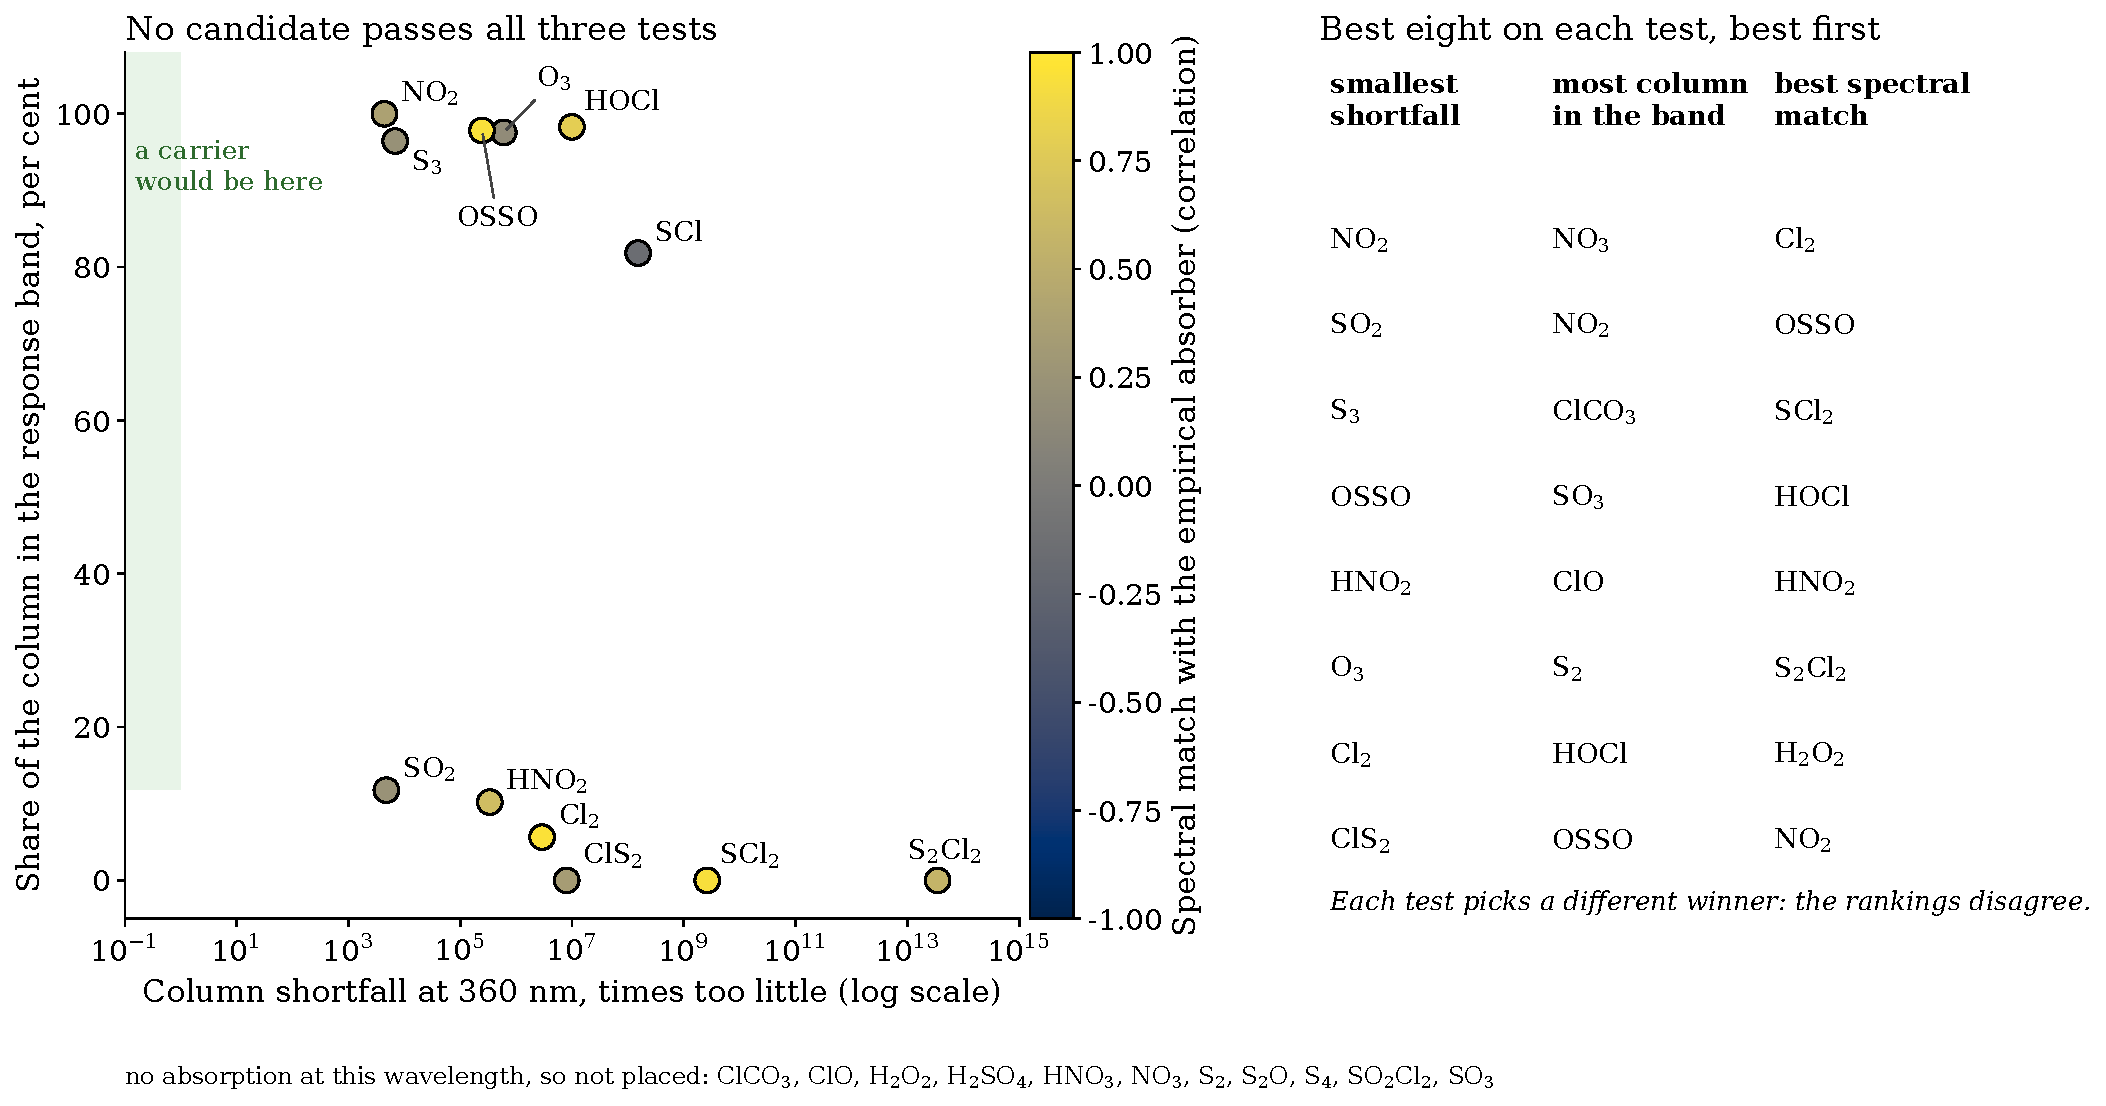
\includegraphics[width=\textwidth]{F15_E12_three-axis-screen_ch6_s14.pdf}
  \caption[The three-axis screen (Experiment~12)]{The three-axis screen (Experiment~12): shortfall at 360~nm (horizontal), share
    of the column in the response band (vertical) and spectral correlation (colour). A
    carrier would sit in the shaded corner, with no shortfall and most of its column in
    the band; species that do not absorb at 360~nm are listed below the axis. The right
    panel lists the best eight species on each test. Keys \texttt{e12.X.short.360},
    \texttt{e12.X.frac\_in\_band\_pct} and \texttt{e12.X.corr}, where X is the species.}
  \label{fig:F15}
\end{figure}

\textbf{Result.} Table~\ref{tab:screen} gives every species. Sixteen species pass on
placement and five on spectrum. Two pass both, OSSO
and HOCl, yet in amount they are short by $2.4563\times10^{5}$ and $9.9572\times10^{6}$. None passes on amount, so none passes all three
(Figure~\ref{fig:F15}; keys \texttt{e12.gate.n\_placement}, \texttt{e12.gate.n\_spectrum},
\texttt{e12.gate.n\_all}, \texttt{e12.S2O2.short.360} and \texttt{e12.HOCl.short.360}). The tests also
disagree about which species is ``best''. NO\sub{2} is the least short, by a factor of
4402.887 (key \texttt{e12.best\_shortfall}), and has 99.998\% of its column in the band, but peaks at
430~nm with a correlation of only 0.3862. HNO\sub{2} has the most absorption inside 320 to
400~nm, 98.031\%, but only 10.216\% of its column in the band. Cl\sub{2} correlates best,
at 0.9461, with 5.647\% in the band. No single ``most likely'' ranking exists.

\begin{table}[htbp]
  \centering
  \caption[The three-axis screen for all 23 species (Experiment~12), ordered by shortfall]{The three-axis screen for all 23 species (Experiment~12), ordered by shortfall.
    Shortfall: times too little at 360~nm above 69~km (``none at 360~nm'': the species does
    not absorb there). In band: per cent of the column above 58~km that lies in the
    response band. Share: per cent of the absorption between 300 and 698~nm that lies in
    320 to 400~nm. Pass marks: shortfall at most 1; in band at least 11.92 per cent; share
    above 50 per cent with correlation above 0.5. Keys \texttt{e12.<species>.short.360},
    \texttt{.frac\_in\_band\_pct}, \texttt{.share\_320\_400\_pct}, \texttt{.corr} and
    \texttt{e12.gate.*}.}
  \label{tab:screen}
  \footnotesize
  \setstretch{1.0}
  \begin{tabular}{lccccl}
    \toprule
    Species & Shortfall & In band (\%) & Share (\%) & Correlation & Passes on \\
    \midrule
    NO\sub{2} & $4.403\times10^{3}$ & 99.998 & 36.140 & $0.386$ & placement \\
    SO\sub{2} & $4.769\times10^{3}$ & 11.772 & 4.272 & $0.239$ & none \\
    S\sub{3} & $6.859\times10^{3}$ & 96.447 & 56.926 & $0.225$ & placement \\
    OSSO & $2.456\times10^{5}$ & 97.835 & 64.275 & $0.939$ & placement, spectrum \\
    HNO\sub{2} & $3.384\times10^{5}$ & 10.216 & 98.031 & $0.646$ & spectrum \\
    O\sub{3} & $6.012\times10^{5}$ & 97.570 & 5.606 & $0.169$ & placement \\
    Cl\sub{2} & $2.910\times10^{6}$ & 5.647 & 73.719 & $0.946$ & spectrum \\
    ClS\sub{2} & $8.010\times10^{6}$ & $1.3\times10^{-4}$ & 60.673 & $0.342$ & none \\
    HOCl & $9.957\times10^{6}$ & 98.295 & 52.967 & $0.796$ & placement, spectrum \\
    SCl & $1.523\times10^{8}$ & 81.836 & 14.474 & $-0.156$ & placement \\
    SCl\sub{2} & $2.618\times10^{9}$ & $2.3\times10^{-3}$ & 71.043 & $0.936$ & spectrum \\
    S\sub{2}Cl\sub{2} & $3.469\times10^{13}$ & $5.0\times10^{-6}$ & 32.933 & $0.570$ & none \\
    ClCO\sub{3} & none at 360~nm & 99.981 & 0 & $0.225$ & placement \\
    ClO & none at 360~nm & 99.332 & 4.121 & $0.159$ & placement \\
    H\sub{2}O\sub{2} & none at 360~nm & 58.857 & 27.559 & $0.484$ & placement \\
    H\sub{2}SO\sub{4} & none at 360~nm & 0.969 & 0 & $-0.218$ & none \\
    HNO\sub{3} & none at 360~nm & 34.902 & 6.619 & $0.215$ & placement \\
    NO\sub{3} & none at 360~nm & 100.000 & 0 & $-0.519$ & placement \\
    S\sub{2} & none at 360~nm & 98.741 & 0.167 & $0.253$ & placement \\
    S\sub{2}O & none at 360~nm & 50.181 & 4.159 & $0.239$ & placement \\
    S\sub{4} & none at 360~nm & 97.261 & 0 & $-0.304$ & placement \\
    SO\sub{2}Cl\sub{2} & none at 360~nm & 35.317 & 0 & $-0.039$ & placement \\
    SO\sub{3} & none at 360~nm & 99.847 & 10.286 & $0.314$ & placement \\
    \bottomrule
  \end{tabular}
\end{table}

Amount is a gate, not a tie-breaker: the shortfalls run from thousands to about $10^{13}$,
while placement and spectrum were each worth less than a factor of ten.

% ===========================================================================
\section{Experiment 13: iron and sulfur minerals}
\label{sec:e13}

\textbf{Question and design.} Jiang et al.\ proposed rhomboclase and acid ferric sulfate
from their spectral shape~\cite{jiang2024}. Spacek et al.\ later derived how strongly the
droplet liquid must absorb: a decadic coefficient of 1278 per centimetre at
375~nm~\cite{spacek2026}. Nobody had put the two together. Using the mass extinction
coefficients measured by Jiang et al.\ and the straight-line scaling of Spacek et al., the
mass of mineral needed per litre of droplet is the requirement divided by the coefficient:
\begin{equation}
  m = \frac{a_{\mathrm{req}}}{\varepsilon} , \qquad s = 100\,\frac{m}{\rho} ,
  \label{eq:loading}
\end{equation}
where $a_{\mathrm{req}} = 1278$ per centimetre is the required decadic coefficient at
375~nm (\texttt{e13.A\_required}), $\varepsilon$ is the material's mass absorption
coefficient at 375~nm in square centimetres per gram, $m$ is the mass needed in grams per
cubic centimetre, which is the same number in kilograms per litre, and $s$ is that mass
as a share of the 1.8~kg that a litre of droplet liquid weighs, the droplet density used
by Dai et al.~\cite{dai2023kzz} (\texttt{e13.rho\_solution}).
For rhomboclase $\varepsilon$ is 422.797 and for acid ferric sulfate 293.144
(\texttt{e13.X.eps\_375}); for ferric chloride in water, 1~g per litre gives about 1 per
centimetre, so $\varepsilon$ is 1000.
The script first reproduces the ferric chloride figure of Spacek et al.\ from their
stated input, 1.278 against their 1.3~kg per litre (\texttt{e13.fecl3.loading\_kg\_per\_L});
that line is a check on the method, never a result about ferric chloride.

\begin{figure}[tbp]
  \centering
  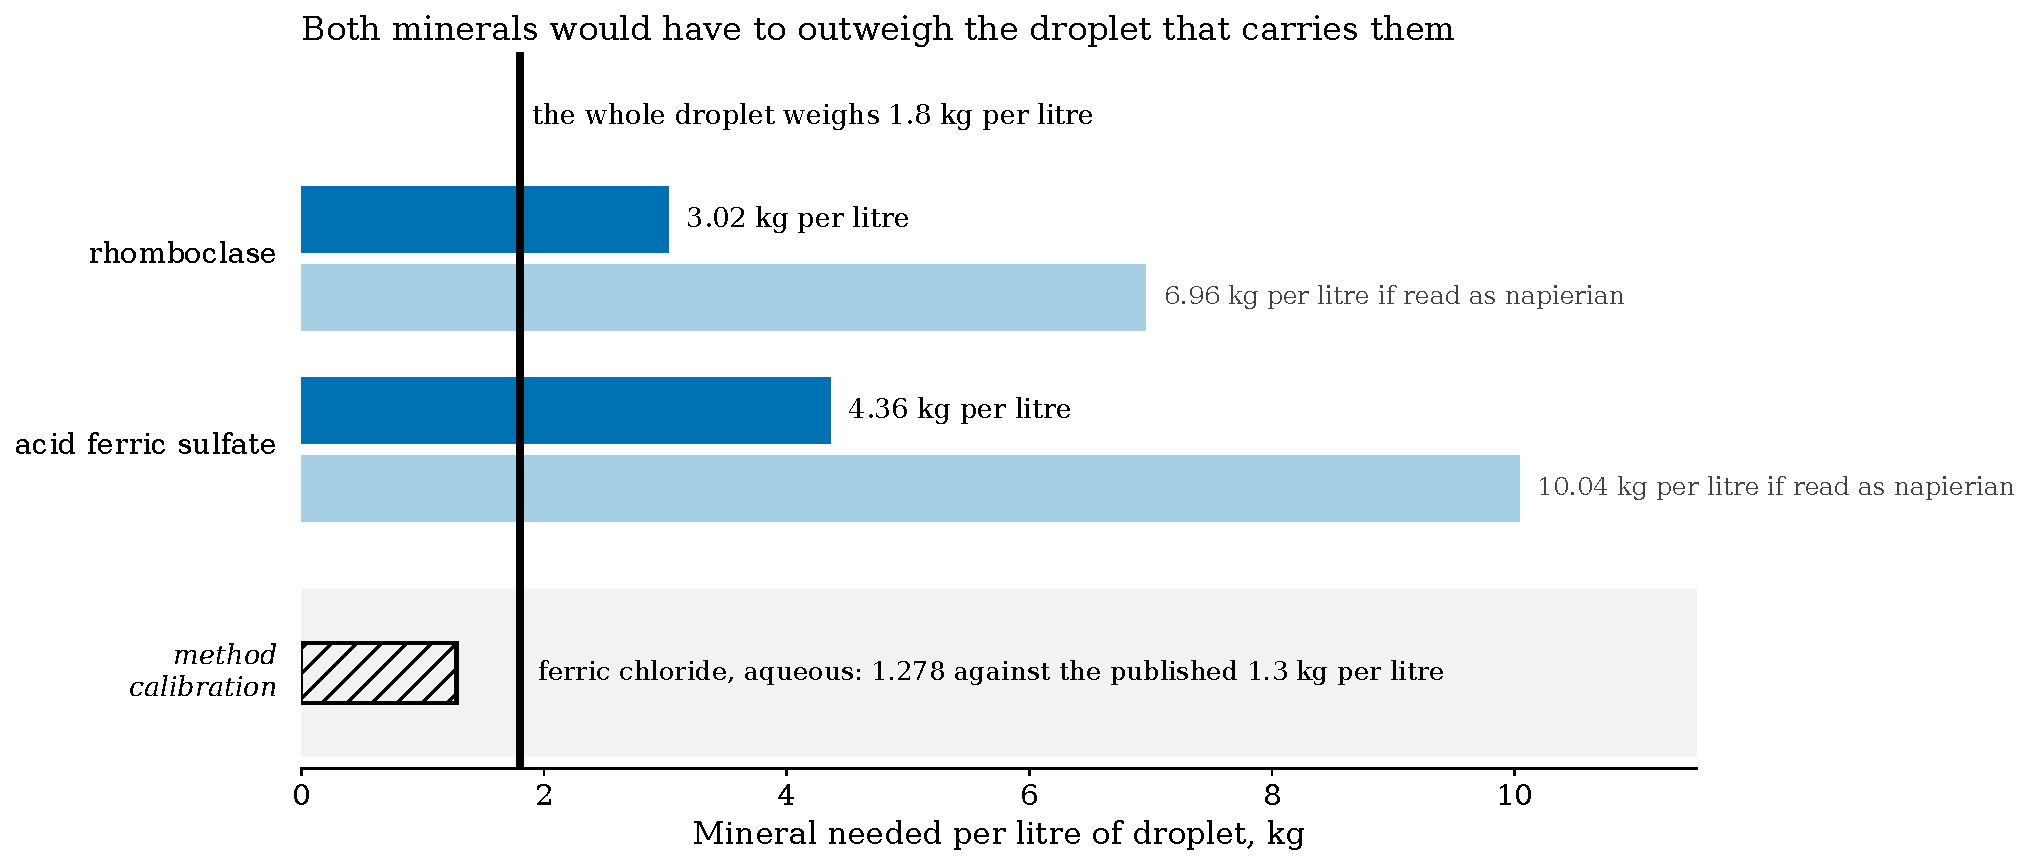
\includegraphics[width=0.9\textwidth]{F16_E13_minerals-cannot-reach_ch6_s15.pdf}
  \caption[Mineral needed per litre of droplet (Experiment~13)]{Mineral needed per litre of droplet to meet the requirement at 375~nm
    (Experiment~13); dark bars read the coefficients as decadic, light bars as natural
    (Napierian), the vertical line is the mass of a litre of droplet and the hatched
    bar is the calibration. Keys \texttt{e13.rhomboclase.*},
    \texttt{e13.acid\_ferric\_sulfate.*} and \texttt{e13.fecl3.*}.}
  \label{fig:F16}
\end{figure}

\textbf{Result.} Rhomboclase would need 3.02~kg per litre, 167.93\% of the droplet's own
mass, and acid ferric sulfate would need 4.36~kg per litre, 242.20\% (keys
\texttt{e13.X.pct\_of\_droplet}, where X is the mineral), against a droplet
density of 1.8~kg per litre (Figure~\ref{fig:F16}). At 375~nm, even a droplet made
entirely of either mineral could not absorb enough. Reading the coefficients as natural
rather than decadic raises the need to 6.96 and 10.04~kg per litre. At each mineral's own
absorption peak the need is 156.43\% and 95.07\% of the droplet mass
(\texttt{e13.X.pct\_at\_peak}): rhomboclase still cannot reach it, and acid ferric sulfate
could only as a droplet almost wholly made of the mineral.
The verdict is also conservative: the coefficients were measured through a suspension and
include scattering, and removing it can only raise the mass needed.

% ===========================================================================
\section{Experiment 14: ferric chloride measured in acid}
\label{sec:e14}

Experiment~14 was done after Phase~1 closed; it is reported because it changes how a
published result should be read.

\textbf{Question and design.} Spacek et al.\ find the absorbance of ferric chloride too
low, because it would need about 1.3~kg per litre~\cite{spacek2026}; the method of
Experiment~13 gives 1.278~kg per litre from the same input, which with the droplet density
is 71.0\% of the droplet mass (\texttt{e14.aqueous\_pct\_of\_droplet}). Their input
is an absorbance measured in water. Egan et al.\ note that the solvent has a significant
effect on the spectrum of ferric chloride, and derived its molar absorptivity in
hydrochloric acid at five strengths, from 1.54 to 12.2 moles per litre, labelling the
curves Cl~A to Cl~E; they use these curves as the ferric chloride components when they
fit their mixed sulfuric and hydrochloric acid samples~\cite{egan2025lab}. One script read those five curves
from the published figure at 600 dots per inch and writes nothing unless three checks
pass. The first finds the frame of the left panel, so that every point is measured from
the true axes. The second requires the tick marks to be evenly spaced to better than
1\% on both axes, so that the scale has been read without stretching. The third requires
every curve to fall back to zero at its long-wavelength end, so that the vertical zero is
where the figure puts it. To test the checks, the zero was deliberately shifted; the
third check first let the shift through, and was tightened to a tenth of a tick until it
caught it. A second script reproduces the figure of Spacek et al.\ from their aqueous input,
1.278 against their 1.3~kg per litre, then repeats Equation~\eqref{eq:loading} with the five hydrochloric acid values.

\begin{figure}[tbp]
  \centering
  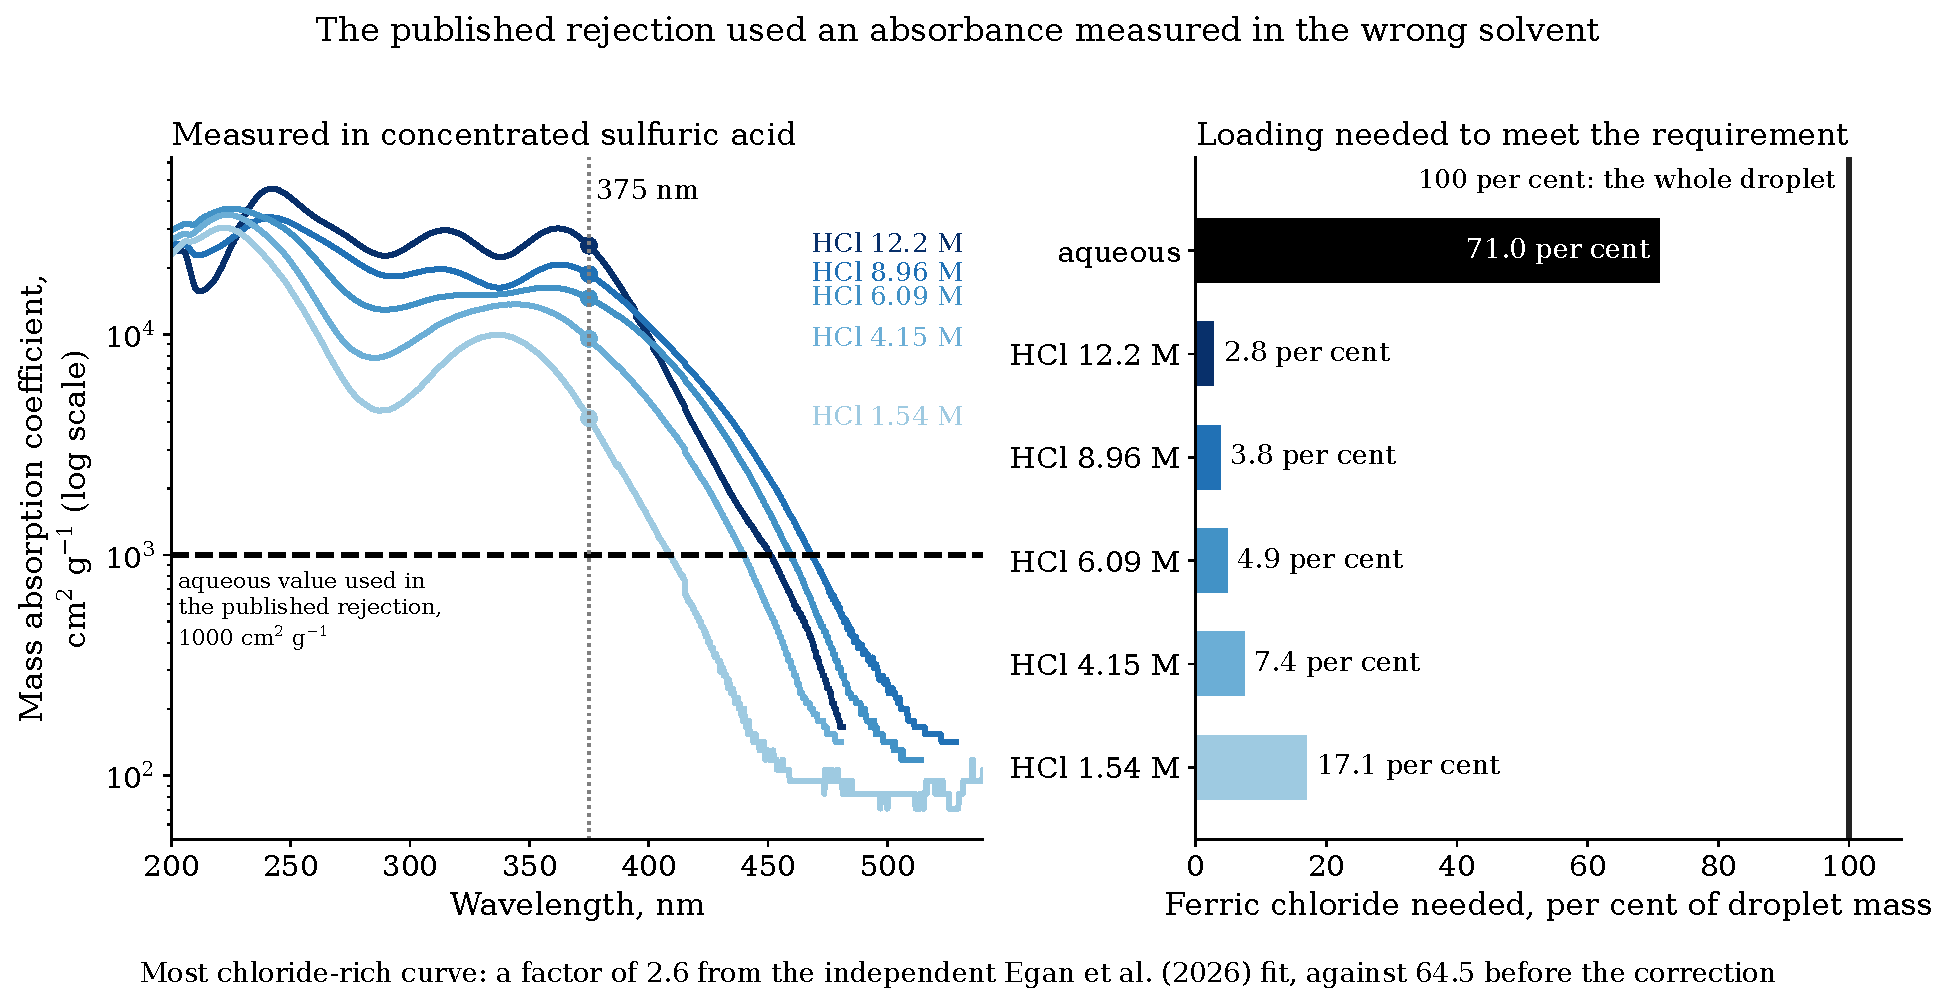
\includegraphics[width=\textwidth]{F17_E14_ferric-chloride-correction_ch6_s16.pdf}
  \caption[Ferric chloride in hydrochloric acid and the loading each curve needs (Experiment~14)]{Ferric chloride in hydrochloric acid at five strengths (left, read from Egan
    et al.~\cite{egan2025lab}) and the loading each needs as a share of the droplet mass
    (right), against the aqueous value of the published rejection (Experiment~14). The
    curves are those of their Figure~5a. Keys
    \texttt{e14.ClA.*} to \texttt{e14.ClE.*} and \texttt{e14.factor\_to\_fit\_after}.}
  \label{fig:F17}
\end{figure}

\textbf{Result.} In these solutions, ferric chloride absorbs 4.164 to 25.192 times more
strongly at 375~nm than the aqueous value (\texttt{e14.ratio\_lo},
\texttt{e14.ratio\_hi}). The loading needed falls from 1.278~kg per litre to between
0.0507 and 0.3069, that is from 71.0\% of the droplet mass to between 2.82\% and 17.05\%
(\texttt{e14.ClA.pct\_of\_droplet}, \texttt{e14.ClE.pct\_of\_droplet};
Figure~\ref{fig:F17}). If ferric chloride in the droplets absorbs as it does in any of
these solutions, the rejection does not survive: even the weakest curve leaves it a
plausible minor component. The answer is a range because the iron forms several chloride
complexes whose shares depend on the chloride available, and how much chloride the
droplets hold is not settled here. Table~\ref{tab:e14} shows the trend: the more hydrochloric acid in
the solution, the more strongly ferric chloride absorbs at 375~nm and the less of it is
needed.

\begin{table}[htbp]
  \centering
  \caption[The five ferric chloride curves at 375~nm (Experiment~14)]{The five ferric chloride curves of Egan et al.~\cite{egan2025lab} at 375~nm,
    and the loading each needs by Equation~\eqref{eq:loading} (Experiment~14). Molar
    $\varepsilon$ in litres per mole per centimetre, mass $\varepsilon$ in square
    centimetres per gram; share of the droplet's own mass. Keys
    \texttt{e14.<curve>.hcl\_M}, \texttt{.eps\_molar}, \texttt{.eps\_mass},
    \texttt{.loading\_kg\_per\_L} and \texttt{.pct\_of\_droplet}.}
  \label{tab:e14}
  \footnotesize
  \setstretch{1.0}
  \begin{tabular}{lccccc}
    \toprule
    Curve & HCl (mol/L) & $\varepsilon$, molar & $\varepsilon$, mass & Loading (kg/L) &
      Share (\%) \\
    \midrule
    Cl~A & 12.20 & 4086.212 & 25191.806 & 0.0507 & 2.82 \\
    Cl~B & 8.96 & 3036.595 & 18720.842 & 0.0683 & 3.79 \\
    Cl~C & 6.09 & 2362.116 & 14562.626 & 0.0878 & 4.88 \\
    Cl~D & 4.15 & 1546.601 & 9534.912 & 0.1340 & 7.45 \\
    Cl~E & 1.54 & 675.439 & 4164.130 & 0.3069 & 17.05 \\
    \bottomrule
  \end{tabular}
\end{table}

The correction also brings two 2026 papers that do not cite each other closer. The
preprint of Egan et al., not peer reviewed, fits 1.0 to 1.2~wt\% ferric chloride in the
smallest droplets to the MESSENGER spectrum~\cite{egan2026}. The most chloride-rich curve
here needs 2.82\%, a factor of 2.6 from the middle of that range
(\texttt{e14.factor\_to\_fit\_after}), against 64.5 before. The two figures still rest on
different assumptions: Spacek et al.\ spread the absorber through two droplet sizes in a
layer near the cloud top, while the preprint puts it in the smallest droplets only, which
also reach higher into the haze. Spacek et al.\ note that either change would alter their
requirement, in opposite directions~\cite{spacek2026}, so the remaining factor of 2.6 is
not a contradiction, but it is not yet explained.

\textbf{What Experiment 14 does not claim.} It corrects one input to another group's
argument. It does not identify the absorber, and nothing in it measures Venus. The
laboratory spectra were taken far more dilute than these loadings and are scaled in a
straight line, as Spacek et al.\ also do. Above all, ferric chloride has not been tested
on altitude, the test that decided Experiment~9, because it has no chemistry in the model
and so cannot be placed by it. That test belongs to Phase~2 (Chapter~9).

% ===========================================================================
\section{What Experiments 8 to 14 establish}
\label{sec:e814-summary}

\begin{itemize}
  \item Placement matters more than spectral shape, 7.34 against 4.95, and shape matters
    only where the absorber overlaps the responding layer.
  \item Placed by the model's own chemistry, the closest gas-phase candidate falls out of
    the response band and becomes radiatively the same as no absorber.
  \item Two runs that should agree give radiation fields that differ by 0.0017\% of the
    change they make, but change the SO abundance in the band by 0.7384\% and 2.5278\%
    from the same baseline. An apparent
    fingerprint was linear response and has been withdrawn.
  \item No species the model can represent passes amount, placement and spectrum together,
    and the three tests disagree about which comes closest.
  \item At 375~nm the proposed iron and sulfur minerals cannot absorb enough even as
    pure solids. Ferric chloride, rejected on an aqueous measurement, becomes a plausible
    minor component if it absorbs in the droplets as it does in hydrochloric acid, but
    its altitude is untested.
\end{itemize}

% ===========================================================================
% Chapter 7: What Phase 1 establishes, and its limits
% ===========================================================================
\chapter{What Phase 1 Establishes}
\label{ch:establish}

This chapter states what the fourteen experiments establish and within which limits.
\emph{Measured} marks a claim resting on radiative comparisons, reproducible to 0.0017\%
of the change itself;
\emph{bounded} marks one resting on abundances, reproducible only to 2.5278\%
(Experiment~10).

\section{Established results}
\label{sec:est-results}

\textbf{The absorber term works, and its effect is located (measured).} The model's
absorber changes the radiation field in proportion to its amount, locally in wavelength,
and within one band of altitude, 69 to 93~km (Chapter~\ref{ch:exp17}).

\textbf{Placement is a first-order control (measured).} The same absorber has 7.34 times
more effect moved up than moved down, while changing its spectrum at a fixed placement is
worth a factor of 4.95, and spectral shape stops mattering once the absorber leaves the
responding layer (Experiments~7, 8 and~10).

\textbf{The chemistry, not the modeller, decides placement, and the closest gas-phase
candidate fails on it (measured).} At the profile its own chemistry gives it, ClS\sub{2}
leaves the response band and the radiation field becomes that of no absorber, to
0.001487\% (\texttt{id.l2\_ratio\_pct}; Experiment~9).

\textbf{No species the model can represent passes all three tests (calculated from
saved model output).} The
screen uses only saved model output and stored cross sections (Experiment~12).

\textbf{Two published candidates are reassessed (calculated from published data).} The
proposed iron and sulfur minerals cannot absorb enough at 375~nm even as pure solids,
and the published rejection of ferric chloride does not survive if ferric chloride absorbs
in the droplets as it does in hydrochloric acid (Experiments~13 and~14). Neither result uses the model, and neither identifies the
absorber.

\textbf{The chemical responses are small and mostly unresolved (bounded).} Apart from SO
and SO\sub{3} when the absorber is moved up, by 8.404\% and 4.718\% (keys
\texttt{res.e7a.SO.inband} and \texttt{res.e7a.SO3.inband}), the changes in the sulfur
reservoirs inside the band are at or below the chemistry floor, or above it by too little
to settle anything (SO in Experiments~3 and~4B), and are reported only as upper bounds.

\section{Limits}
\label{sec:limits}

\begin{enumerate}[leftmargin=*, itemsep=2pt]
  \item \textbf{One column, one sun angle.} The model is a single global average at a
    zenith angle of 58 degrees, with every photolysis rate halved for day and night
    (Table~\ref{tab:setup}). Latitude and local time are not represented, and every run
    is a steady state.
  \item \textbf{Low vertical mixing.} Every run uses the Bierson and Zhang mixing
    profile~\cite{bierson2020}, orders of magnitude below what has since been derived
    for the clouds from observations and models~\cite{dai2023kzz, lefevre2024}. The vertical wind is switched off. The
    placement verdict of Experiment~9 has therefore been tested at one mixing strength
    only; Chapter~\ref{ch:phase2} proposes to test it at others.
  \item \textbf{Simplified cloud droplets.} The cloud droplets enter the radiation only
    through fixed, fitted cross sections for two droplet modes; the full droplet
    calculation in the code stays switched off in every run
    (Section~\ref{sec:discovery}).
  \item \textbf{An empirical reference.} The empirical absorber's spectrum and profile
    were fitted to the observed brightness of Venus. Spectral rankings measure resemblance
    to that fit, not correctness (Experiments~8 and~11).
  \item \textbf{Only what the network contains.} The screen can judge only species the
    model tracks and holds cross sections for: 23 of 62. Ferric chloride and the iron
    minerals have no chemistry in the model and could not be placed by it.
  \item \textbf{A floor from one pair.} The chemistry floor comes from a single pair of
    replicate runs and is a lower bound on the true numerical scatter
    (Section~\ref{sec:conv-floor}).
\end{enumerate}

None of these limits weakens a comparison between two runs, which share them; they
limit how far the verdicts carry to the real atmosphere, and the first two are the
subject of Phase~2.

% ===========================================================================
% Chapter 8: Verification
% ===========================================================================
\chapter{Verification}
\label{ch:verify}

No number in this report was typed in by hand. This chapter shows how numbers are
produced and checked, how to read a registry key, and what the checks catch.

% ===========================================================================
\section{The registry and its keys}
\label{sec:keys}

The script \texttt{verify/recompute\_25m0328.py} reads the model output committed to the
repository, recomputes every quantity the project uses, and writes them to
\texttt{verify/registry.json}: 10830 named values in 71 groups. Anyone can rebuild it
from the committed output by running the script, which also states the conventions of
Chapter~\ref{ch:conv}.

Each value has a \emph{key}: parts separated by full stops, read from left to right,
from the general to the particular,
\emph{group}\,.\,\emph{case or species}\,.\,\emph{quantity}\,.\,\emph{qualifier}. The
group names the source, usually an experiment; the middle parts narrow it to one run,
species, reaction or window; the last part names the quantity and, where needed, a
wavelength or a unit. Not every key has all four parts. Table~\ref{tab:keygroups} lists
the groups quoted in this report, and Appendix~\ref{app:filemap} lists, for each
experiment, its run files, scripts and registry groups.

\begin{table}[htbp]
  \centering
  \caption[Registry groups quoted in this report]{Registry groups quoted in this report.}
  \label{tab:keygroups}
  \footnotesize
  \setstretch{1.0}
  \begin{tabularx}{\textwidth}{>{\raggedright\arraybackslash}p{3.3cm}
                                >{\raggedright\arraybackslash}X}
    \toprule
    Group & What it holds \\
    \midrule
    \texttt{e1} to \texttt{e14} & One experiment each; letters mark a case or sub-study
      (\texttt{e7a} is Experiment~7A, \texttt{e3fp} the whole-field test of Experiment~3 at all four amplitudes) \\
    \texttt{res} & Largest change in a sulfur reservoir species, per case \\
    \texttt{dJ}, \texttt{dJy}; \texttt{dJz}, \texttt{dJyz} & Photolysis change as
      $\Delta J$ and as $\Delta(Jn)$; the heights where each peaks \\
    \texttt{nom}, \texttt{conv} & Reference and baseline runs; steady-state tests \\
    \texttt{pnom}, \texttt{p9}, \texttt{spec\_*}, \texttt{tau} & Absorber profiles,
      spectra, and optical depths built from them \\
    \texttt{scr}, \texttt{iso}, \texttt{corr} & Experiment~8 screen, Experiment~11
      isomers, spectral correlations \\
    \texttt{five}, \texttt{share320400} & Comparison of the five spectra; share of
      absorption between 320 and 400~nm \\
    \texttt{falselead} & The optical depths of the false lead (Chapter~3) \\
    \texttt{id}, \texttt{chr}, \texttt{chr8}, \texttt{twoby2}; \texttt{const},
      \texttt{p2} & Tests of
      Experiments~9 and~10; fixed constants; Phase~2 mixing times \\
    \bottomrule
  \end{tabularx}
\end{table}

\textbf{Example 1.} \texttt{e12.S2O2.short.360}: Experiment~12; species S\sub{2}O\sub{2}
(OSSO); shortfall factor; at 360~nm. Its value, $2.4563\times10^{5}$: the model holds that many
times too little OSSO above 69~km.

\textbf{Example 2.} \texttt{res.e7a.SO.inband}: reservoir responses; case 7A, the absorber
moved up; species SO; largest relative change inside the response band. Its value,
8.404\%, is one of the two abundance changes above the chemistry floor.

\textbf{Example 3.} \texttt{e7.7a.SO2.R781.col} and its twin ending \texttt{col\_km}:
Experiment~7; case 7A; species SO\sub{2}; reaction R781; the column-integrated change in
its rate, with thickness in centimetres, $8.2352\times10^{8}$, and in the old, wrong,
kilometre form, 8235.1671, kept to show the error (Section~\ref{sec:conv-col}).

\textbf{Example 4.} \texttt{e1.aflux.meanrel}: Experiment~1; actinic flux; mean relative
change. It is stored as the fraction $1.3553\times10^{-4}$ and printed as 0.013553\%. Keys
ending in \texttt{pct} hold percentages; keys ending in \texttt{rel} hold fractions.

% ===========================================================================
\section{The checker, and what it cannot catch}
\label{sec:checker}

The script \texttt{verify/check\_documents\_25m0328.py} finds every number in a document
written with three or more decimals, in scientific notation, or as a percentage with two
or more decimals, and accepts it only if a registry value, rounded to the number's own
significant digits, gives it (Section~\ref{sec:conv-numbers}). Three faults in the
checker (unbraced exponents, too tight a tolerance, DOIs read as numbers) were found
because it rejected correct numbers, and fixed. Chapters~1 to~10 of this report print
407 checked numbers and the twenty figures print 129 (checked by
\texttt{figures/check\_figures.py}); none is unmatched.

The checker proves that a number is in the registry, not that it came from the right
key. For example, \texttt{pnom.col\_dzw} holds $4.0775\times10^{8}$ per square
centimetre, which the checker would accept as the absorber column; but only
\texttt{pnom.column}, $4.0776\times10^{8}$, summed on the grid the absorber term uses,
reproduces $\tau_{\mathrm{req}}$. Every number in this report was therefore also
checked by hand against the key named beside it.

\textbf{Reproduction.} The eleven runs in the \texttt{conv} group, from the nominal run of
Experiment~2 to Experiment~11, all ended with \texttt{longdy} between 0.0097778 and
0.0099988, below the limit of 0.01. The registry can be rebuilt by anyone from the
committed output with \texttt{verify/recompute\_25m0328.py}.

% ===========================================================================
\section{One number, traced from end to end}
\label{sec:trace}

Take the 7.34 of Experiment~7, the number this report quotes most often, and follow it
from the model to the page.

\begin{enumerate}[leftmargin=*, itemsep=2pt]
  \item \textbf{The model output.} Three runs saved in the repository's \texttt{output}
    folder: the upward move, \texttt{Experiment7A\_UUV-upward18-25m0328.vul}; the
    downward move, \texttt{Experiment7B\_UUV-downward18-25m0328.vul}; and the reference,
    \texttt{Experiment2\_A1\_UUV-nominal-25m0328.vul}, with the absorber in its usual
    place. Each file holds the actinic flux field of its run.
  \item \textbf{The calculation.} \texttt{verify/recompute\_25m0328.py} loads the three
    files and calls its function \texttt{radiative()} twice, once for each move against
    the reference. The function subtracts the two fields and evaluates
    Equation~\eqref{eq:field}.
  \item \textbf{The registry.} The results are stored as \texttt{e7a.L2pct} and
    \texttt{e7b.L2pct}, and their ratio, 7.3367, as \texttt{e7.ratio\_7A\_over\_7B}.
  \item \textbf{The sentence.} Section~\ref{sec:e7} prints 2.2498\% and 0.3067\% with
    those keys, and the ratio as 7.34.
  \item \textbf{The checker.} It finds 2.2498\% and 0.3067\% in the chapter and accepts
    each, because the registry value rounded to the same digits gives it. The ratio,
    printed with two decimals, falls outside the checker's rule, so it was checked by
    hand: 2.2498 divided by 0.30665 is 7.3367, which rounds to 7.34.
\end{enumerate}

Any number in this report can be followed the same way, backwards from the key printed
beside it.

% ===========================================================================
\section{What the checks catch}
\label{sec:errors}

Recomputing every number and checking every printed value guards against three kinds of
error, and each can be seen in the registry or the code. \textbf{Units}: an integral over
altitude taken with the thickness in kilometres is $10^{5}$ times too small; the registry
keeps both forms of one such integral, \texttt{e7.7a.SO2.R781.col} and
\texttt{e7.7a.SO2.R781.col\_km}, so the size of the error can be seen
(Section~\ref{sec:conv-col}). \textbf{The wrong key}: a number can be in the registry
and still answer a different question, which is why every sentence is also checked
against the key it names (Section~\ref{sec:checker}). \textbf{Reading below the floor}:
a change in abundance smaller than 2.5278\% is not a measurement, so it is reported only
as an upper bound (Section~\ref{sec:conv-floor}).

% ===========================================================================
% Chapter 9: Phase 2 proposal
% ===========================================================================
\chapter{Phase 2 Proposal}
\label{ch:phase2}

Phase~1 found that placement decides whether a candidate matters, but every run used one
weak description of vertical mixing (Chapter~\ref{ch:establish}). Phase~2
asks whether the verdict survives realistic transport and whether transport
can carry a candidate into the response band. It also takes up the detailed modelling of
ferric chloride, which the supervisor reserved for this phase.

% ===========================================================================
\section{The idea: fast winds, slow rising}
\label{sec:p2-idea}

The supervisor's direction, paraphrased: Venus rotates slowly, so its clouds are carried
round quickly while air rises slowly; if something from below reaches the cloud top and
absorbs ultraviolet light there, it should be looked for. A rough time for mixing to carry
a gas across a layer of thickness $L$ is $L^{2}/K_{zz}$, with $K_{zz}$ averaged over the
layer.

\begin{figure}[tbp]
  \centering
  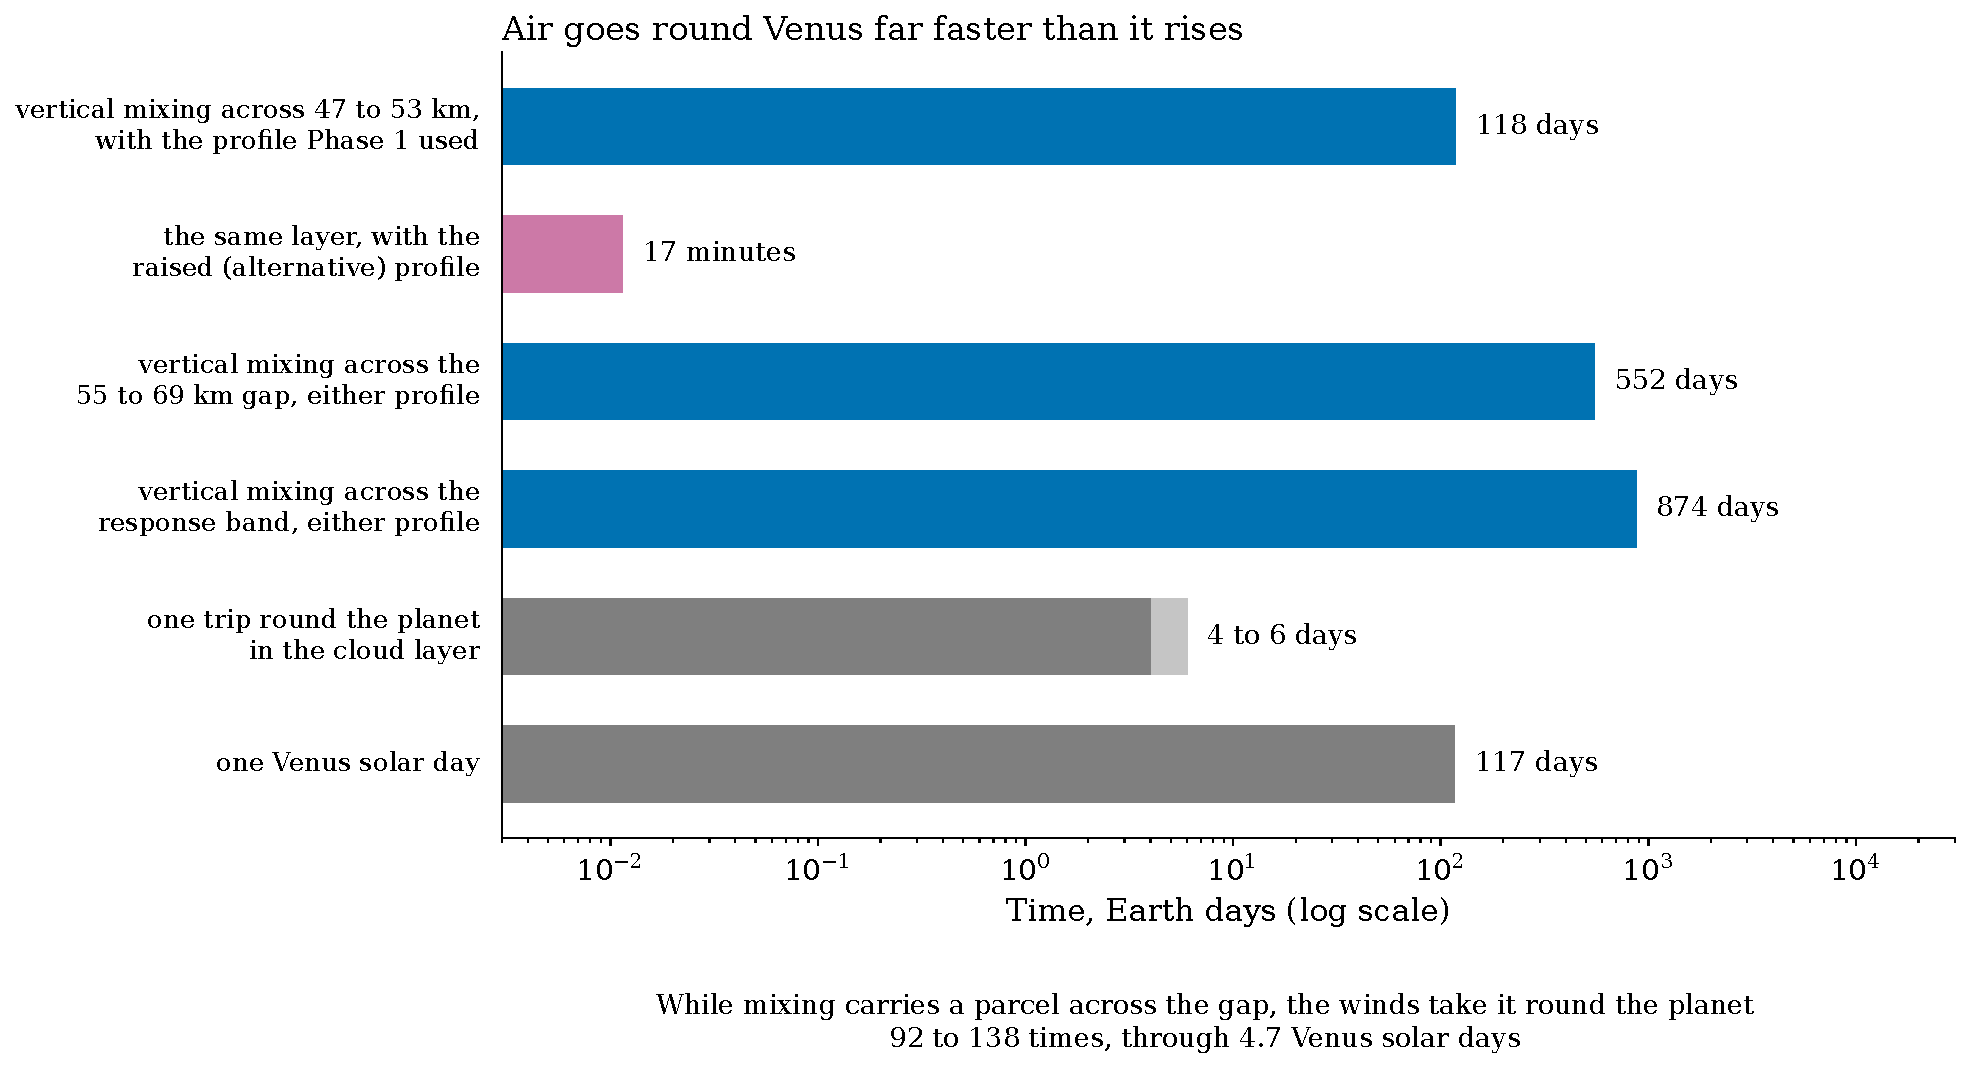
\includegraphics[width=0.7\textwidth]{F19_P2_transport-timescales_ch9_s19.pdf}
  \caption[Air goes round Venus far faster than it rises]{Air goes round Venus far faster than it rises. Mixing times $L^{2}/K_{zz}$
    across three layers, from the model's own mixing profiles, against the time for one
    trip round the planet~\cite{limaye2018} and one Venus solar
    day~\cite{bertaux2016}. Keys \texttt{p2.X.Bkzz.t\_days}, where X is the layer
    (\texttt{raised}, \texttt{gap} or \texttt{band}), and
    \texttt{p2.raised.BDkzz.t\_minutes}.}
  \label{fig:F19}
\end{figure}

Figure~\ref{fig:F19} shows the result. With the mixing profile of every Phase~1 run, a
gas needs about 552 days to cross the layer from 55 to 69~km (\texttt{p2.gap.Bkzz.t\_days})
and 874 days to cross the response band. The cloud layer goes round the planet in 4 to 6
days~\cite{limaye2018}, and one Venus solar day lasts 117 Earth
days~\cite{bertaux2016}. While mixing carries a parcel across the 55 to 69~km gap, the
winds take it round the planet 92 to 138 times, through 4.7 solar days. These times are
rough, but the contrast does not depend on the details.

% ===========================================================================
\section{What the literature adds}
\label{sec:p2-lit}

\textbf{The absorber is brought up, not made at the surface.} Bertaux et al.\ found that
the cloud-top wind and ultraviolet brightness at low southern latitudes vary with the
mountains of Aphrodite Terra below. Wind over the slopes launches gravity waves that
break just below the cloud top; where the wind speeds up, air must rise to make up for
it, and that upwelling brings the absorber to the cloud top. They also note that SO\sub{2}
falls from 150~ppmv at 54~km to 0.1 to 1~ppmv at the cloud top, so if the absorber comes
from SO\sub{2}, it ``must be produced inside the upper cloud, just below the cloud top
level''~\cite{bertaux2016}. The surface launches the waves; it does not supply the
molecule. Titov et al.\ tie the dark low-latitude markings to the same supply from
below~\cite{titov2008}.

\textbf{Mixing in the clouds is far stronger than Phase~1 assumed.} From Venus Express
sulfuric acid vapour, Dai et al.\ derived a global mean $K_{zz}$ peaking at
$5\times10^{8}$~cm$^{2}$\,s$^{-1}$ near 48~km and falling rapidly above
54~km~\cite{dai2023kzz}. Lef\`evre et al.\ found $10^{6}$ to $10^{8}$ in the 48 to 55~km
convective layer~\cite{lefevre2024}.

\textbf{A convective layer may sit inside the response band at noon.} In the model of
Lef\`evre et al., at the equator at noon, solar heating by the absorber itself drives a
convective layer at about 66 to 74~km, which the authors call still
speculative~\cite{lefevre2022}, overlapping the response band (Figure~\ref{fig:F20}). There,
a species whose chemical lifetime exceeds the 6000~s convective time becomes well
mixed~\cite{lefevre2022}. The authors note that the absorber's uncertain distribution ``could have a strong effect
on the cloud-top convection depth and vertical mixing'', and call for ``new 1D chemical
simulations with a more realistic convective mixing''~\cite{lefevre2022}. Phase~1 studied
exactly that distribution and its radiative effect.


\begin{figure}[tbp]
  \centering
  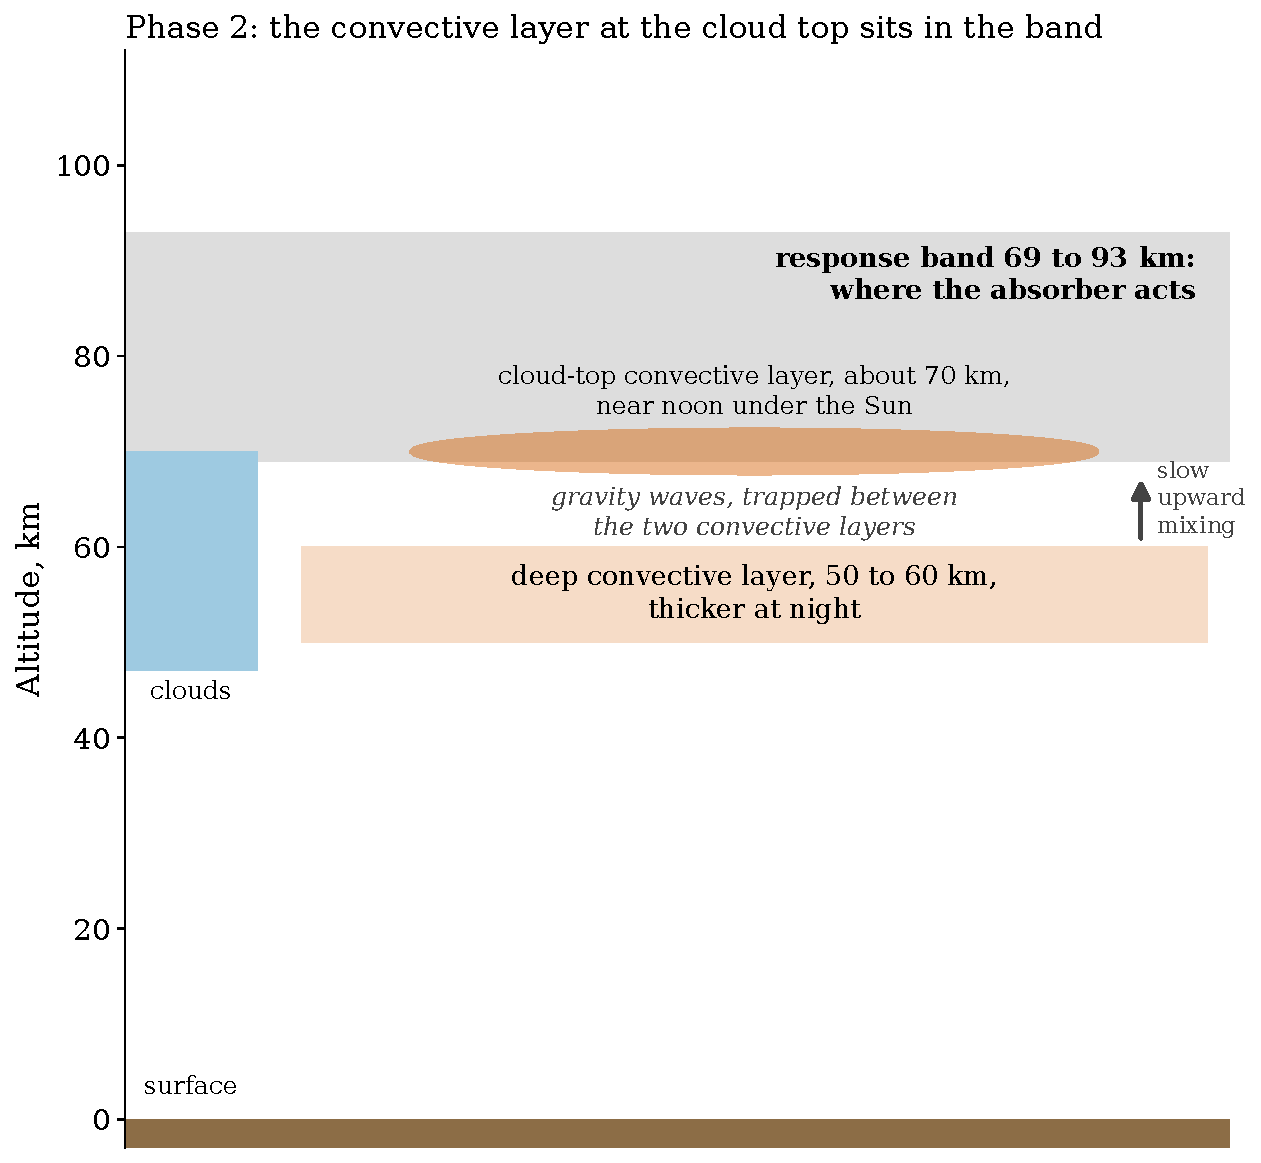
\includegraphics[width=0.7\textwidth]{F20_P2_altitude-map_ch9_s19.pdf}
  \caption[Where the layers sit]{Where the layers sit. The deep convective layer, 50 to 60~km in this study
    (other set-ups place it at 47 to 56 or 48 to 55~km, as above), is thicker at
    night; the cloud-top convective layer, near 70~km, appears at noon and lies inside
    the response band~\cite{lefevre2022}. Keys \texttt{e6.interval.90.lo} and
    \texttt{e6.interval.90.hi}.}
  \label{fig:F20}
\end{figure}

% ===========================================================================
\section{What the model already contains}
\label{sec:p2-model}

Three switches in the supplied code bear directly on Phase~2.

\textbf{A second mixing profile, never used.} The configuration file uses the mixing
in \texttt{atm/atm\_Venus\_Bkzz.txt}. A second file, named in a line that is commented
out, sits beside it: \texttt{atm/atm\_Venus\_B+Dkzz.txt}. The two are identical except at the four layers centred at
47 to 53~km, where the second is raised by 8716 to 14011 times
(\texttt{p2.kzz.raised.ratio\_min}, \texttt{.ratio\_max}) to the values of Dai et
al.~\cite{dai2023kzz} (Figure~\ref{fig:F18}). With it, the crossing time of that layer
falls from 118 days to 17 minutes. Every Phase~1 result was reached without this
enhancement. It stops at 53~km, so on its own it does not reach the band.

\begin{figure}[tbp]
  \centering
  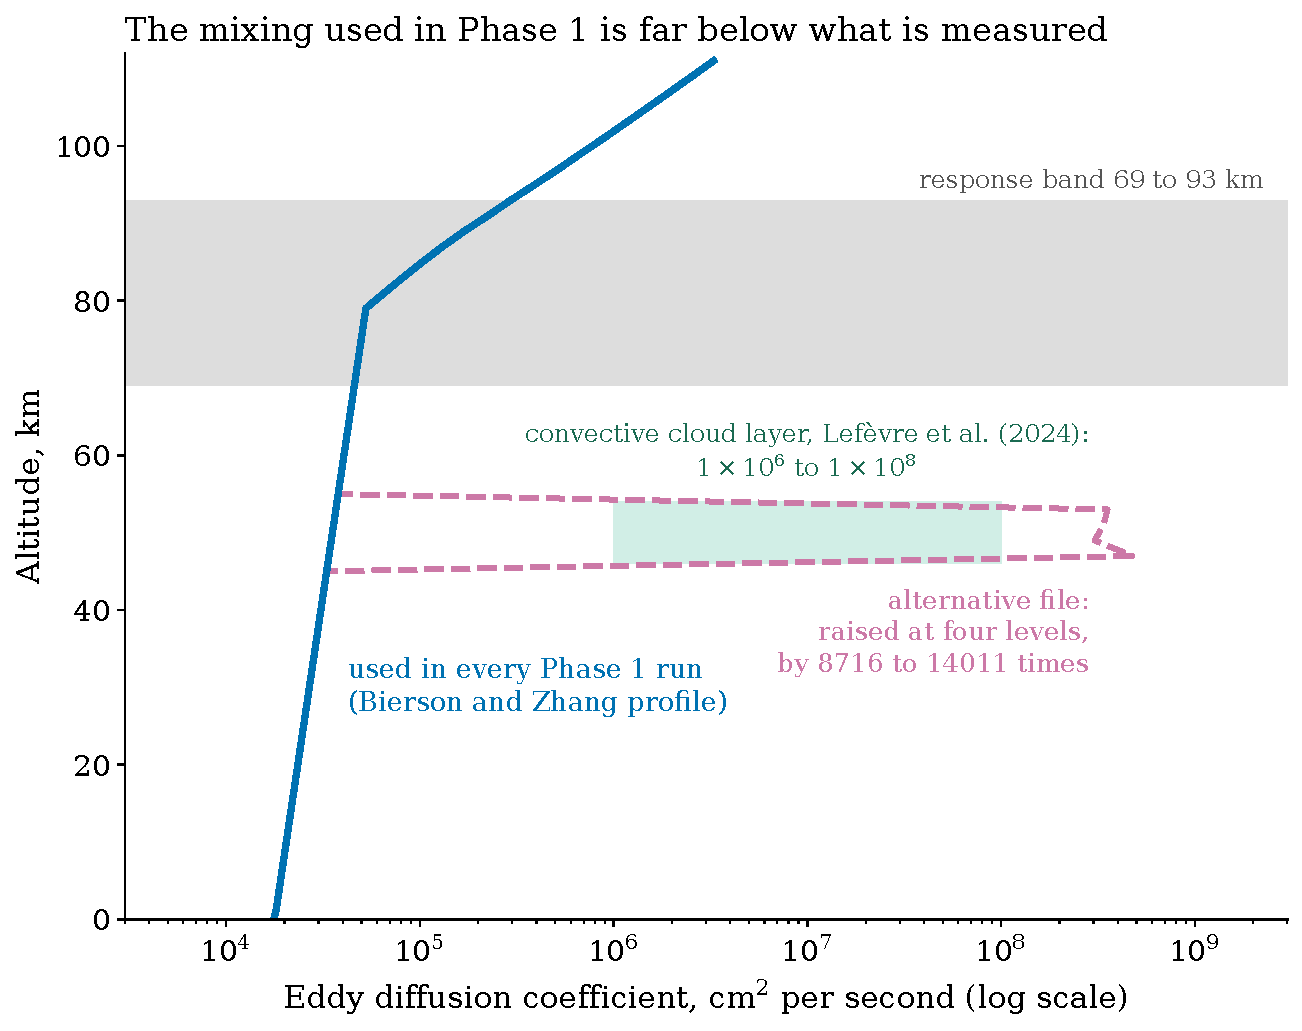
\includegraphics[width=0.7\textwidth]{F18_P2_two-mixing-profiles_ch9_report.pdf}
  \caption[The two mixing profiles supplied with the model]{The two mixing profiles supplied with the model. Solid: the profile of every
    Phase~1 run~\cite{bierson2020}. Dashed: the unused file, raised at four layers.
    Shaded: the convective layer of Lef\`evre et al.~\cite{lefevre2024}. Keys
    \texttt{p2.kzz.raised.ratio\_min} and \texttt{p2.kzz.raised.ratio\_max}.}
  \label{fig:F18}
\end{figure}


\textbf{Vertical wind, coded but off.} \texttt{use\_vz} is \texttt{False}, but upwind
advection is coded in \texttt{op.py}, and \texttt{build\_atm.py} can read a velocity per
level from a file.
\textbf{Day and night as two numbers.} Photolysis is halved (\texttt{f\_diurnal}) at one
zenith angle of 58 degrees (\texttt{sl\_angle}), untested for a noon-only layer.

% ===========================================================================
\section{Work packages}
\label{sec:p2-wp}

Each work package below is set out the same way: what changes in the model, what is
measured, what the result would mean, and what it needs first. Every measurement uses a
quantity Phase~1 already computes, so the registry and checker carry over unchanged.

\newpage
\textbf{WP1. Does the Phase~1 verdict survive stronger mixing?}
\nopagebreak[4]
\begin{itemize}[leftmargin=*, itemsep=1pt, topsep=2pt]
  \item \emph{Changes:} the mixing file named in \texttt{vulcan\_cfg.py}, switched to the
    raised profile of Section~\ref{sec:p2-model}; then a sweep of $K_{zz}$ from $10^{4}$
    to $10^{8}$~cm$^{2}$\,s$^{-1}$ over 46 to 70~km.
  \item \emph{Measures:} each candidate's centroid, its share of the column in the
    response band, and $\Delta F$ (Equation~\eqref{eq:field}), with the existing
    registry script.
  \item \emph{Would mean:} if the centroids and shares hold, the placement verdict
    survives the largest uncertainty in transport; if a candidate rises into the band,
    it goes back to the amount test. Dai et al.\ found the raised profile's effect on
    abundances ``slight''~\cite{dai2024}; the new question is placement and radiation.
  \item \emph{Needs:} nothing new; the file and the code exist.
\end{itemize}

\textbf{WP2. A cloud-top convective layer in one dimension.}
\nopagebreak[4]
\begin{itemize}[leftmargin=*, itemsep=1pt, topsep=2pt]
  \item \emph{Changes:} a new $K_{zz}$ profile that adds the noon layer near 70~km at
    the strength reported by Lef\`evre et al.~\cite{lefevre2022, lefevre2024}, justified
    against their published values.
  \item \emph{Measures:} the quantities of WP1, and the placement screen of
    Experiment~12 rerun on the new output.
  \item \emph{Would mean:} whether mixing inside the band can hold a candidate there.
    This is the piece that reaches into the band.
  \item \emph{Needs:} WP1, so that the effect of the new layer is separated from that of
    stronger mixing lower down.
\end{itemize}

\textbf{WP3. Upwelling.}
\nopagebreak[4]
\begin{itemize}[leftmargin=*, itemsep=1pt, topsep=2pt]
  \item \emph{Changes:} \texttt{use\_vz} switched on, with a vertical velocity for each
    level read from a file by \texttt{build\_atm.py} and used by the upwind advection
    already coded in \texttt{op.py}.
  \item \emph{Measures:} the inverse question: the smallest upward speed over 55 to
    67~km that delivers each candidate into the band before its chemistry destroys it.
  \item \emph{Would mean:} compared with what wave-driven upwelling could
    supply~\cite{bertaux2016}, whether rising air can do what mixing cannot. A
    one-dimensional model cannot represent a wave breaking over a mountain, so this
    tests a necessary condition only.
  \item \emph{Needs:} the lifetimes of WP5; it runs alongside WP2.
\end{itemize}

\textbf{WP4. The subsolar column.}
\nopagebreak[4]
\begin{itemize}[leftmargin=*, itemsep=1pt, topsep=2pt]
  \item \emph{Changes:} \texttt{sl\_angle} and \texttt{f\_diurnal} set for a column
    under the noon Sun instead of the halved, averaged sunlight, with a second column
    without sunlight for midnight, both on the mixing of WP2.
  \item \emph{Measures:} the quantities of WP1 at noon against the global mean, and
    SO\sub{2} at noon against the observed noon decrease of SO\sub{2} that accompanies an
    increase of the absorber~\cite{lefevre2022}.
  \item \emph{Would mean:} whether a candidate that fails in the global mean passes
    where light, heating and mixing are strongest together.
  \item \emph{Needs:} WP2.
\end{itemize}

\textbf{WP5. A fourth test: lifetime against transport.}
\nopagebreak[4]
\begin{itemize}[leftmargin=*, itemsep=1pt, topsep=2pt]
  \item \emph{Changes:} nothing in the model; a read-only script over saved output.
  \item \emph{Measures:} each candidate's chemical lifetime at each height, from its
    loss terms in \texttt{chem\_funs.py} read as in Experiment~5, against the time to
    reach the band, $L^{2}/K_{zz}$ (Section~\ref{sec:p2-idea}), with the 6000~s
    convective time at 70~km~\cite{lefevre2022} as a mark.
  \item \emph{Would mean:} a fourth axis for the screen of Experiment~12, and the answer
    to why the chemistry keeps ClS\sub{2} low (Experiment~9).
  \item \emph{Needs:} the output of WP1.
\end{itemize}

\textbf{WP6. Ferric chloride.}
\nopagebreak[4]
\begin{itemize}[leftmargin=*, itemsep=1pt, topsep=2pt]
  \item \emph{Changes:} iron and chlorine chemistry added to the network (a meteoric
    iron source, reactions with hydrogen chloride, uptake into droplets), and the
    ferric chloride cross sections obtained from the laboratory group.
  \item \emph{Measures:} the placement test of Experiment~9 for ferric chloride: its
    centroid, its share in the band and $\Delta F$.
  \item \emph{Would mean:} whether ferric chloride sits where the absorber acts, the
    test that Experiment~14 could not make.
  \item \emph{Needs:} the transport framework of WP1 to WP4; some rate constants may not
    exist, which is why it comes last.
\end{itemize}

\textbf{Order and risks.} WP1 and WP5 come first and can give a publishable result on
their own; WP2 and then WP4 follow, WP3 alongside WP2, and WP6 last. Three risks are
stated now. The absorber's heating drives the mixing that would move it, so the test will
be run with the mixing that heating would give and without it, and both reported. The
ferric chloride preprint's group is active~\cite{egan2026}, so WP6 may be overtaken. And
the 55 to 69~km gap may prove uncrossable; if so, that is the result.

% ===========================================================================
% Chapter 10: Conclusion
% ===========================================================================
\chapter{Conclusion}
\label{ch:conclusion}

\section{Key Findings}
\label{sec:key-findings}

\textbf{The model's absorber had been switched off, and switching it on locates its
effect.} The absorber term of VULCAN-Venus was present but inactive. Once active, it
changes the radiation field in proportion to its amount, and the change lives in one band
of altitude, 69 to 93~km.

\textbf{Where an absorber sits matters more than its spectrum.} The same absorber has 7.34
times more effect moved up than moved down, against a factor of 4.95 for its spectrum at
a fixed height.

\textbf{The chemistry decides where a candidate sits.} Placed by the model's own
chemistry, ClS\sub{2}, the gas closest in amount, falls below the response band and
becomes radiatively the same as no absorber. Being made in the right amount and absorbing
at the right wavelengths is not enough; a candidate must also be in the right place.

\textbf{No species in the model passes all three tests.} Of 23 species that could be
screened, none supplies enough absorption, and the three tests disagree about which comes
closest.

\textbf{Two published candidates are reassessed.} The proposed iron and sulfur minerals
cannot absorb enough at 375~nm even as pure solids. The published rejection of ferric
chloride rests on a measurement in water; if ferric chloride absorbs in the droplets as in
hydrochloric acid, it is a plausible minor component, though its altitude is untested.

\textbf{Every number is verified.} The registry recomputes every quantity from the saved
output, the checker tests every printed number precise enough to test, and
Chapter~\ref{ch:verify} traces numbers to the code.

Phase~2 asks whether these verdicts survive the much stronger mixing now estimated for
the Venus clouds, and whether it can carry a candidate into the band.


% References, IEEE style, numbered in alphabetical order of first author.
% Each entry is copied from the paper itself.
% Numbering follows the order below.

\begin{thebibliography}{99}
\addcontentsline{toc}{chapter}{References}

\bibitem{bertaux2016}
J.-L. Bertaux, I. V. Khatuntsev, A. Hauchecorne, W. J. Markiewicz, E. Marcq,
S. Lebonnois, M. Patsaeva, A. Turin, and A. Fedorova, ``Influence of Venus topography
on the zonal wind and UV albedo at cloud top level: the role of stationary gravity
waves,'' \emph{Journal of Geophysical Research: Planets}, vol. 121, pp. 1087 to 1101,
2016, doi: 10.1002/2015JE004958.

\bibitem{bierson2020}
C. J. Bierson and X. Zhang, ``Chemical cycling in the Venusian atmosphere: a full
photochemical model from the surface to 110 km,'' \emph{Journal of Geophysical Research:
Planets}, vol. 125, art. e2019JE006159, 2020, doi: 10.1029/2019JE006159.

\bibitem{dai2023kzz}
L. Dai, W. Shao, H. Gu, and Z. Sheng, ``Determination of the eddy diffusion in the
Venusian clouds from VeRa sulfuric acid observations,'' \emph{Astronomy and
Astrophysics}, vol. 679, art. A155, 2023, doi: 10.1051/0004-6361/202347714.

\bibitem{dai2024}
L. Dai, W. Shao, and Z. Sheng, ``An investigation into Venusian atmospheric chemistry
based on an open-access photochemistry-transport model at 0 to 112 km,''
\emph{Astronomy and Astrophysics}, vol. 689, art. A55, 2024,
doi: 10.1051/0004-6361/202450552.

\bibitem{dai2025review}
L. Dai, D. V. Titov, W. D. Shao, X. Zhang, J. Cui, and S. Fan, ``Venus cloud research:
progress and perspectives,'' \emph{Space Science Reviews}, vol. 221, art. 51, 2025,
doi: 10.1007/s11214-025-01176-4; preprint arXiv:2506.06164.

\bibitem{egan2025osso}
J. V. Egan, W. Feng, A. D. James, J. Manners, D. R. Marsh, S. Lebonnois, F. Lef\`evre,
A. Stolzenbach, and J. M. C. Plane, ``Is OSSO a significant contributor to the unknown
UV absorber in Venus' atmosphere?,'' \emph{Geophysical Research Letters}, vol. 52,
art. e2024GL113090, 2025, doi: 10.1029/2024GL113090.

\bibitem{egan2025lab}
J. V. Egan, A. D. James, and J. M. C. Plane, ``Laboratory measurements of ferric
chloride (FeCl\textsubscript{3}) under Venusian conditions,'' \emph{ACS Earth and Space
Chemistry}, 2025, doi: 10.1021/acsearthspacechem.5c00132.

\bibitem{egan2026}
J. V. Egan, W. Feng, A. D. James, J. Manners, D. R. Marsh, S. Lebonnois, F. Lef\`evre,
A. Stolzenbach, and J. M. C. Plane, ``Ferric chloride: the Venusian unknown UV
absorber?,'' preprint, ESS Open Archive, posted 14 January 2026, not peer reviewed,
doi: 10.22541/essoar.176840811.14859582/v1.

\bibitem{jiang2024}
C. Z. Jiang, P. B. Rimmer, G. G. Lozano \emph{et al.}, ``Iron-sulfur chemistry can
explain the ultraviolet absorber in the clouds of Venus,'' \emph{Science Advances},
vol. 10, art. eadg8826, 2024, doi: 10.1126/sciadv.adg8826.

\bibitem{lefevre2022}
M. Lef\`evre, E. Marcq, and F. Lef\`evre, ``The impact of turbulent vertical mixing in
the Venus clouds on chemical tracers,'' \emph{Icarus}, vol. 386, art. 115148, 2022,
doi: 10.1016/j.icarus.2022.115148.

\bibitem{lefevre2024}
M. Lef\`evre, F. Lef\`evre, E. Marcq, A. M\"a\"att\"anen, A. Stolzenbach, and N. Streel,
``Impact of the turbulent vertical mixing on chemical and cloud species in the Venus
cloud layer,'' \emph{Geophysical Research Letters}, vol. 51, art. e2024GL108771, 2024,
doi: 10.1029/2024GL108771.

\bibitem{limaye2018}
S. S. Limaye, R. Mogul, D. J. Smith, A. H. Ansari, G. P. S\l{}owik, and
P. Vaishampayan, ``Venus' spectral signatures and the potential for life in the
clouds,'' \emph{Astrobiology}, vol. 18, no. 9, pp. 1181 to 1198, 2018,
doi: 10.1089/ast.2017.1783.

\bibitem{perezhoyos2018}
S. P\'erez-Hoyos, A. S\'anchez-Lavega, A. Garc\'ia-Mu\~noz, P. G. J. Irwin, J. Peralta,
G. Holsclaw, W. M. McClintock, and J. F. Sanz-Requena, ``Venus upper clouds and the UV
absorber from MESSENGER/MASCS observations,'' \emph{Journal of Geophysical Research:
Planets}, vol. 123, pp. 145 to 162, 2018, doi: 10.1002/2017JE005406.

\bibitem{rimmer2021}
P. B. Rimmer, S. Jordan, T. Constantinou, P. Woitke, O. Shorttle, R. Hobbs, and
A. Paschodimas, ``Hydroxide salts in the clouds of Venus: their effect on the sulfur
cycle and cloud droplet pH,'' \emph{The Planetary Science Journal}, vol. 2, art. 133,
2021, doi: 10.3847/PSJ/ac0156.

\bibitem{spacek2026}
J. Spacek, P. B. Rimmer, J. J. Petkowski, and Y. J. Lee, ``A model of UV-blue
absorbance in bulk liquid of Venusian cloud aerosols is consistent with efficient
organic absorbers at high concentrations,'' \emph{Astrobiology}, vol. 26, no. 9,
pp. 727 to 739, 2026, doi: 10.1177/15311074261477502.

\bibitem{titov2008}
D. V. Titov, F. W. Taylor, H. Svedhem, N. I. Ignatiev, W. J. Markiewicz, G. Piccioni,
and P. Drossart, ``Atmospheric structure and dynamics as the cause of ultraviolet
markings in the clouds of Venus,'' \emph{Nature}, vol. 456, pp. 620 to 623, 2008,
doi: 10.1038/nature07466.

\bibitem{trabelsi2026}
T. Trabelsi and J. S. Francisco, ``Chlorine-sulfur isomers as parents of
ClS\textsubscript{2} and SCl\textsubscript{2} on Venus: spectroscopy and photochemistry
of ClSSCl, SSCl\textsubscript{2}, and (ClS)\textsubscript{2},'' \emph{The Journal of
Chemical Physics}, vol. 164, art. 084302, 2026, doi: 10.1063/5.0317311.

\end{thebibliography}


% Appendices
\appendix
% Appendix A. File map: built from the repository and the registry only.
\chapter{File Map}
\label{app:filemap}

This appendix lists, for each experiment, the files in the repository that hold its
runs and inputs, and the registry groups that hold its numbers. Every run file is in
\texttt{output/}, and the full settings of each run are recorded beside it in
\texttt{output/cfg\_<run>.txt}. Every number is recomputed from these files by
\texttt{verify/recompute\_25m0328.py} into \texttt{verify/registry.json} (Chapter~8).
Run names below omit the common ending \texttt{-25m0328.vul}.

\begin{table}[htbp]
  \centering
  \caption[Where each experiment lives in the repository]{Where each experiment lives in the repository.}
  \label{tab:filemap}
  \scriptsize
  \setstretch{1.0}
  \begin{tabularx}{\textwidth}{>{\raggedright\arraybackslash}p{1.45cm}
                                >{\raggedright\arraybackslash}p{4.35cm}
                                >{\raggedright\arraybackslash}X
                                >{\raggedright\arraybackslash}p{2.4cm}}
    \toprule
    Experiment & Runs (in \path{output/}) & Other inputs and scripts & Registry groups \\
    \midrule
    Baseline & \path{Nominal_Bkzz_SO2-25m0328-reference}, \path{-baseline},
      \path{-laptop-baseline} & \path{atm/UV_absorber.txt},
      \path{atm/mode1+2.txt} & \path{nom}, \path{pnom}, \path{falselead} \\
    1 & \path{Experiment1_A0_UUV-control} & & \path{e1} \\
    2 & \path{Experiment2_A1_UUV-nominal} & & \path{e2} \\
    3 & \path{Experiment3_A0p5_UUV-half}, \path{Experiment3_A2_UUV-double} &
      \path{analyze_Experiment3_sensitivity_final_25m0328.py} &
      \path{e3}, \path{e3a}, \path{e3b}, \path{e3fp} \\
    4A & runs of Experiments~1 and~2 &
      \path{Experiment4A_exact_spectral_attribution_final_25m0328.txt} &
      \path{e4a} \\
    4B & \path{Experiment4B_B1_300-320} to \path{Experiment4B_B6_420-698} &
      \path{atm/UV_absorber_Experiment4B_B<n>_25m0328.txt};
      \path{output/Experiment4B_consolidated_analysis_25m0328.txt} &
      \path{e4b} \\
    5 & runs of Experiments~1 and~2 & & \path{e5} \\
    6 & runs of Experiments~1, 2 and~4B & & \path{e6}, \path{e6ctl} \\
    7 & \path{Experiment7A_UUV-upward18}, \path{Experiment7B_UUV-downward18} &
      \path{atm/mode1+2_Experiment7A_shift18_25m0328.txt},
      \path{atm/mode1+2_Experiment7B_shiftDown18_25m0328.txt} &
      \path{e7}, \path{e7a}, \path{e7b}, \path{p7a}, \path{p7b},
      \path{specband} \\
    8 & \path{Experiment8_baseline_A1}, \path{Experiment8A_ClS2},
      \path{Experiment8B_OSSO_S2O2}, \path{Experiment8C_S3} &
      \path{atm/UV_absorber_Experiment8<A,B,C>_*.txt}; folder
      \path{Experiment8-9/} & \path{e8}, \path{e8a} to \path{e8c}, \path{scr},
      \path{corr}, \path{spec_8*} \\
    9 & \path{Experiment9_ClS2-selfconsistent} &
      \path{atm/mode1+2_Experiment9_ClS2profile_25m0328.txt}; folder
      \path{Experiment8-9/} & \path{e9}, \path{p9}, \path{id}, \path{dJ},
      \path{dJy}, \path{res} \\
    10 & \path{Experiment10_S3-on-ClS2profile} & folder \path{Experiment10/} &
      \path{e10}, \path{chr}, \path{chr8}, \path{twoby2} \\
    11 & \path{Experiment11A_SSCl2}, \path{Experiment11B_ClSSCl} &
      \path{atm/UV_absorber_Experiment11<A,B>_*.txt}; folder
      \path{Experiment11/} with its \path{data/} & \path{e11a}, \path{e11b},
      \path{iso}, \path{five}, \path{share320400} \\
    12 & none; reads the saved baseline & folder \path{Experiment12/} & \path{e12} \\
    13 & none; published data & folder \path{Experiment13/} with its \path{data/} &
      \path{e13} \\
    14 & none; published data & folder \path{Experiment14/} with its \path{data/} &
      \path{e14} \\
    Phase~2 & none & \path{atm/atm_Venus_Bkzz.txt},
      \path{atm/atm_Venus_B+Dkzz.txt} & \path{p2} \\
    \bottomrule
  \end{tabularx}
\end{table}


\end{document}
